\begin{frame}
	\myheading{Module 11.3 : Convolutional Neural Networks}
\end{frame}

%%%%%%%%%%%%%%%%%%%%%%%%%%%%%%%%%%%%%%%%%%%%%%%%%%%%%%%%%%%%%%%%%%%%%%%%%%%%%%%%%%%%%%%%%
\begin{frame}
	\begin{columns}
		
		\column{\textwidth}
		\begin{overlayarea}{\textwidth}{\textheight}
			\begin{block}{Putting things into perspective}
				\onslide<1->{
					\begin{itemize}
						\justifying
						\item<1-> What is the connection between this operation (convolution) and neural networks?
						\item<2-> We will try to understand this by considering the task of ``image classification''
					\end{itemize}}
			\end{block}
		\end{overlayarea}
	\end{columns}
\end{frame}

%%%%%%%%%%%%%%%%%%%%%%%%%%%%%%%%%%%%%%%%%%%%%%%%%%%%%%%%%%%%%%%%%%%%%%%%%%%%%%%%%%%%%%%%%
\begin{frame}
	
	\begin{minipage}[t]{0.25\textwidth}
		\begin{tikzpicture}

	\onslide<1->{ \node[] (input_taj) 
		{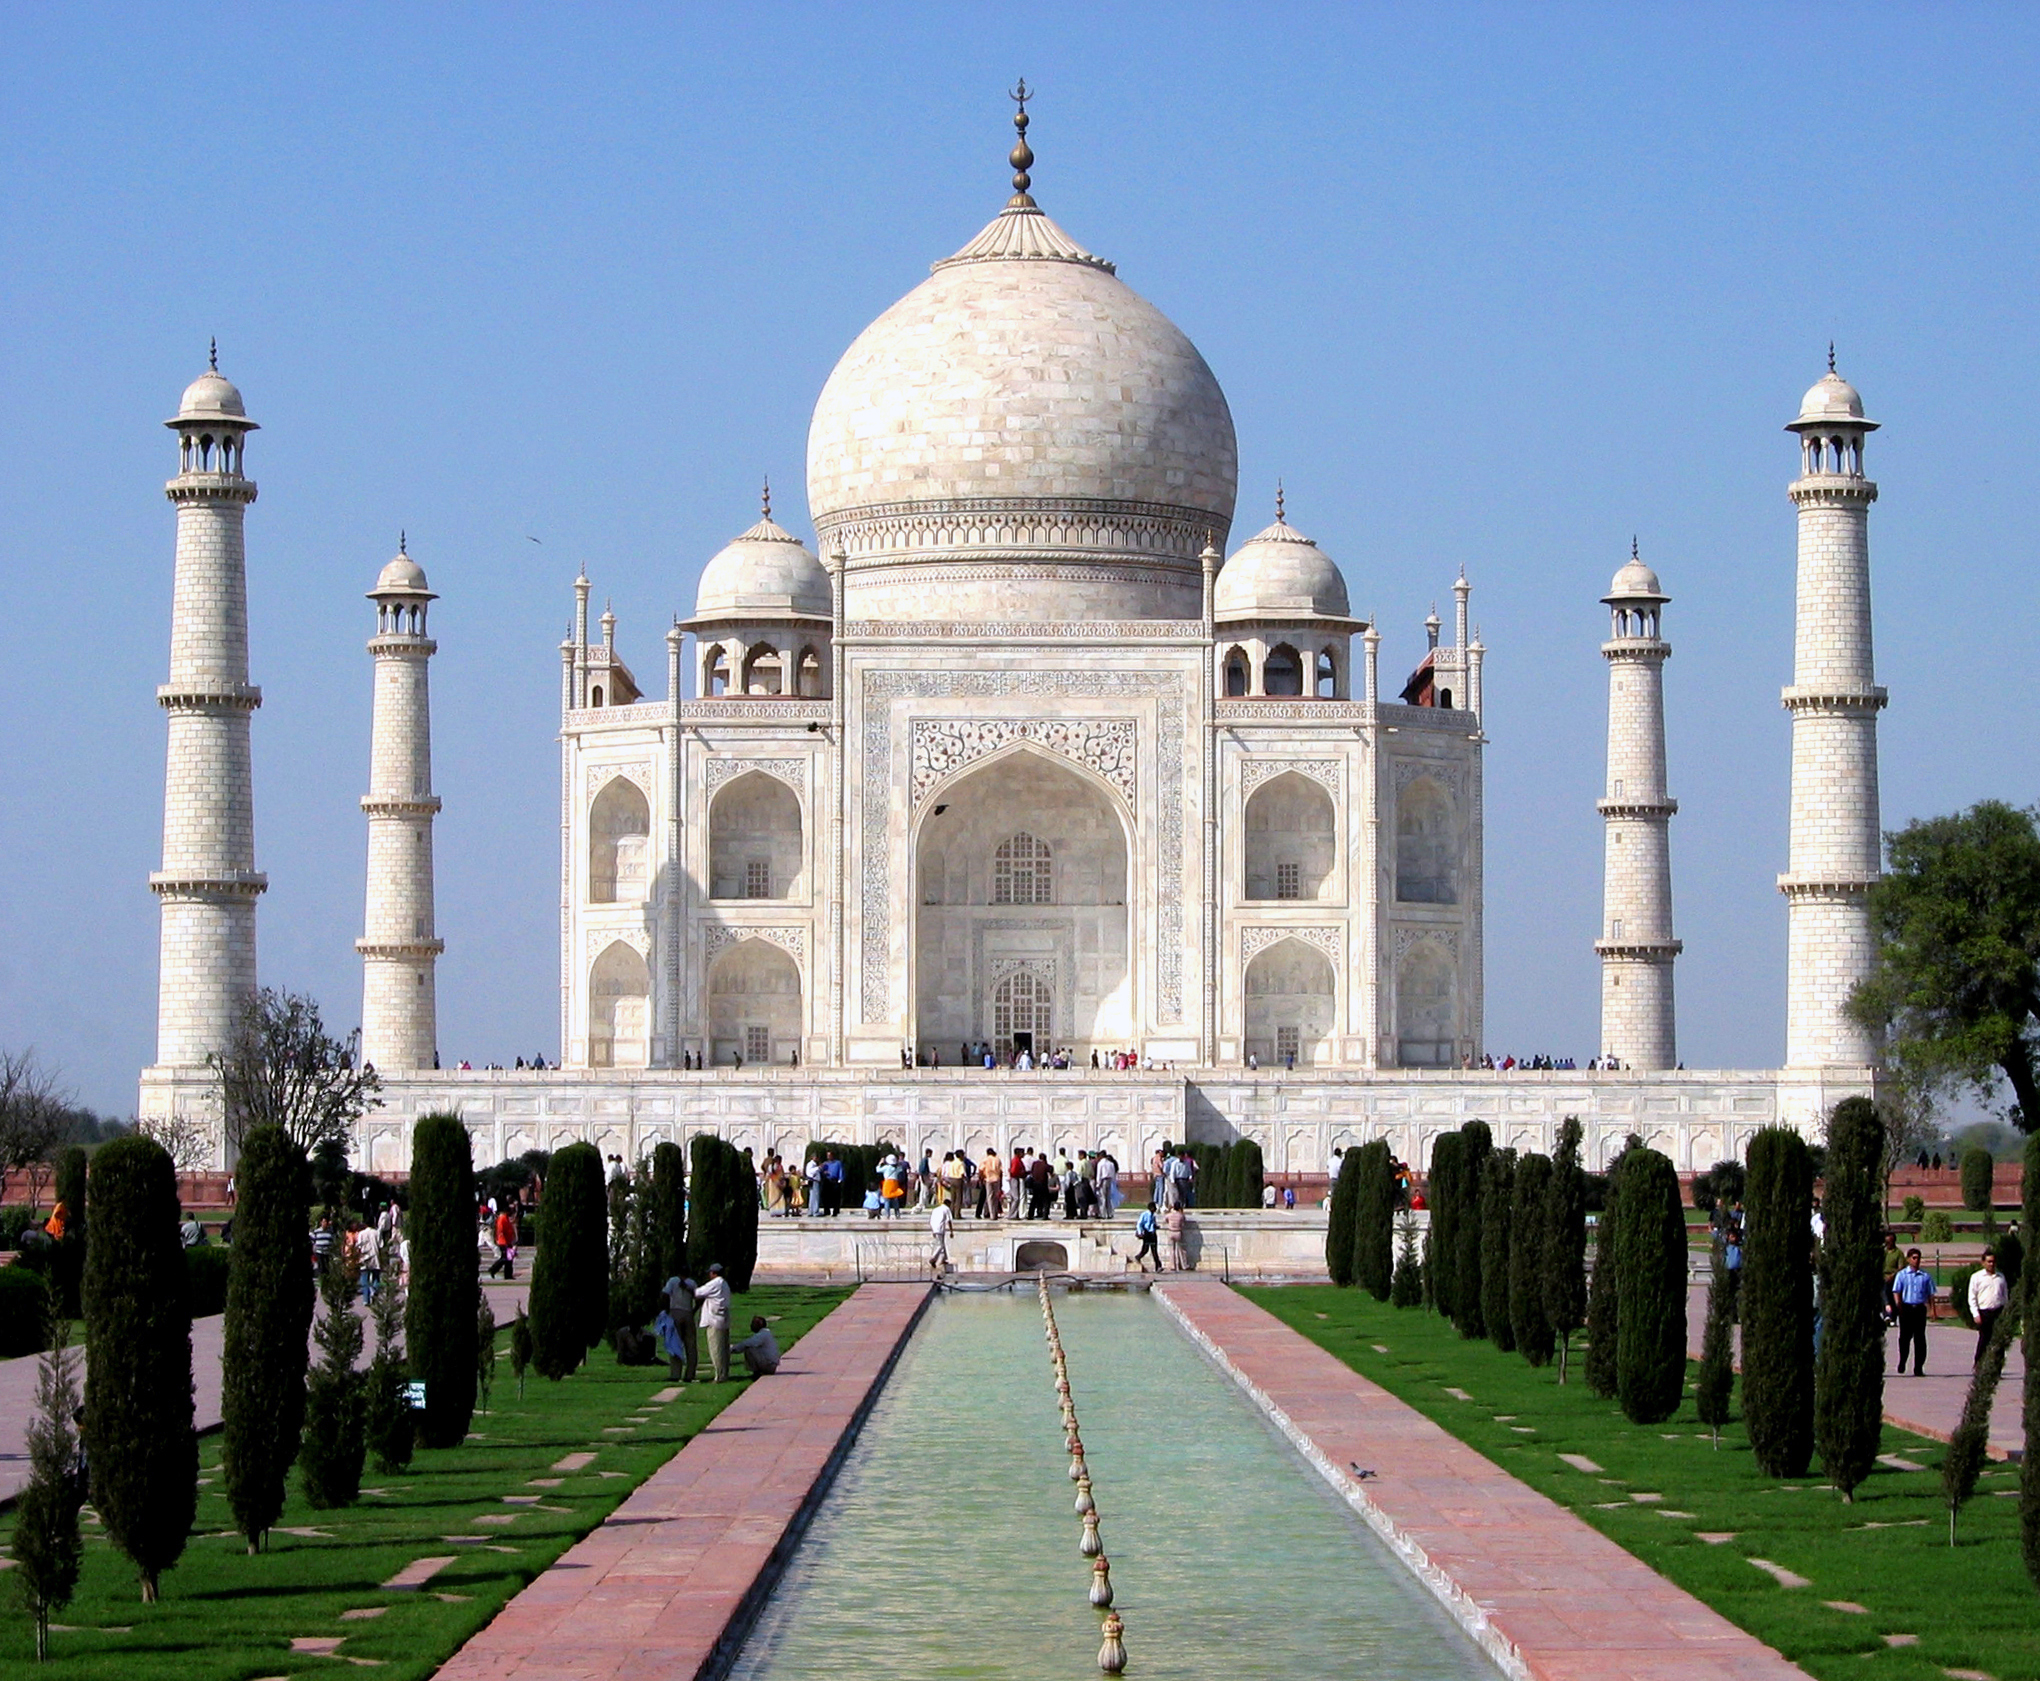
\includegraphics[width=20mm,scale=0.7]{images/taj_mahal.jpg}};}
	\onslide<2->{  \node [right=4.3cm of input_taj.south,anchor=south west] (raw)  { 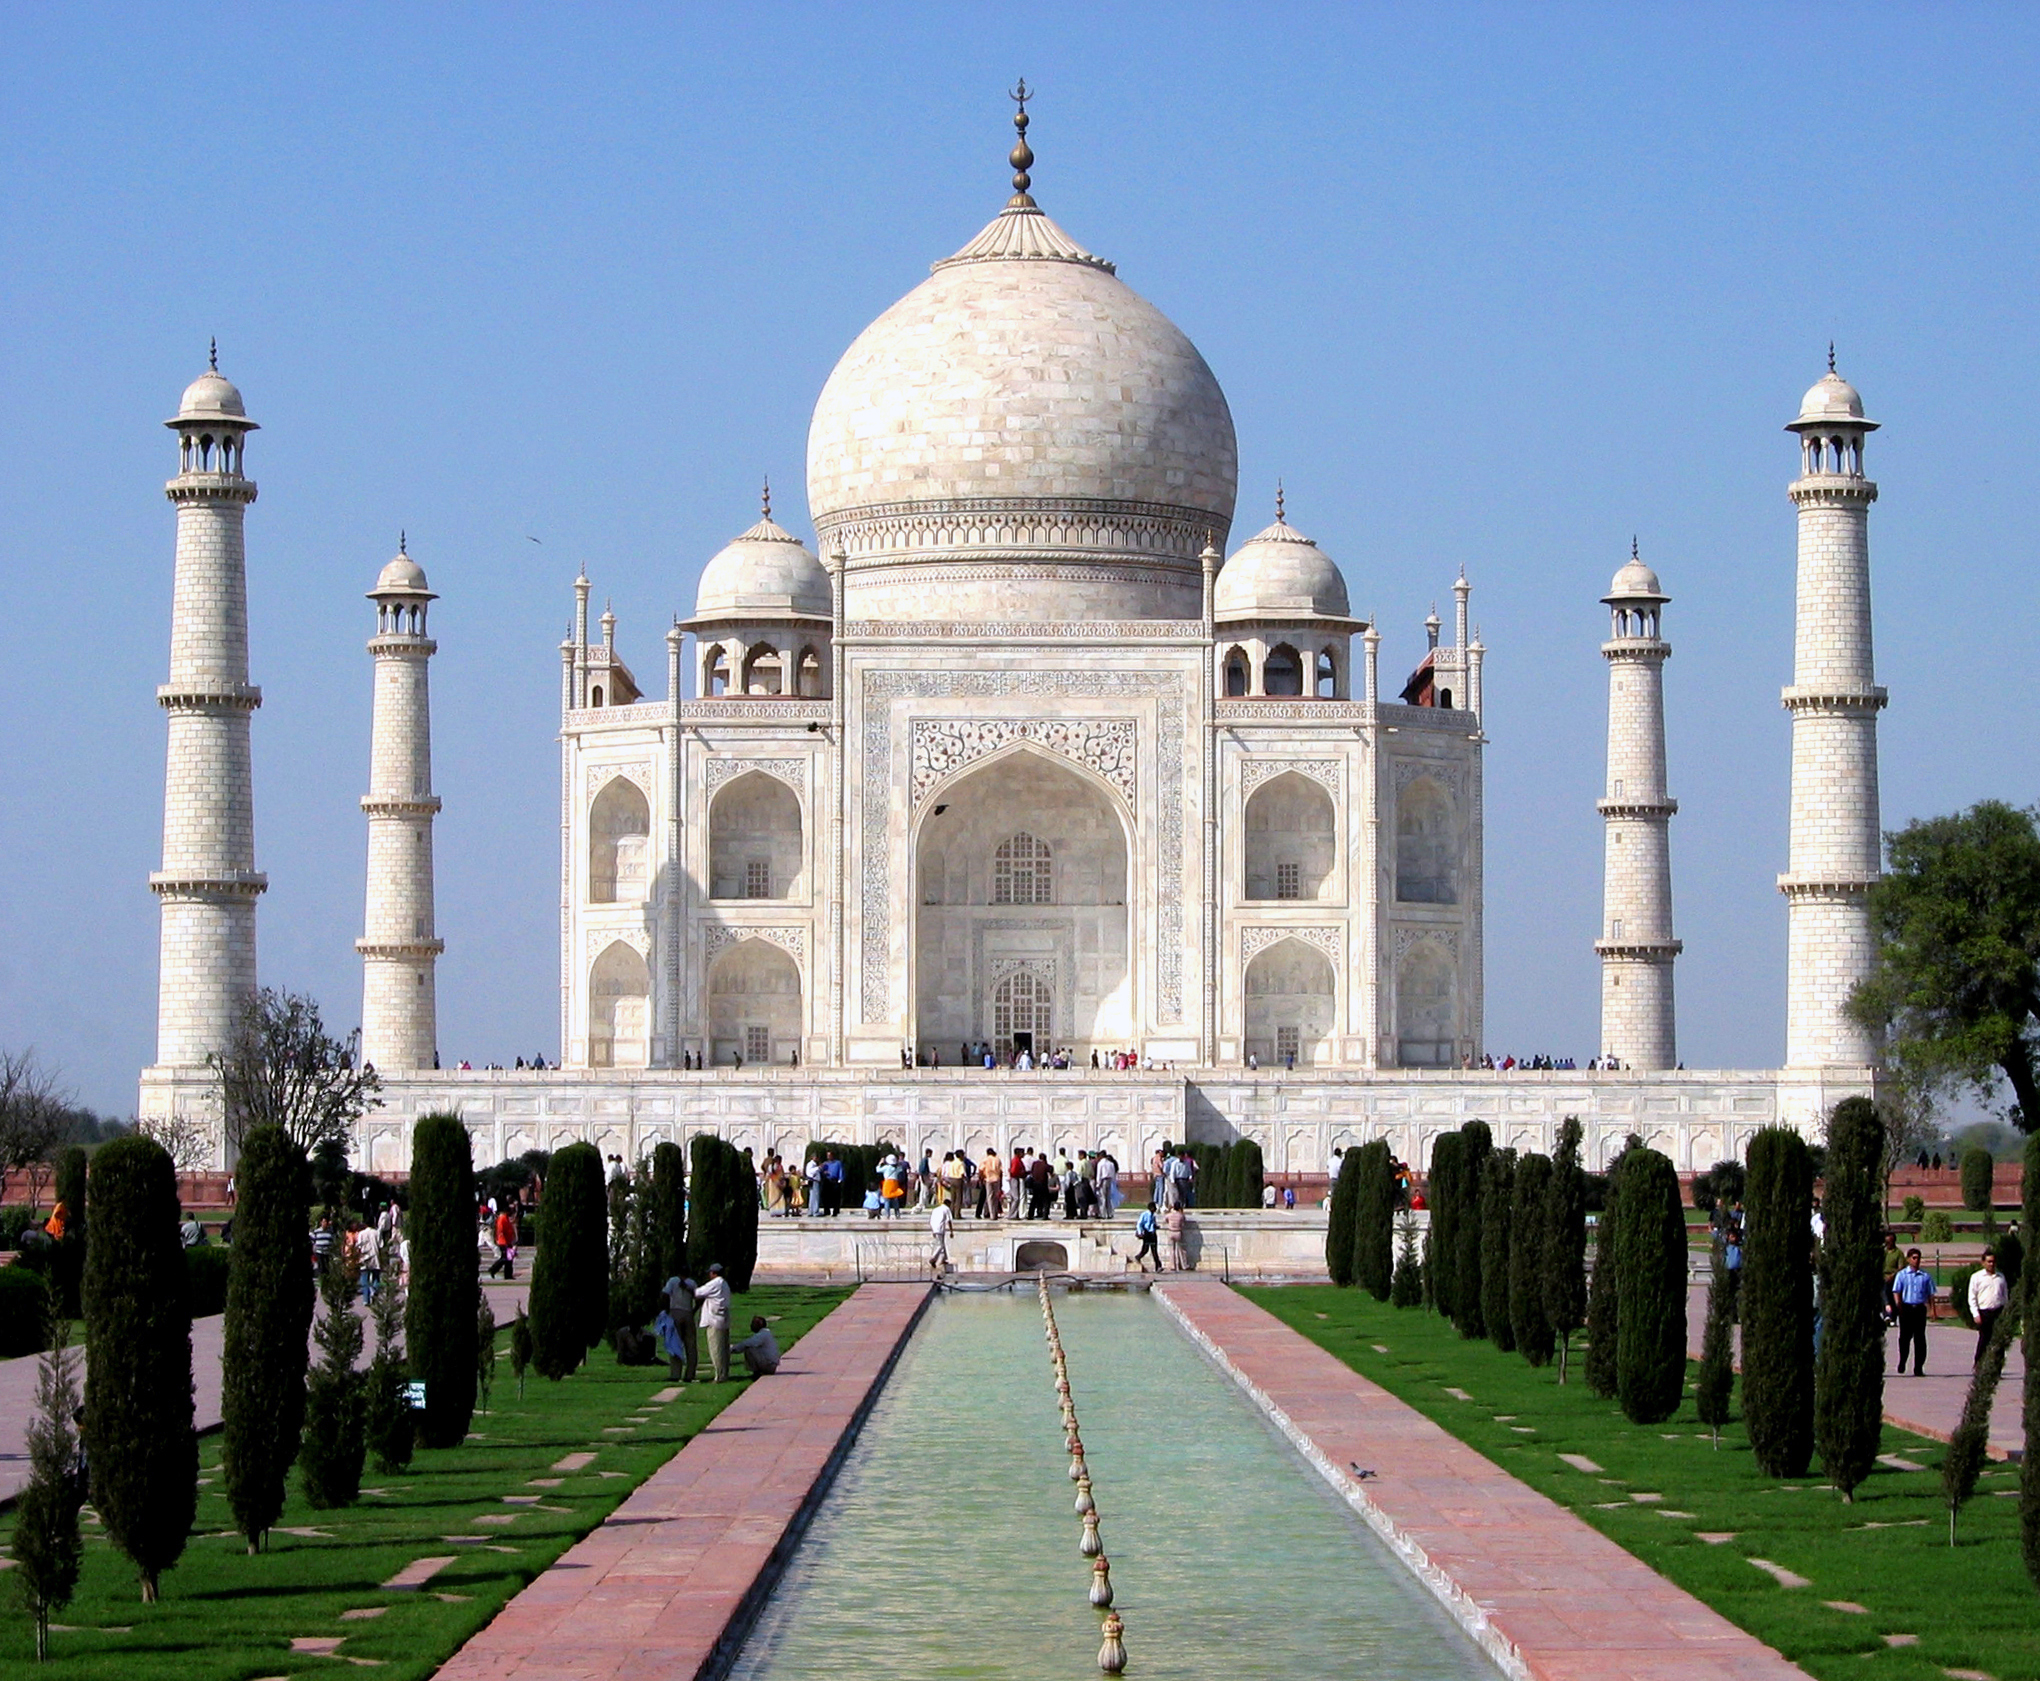
\includegraphics[width=20mm,scale=0.7]{images/taj_mahal.jpg}};

		\node[above of= raw,node distance=1.2cm ] (features)  {Features};
		\draw[->,thick] (input_taj) -- node [midway, above] {\footnotesize{$Raw\,pixels$}} (raw) ;}
	\onslide<3->{\node [right=5cm of raw.center,anchor= center](output_taj){car, bus, \textcolor{blue}{monument}, flower};
		\draw[->,thick] (raw) -- (output_taj) ;}
\end{tikzpicture}
	\end{minipage}
	
	\begin{minipage}[t]{0.25\textwidth}
		\begin{tikzpicture}
	\onslide<4->{ \node[] (input_taj) 
		{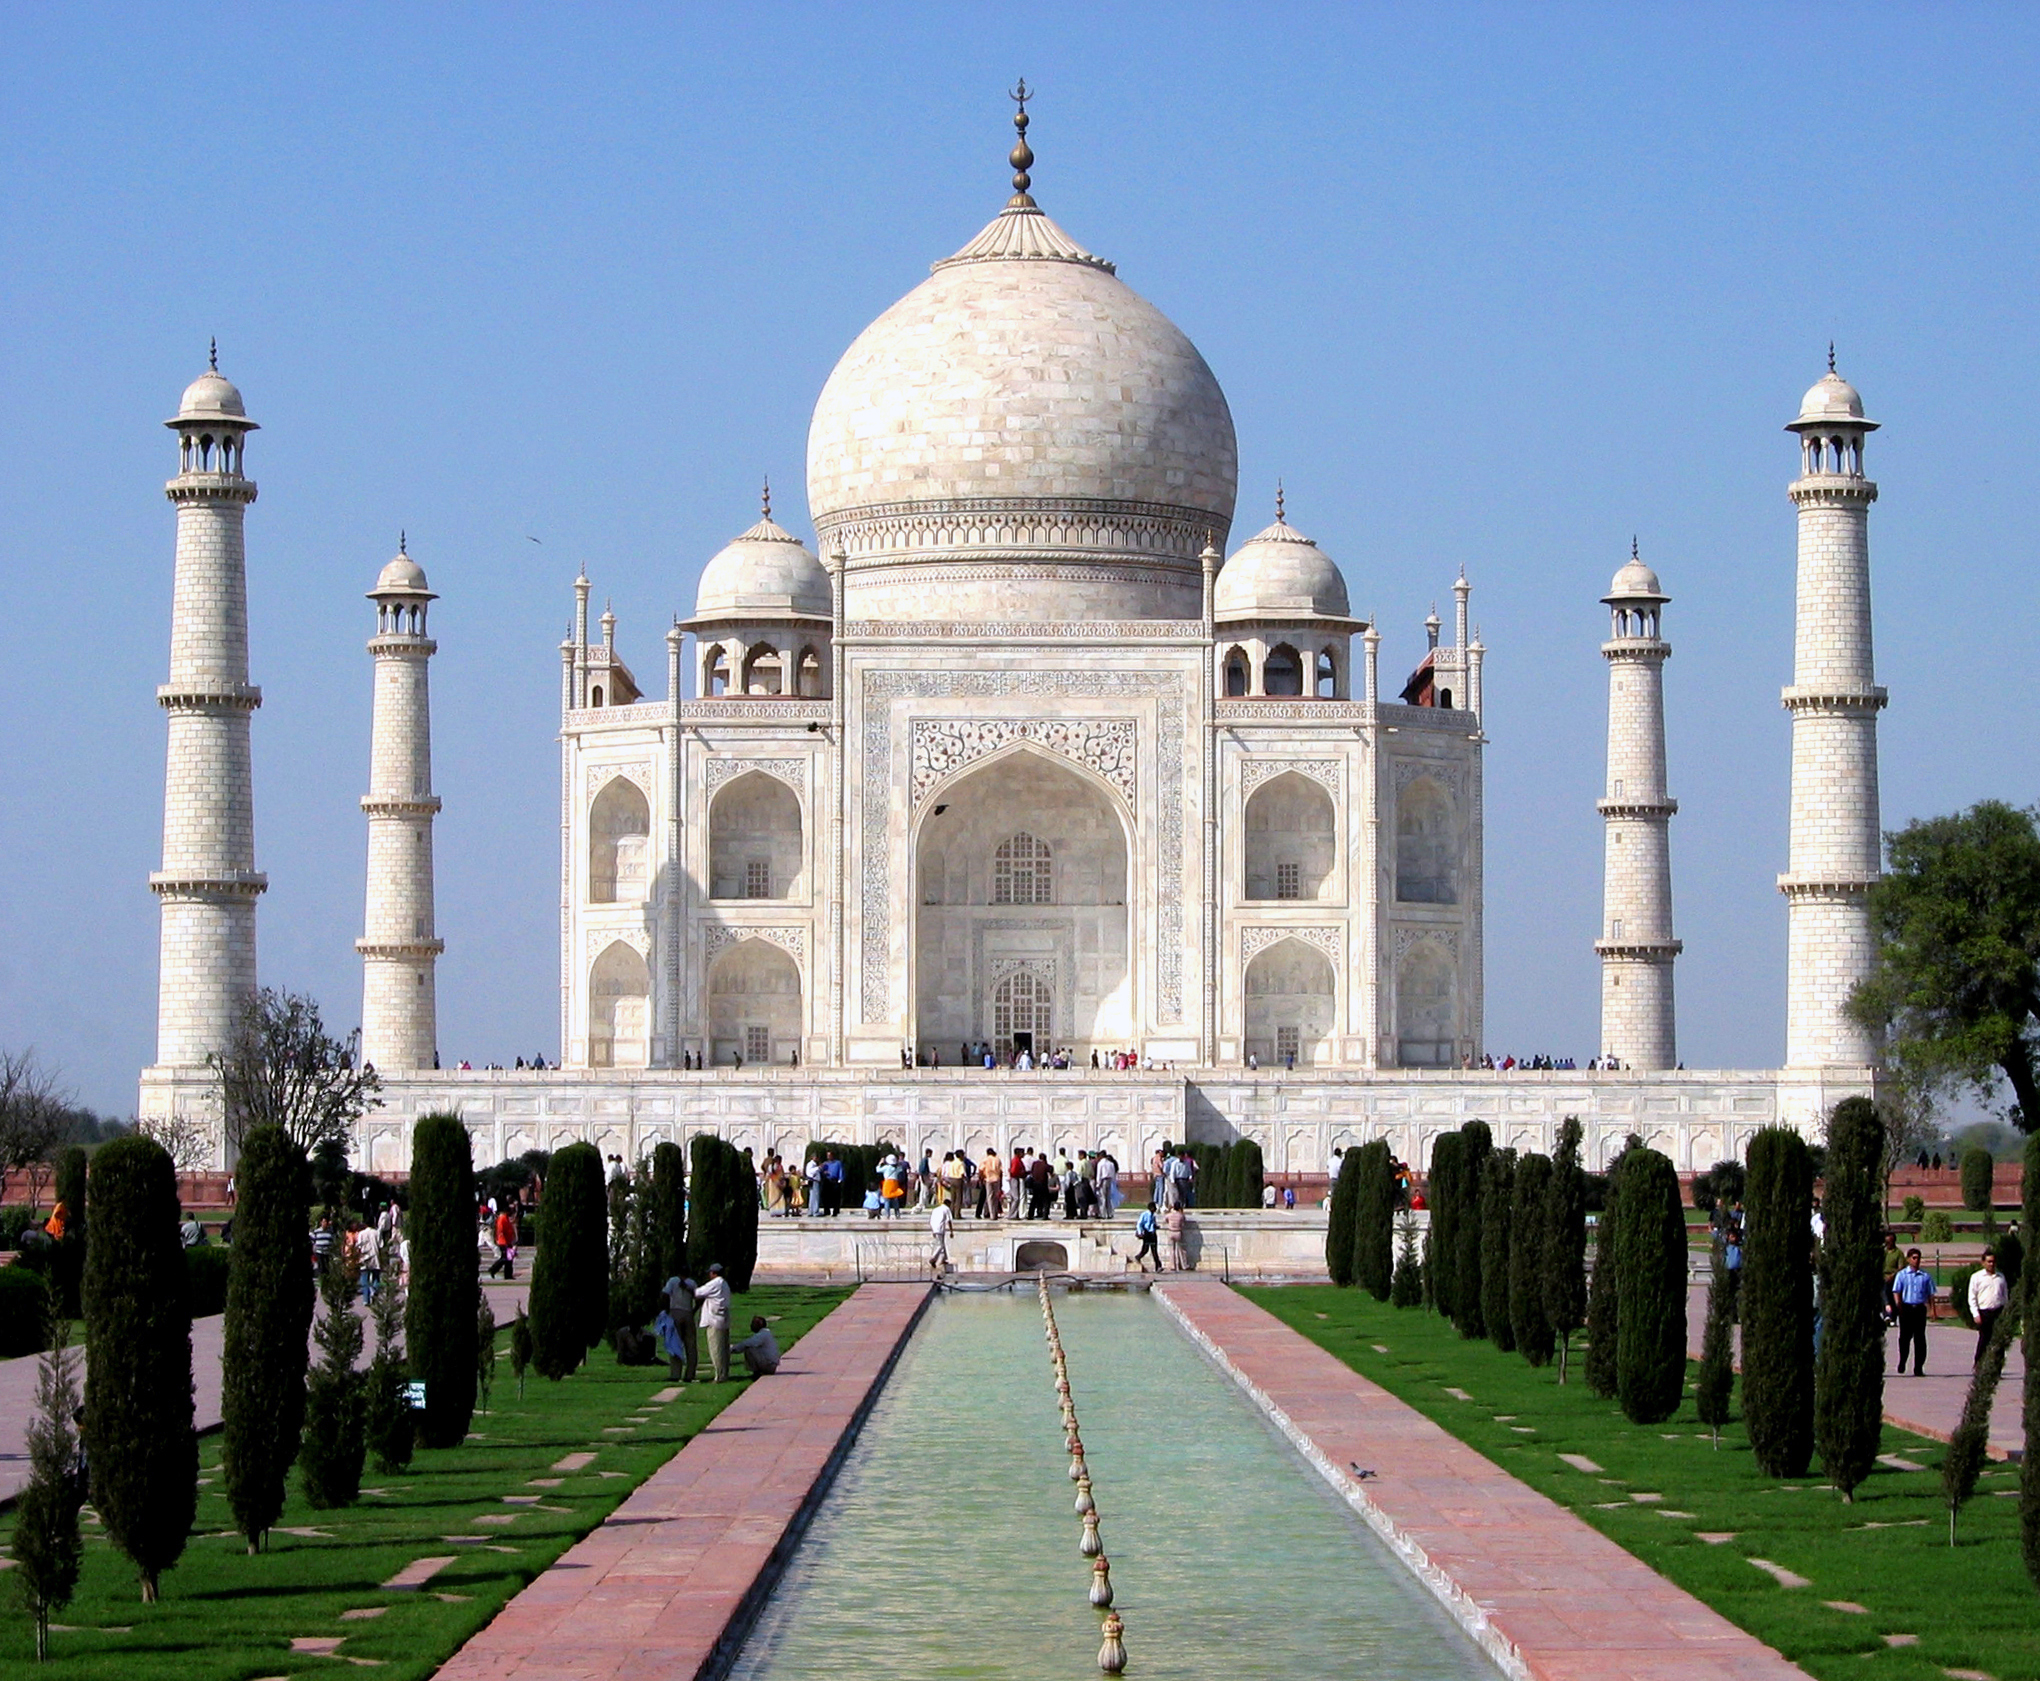
\includegraphics[width=20mm,scale=0.7]{images/taj_mahal.jpg}};}
	\onslide<5->{  \node [right=4.3cm of input_taj.south,anchor=south west] (edge)  { 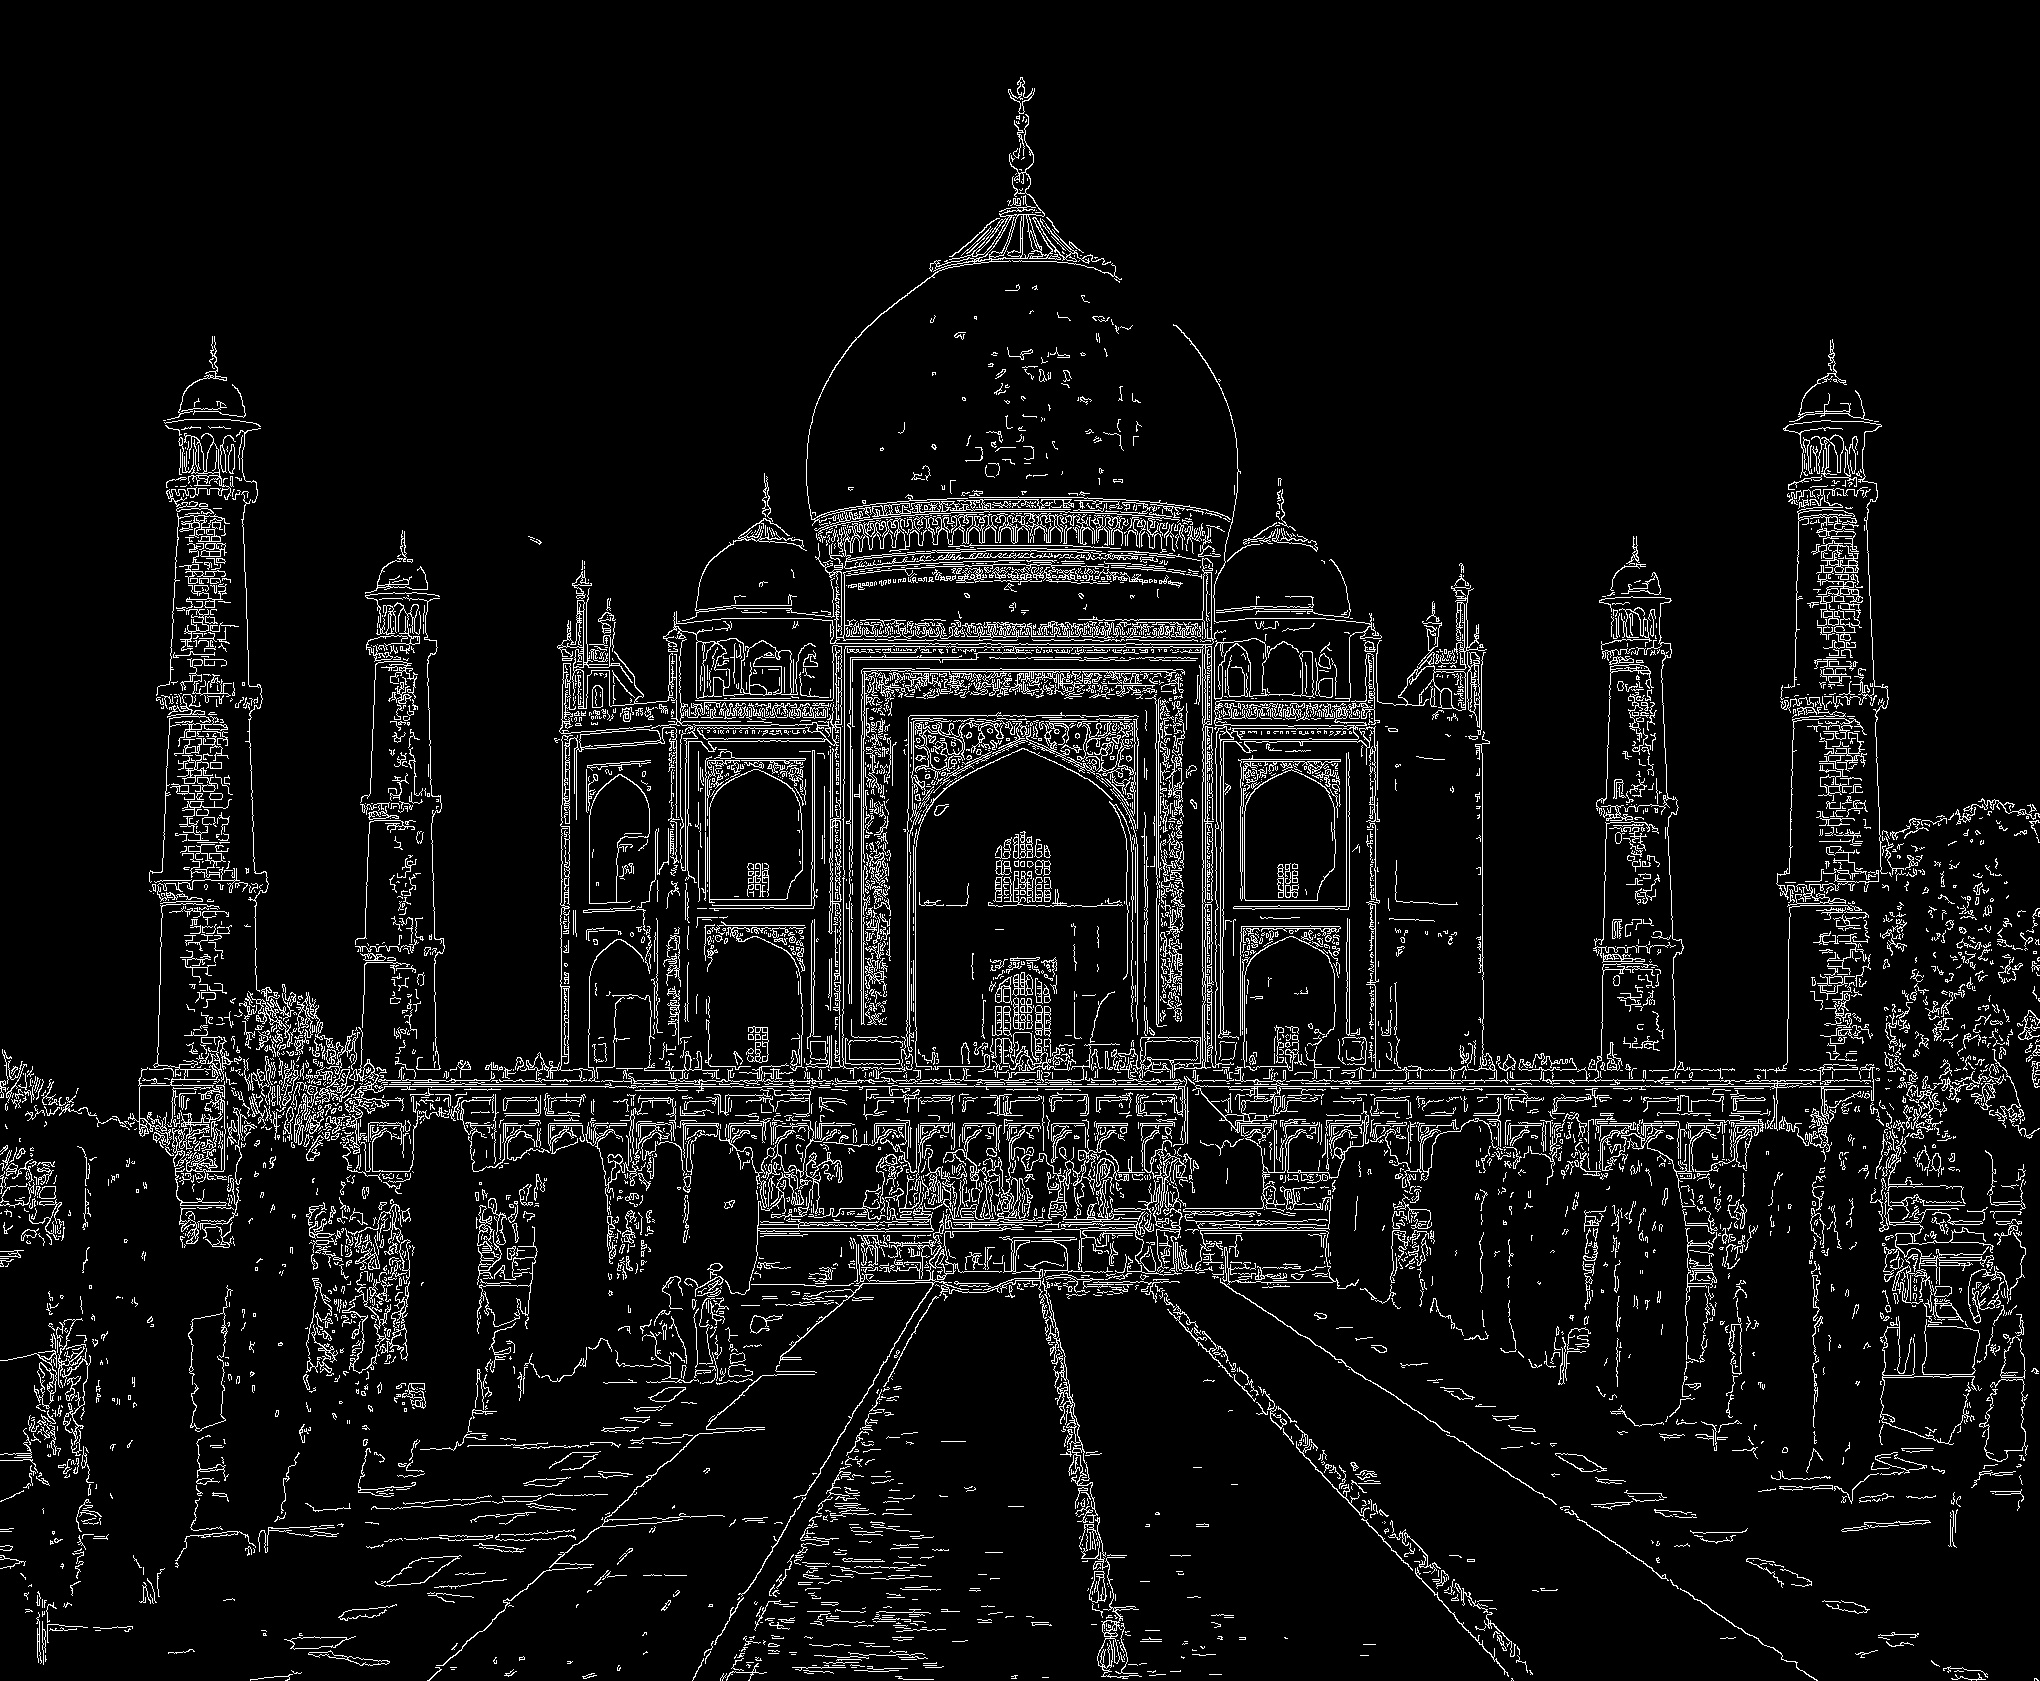
\includegraphics[width=20mm,scale=0.7]{images/taj_mahal_detectedges.jpg}};

		%\node[above of= raw,node distance=1.2cm ] (features)  {Features};
		\draw[->,thick] (input_taj) -- node [midway, above] {\footnotesize{$Edge\,Detector$}} (edge) ;}
	\onslide<6->{\node [right=5cm of edge.center,anchor= center](output_taj){car, bus, \textcolor{blue}{monument}, flower};
		\draw[->,thick] (edge) -- (output_taj) ;}

\end{tikzpicture}
	\end{minipage}
	
	\begin{minipage}[t]{0.25\textwidth}
		\begin{tikzpicture}
	\onslide<7->{ \node[] (input_taj) 
		{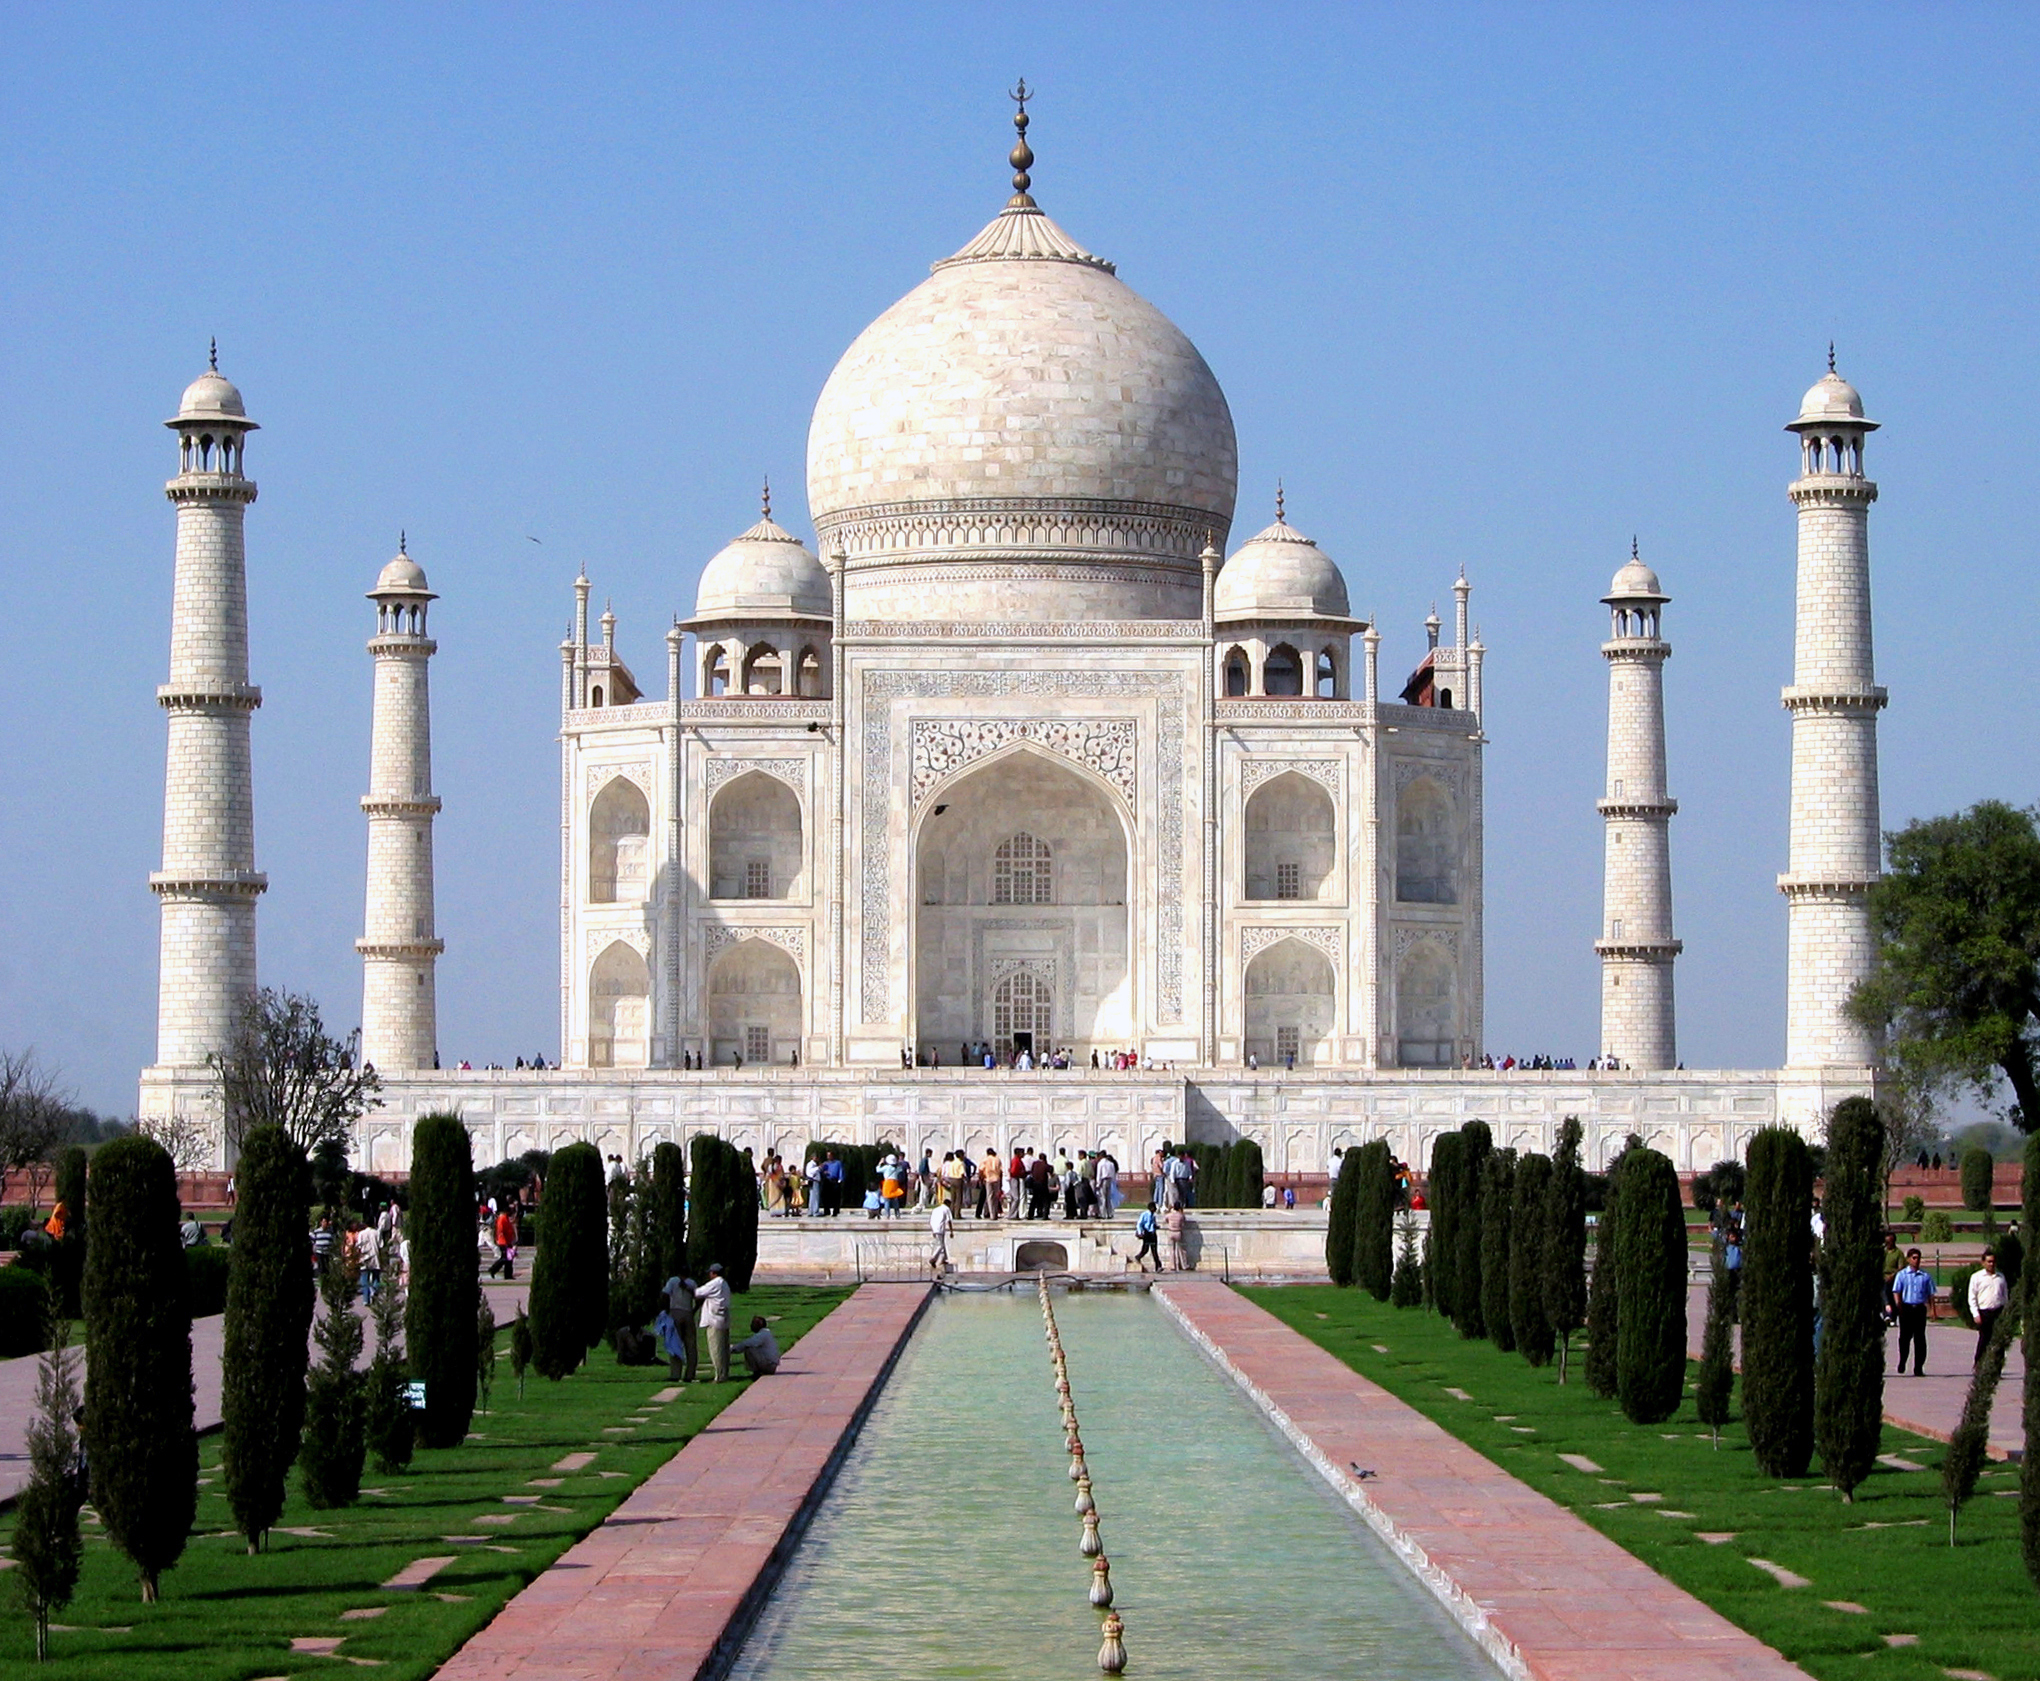
\includegraphics[width=20mm,scale=0.7]{images/taj_mahal.jpg}};}
	\onslide<8->{  \node [right=3cm of input_taj.south,anchor=south west] (sift)  {  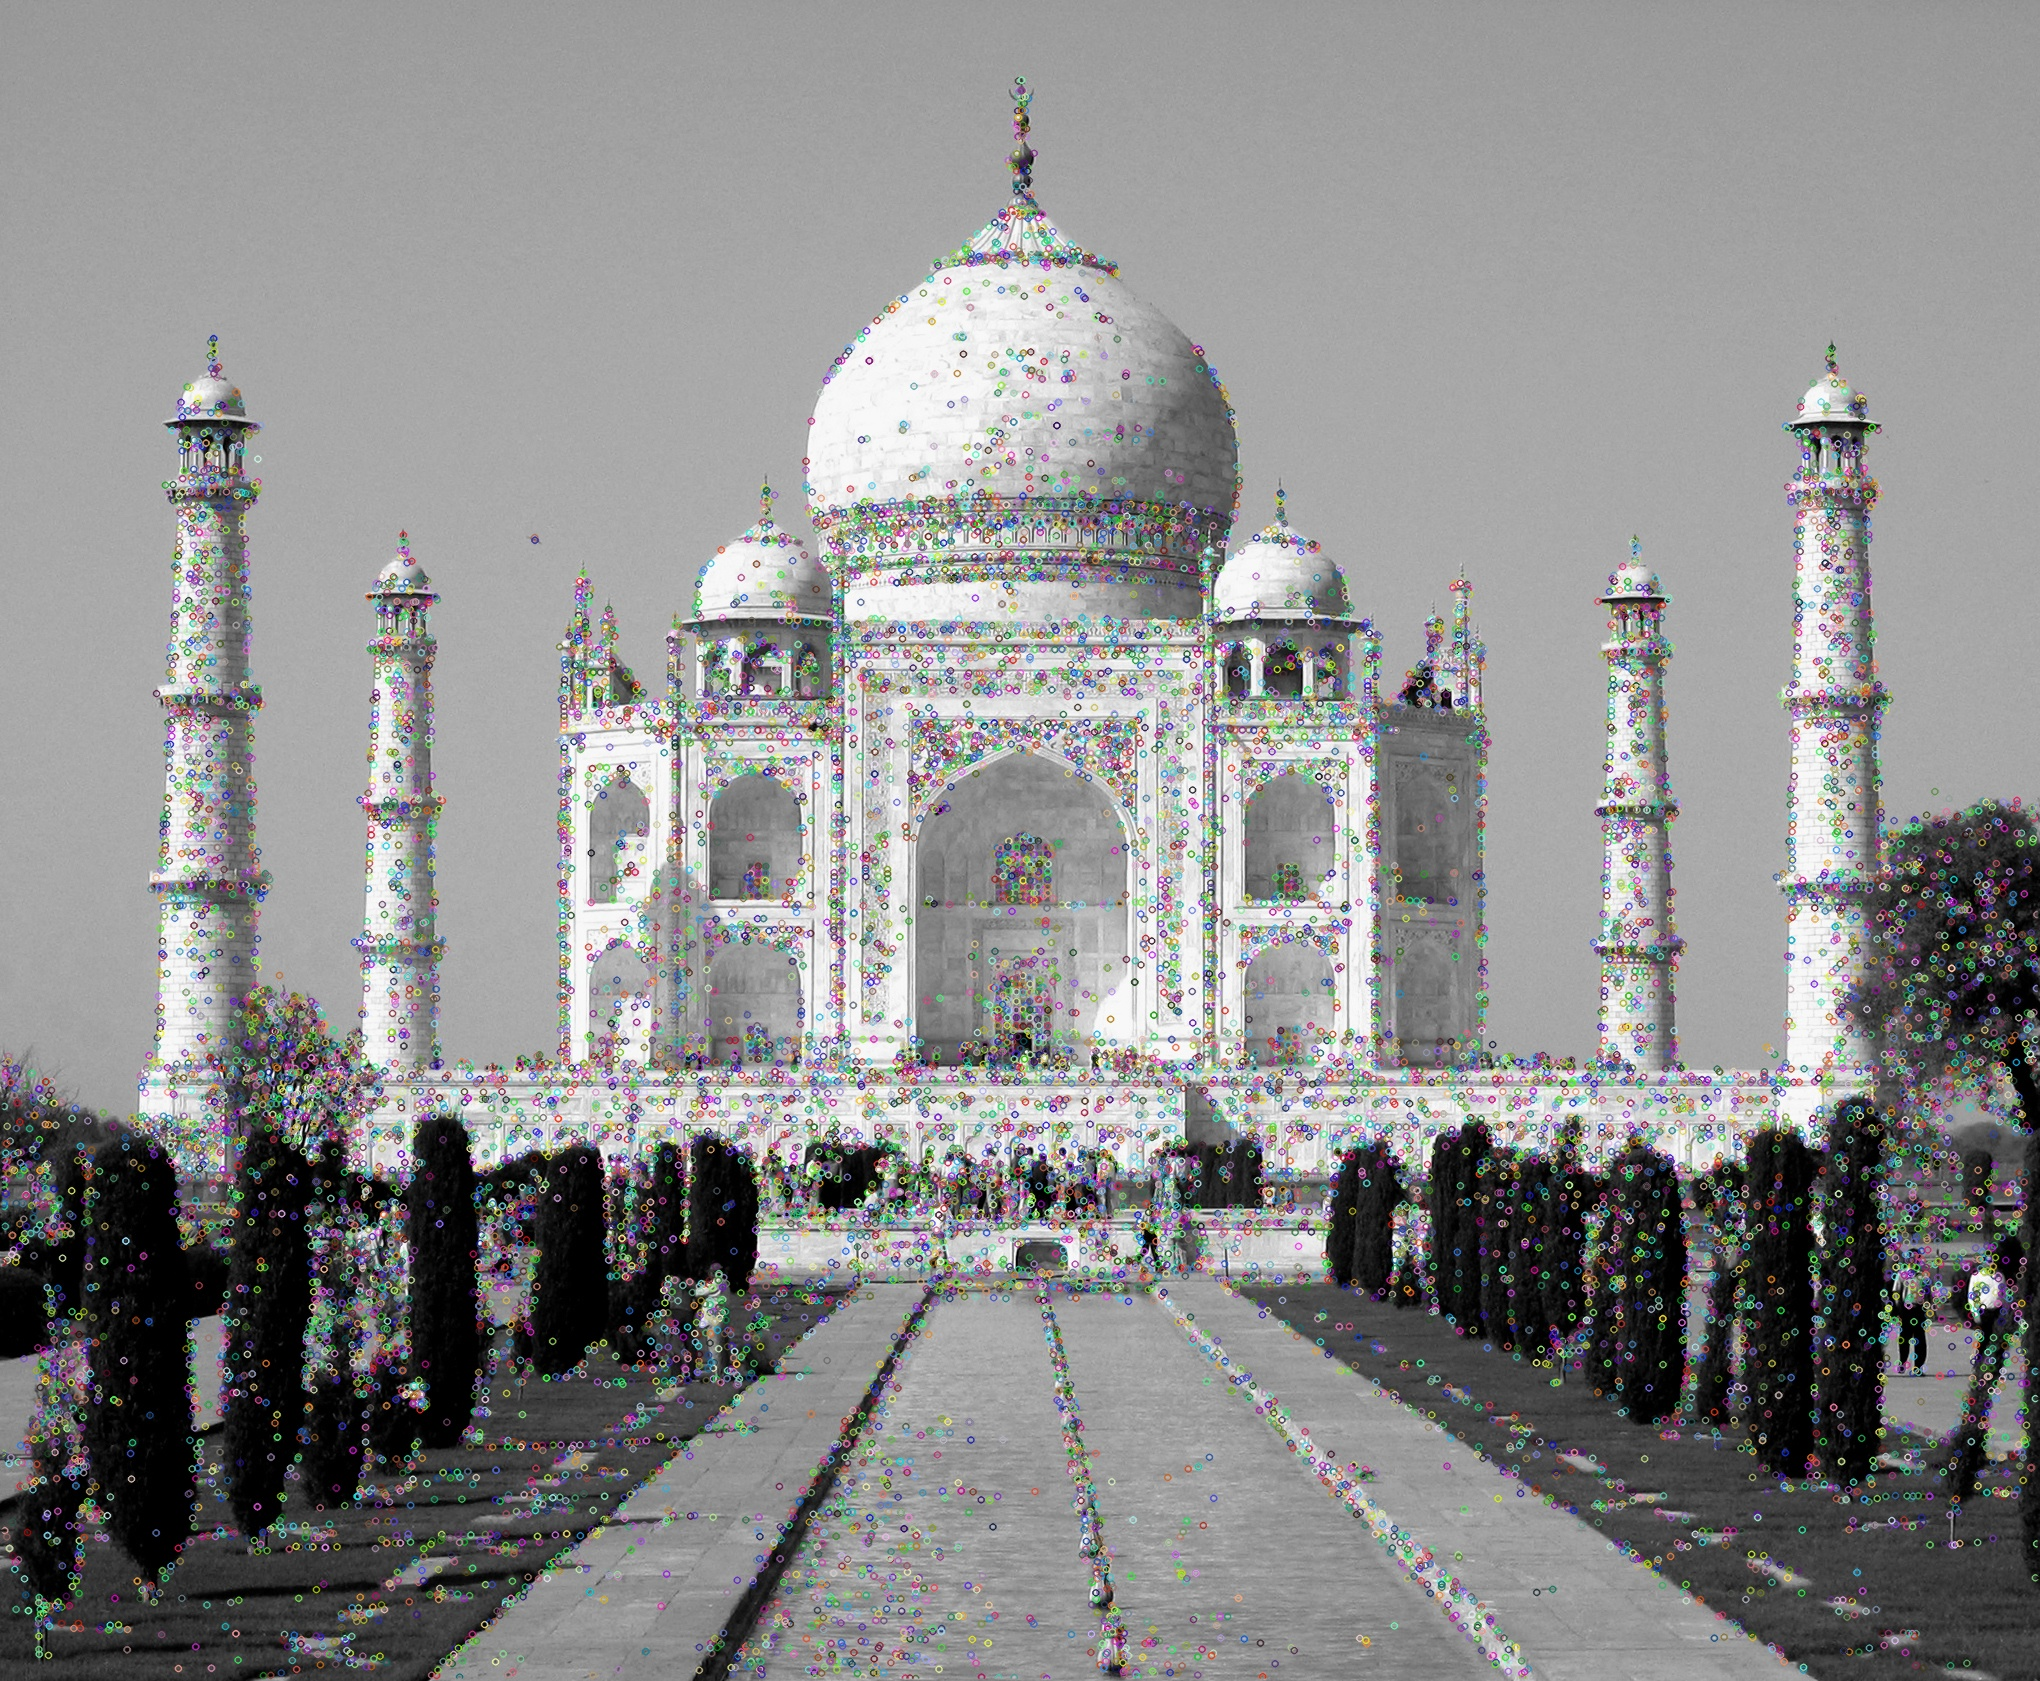
\includegraphics[width=20mm,scale=0.7]{images/SIFT.jpg}};
		\node [right= 0.1cm of sift] (hog)  { 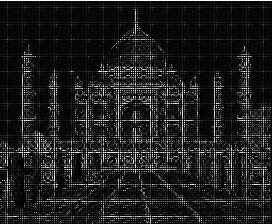
\includegraphics[width=20mm,scale=0.7]{images/hog.jpg}};
		%\node[above of= raw,node distance=1.2cm ] (features)  {Features};
		\draw[->,thick] (input_taj) -- node [name=u,midway, above] {\footnotesize{$SIFT/HOG$}} (sift) ;}
	% \onslide<8->{  \node [right= of hog] (sift)  { 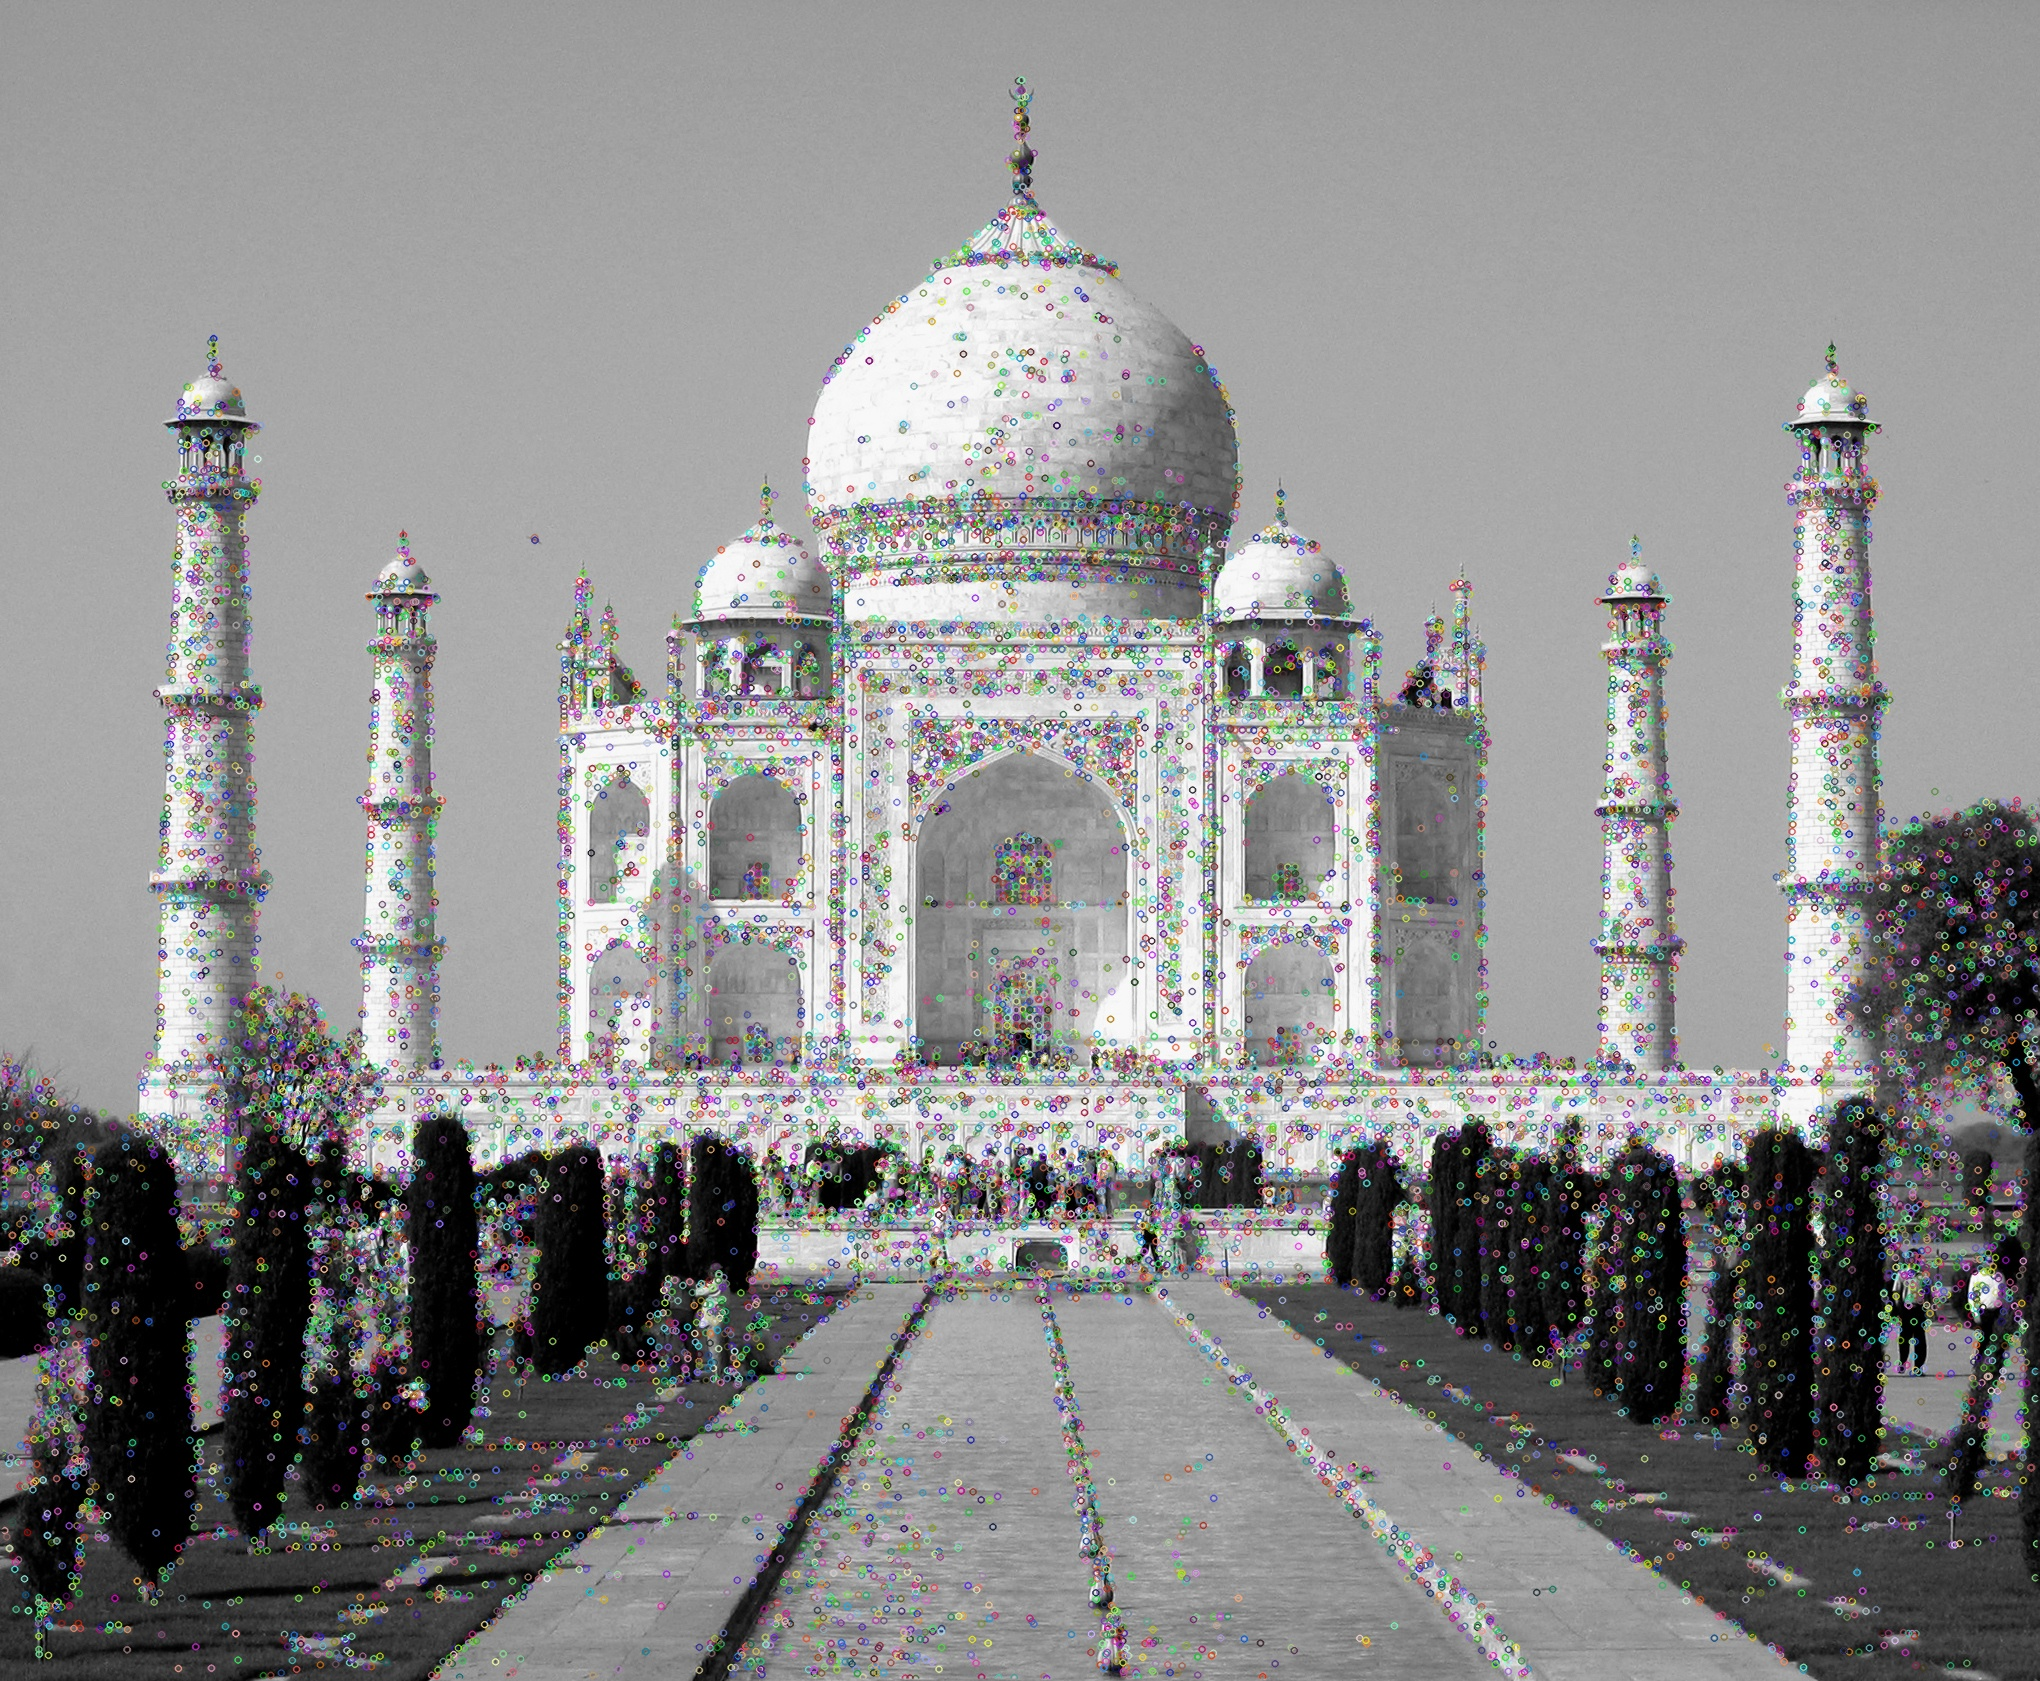
\includegraphics[width=20mm,scale=0.7]{SIFT1.jpg}};
	\onslide<9->{\node [right=4cm of hog.center,anchor= center](output_taj){car, bus, \textcolor{blue}{monument}, flower};
		\draw[->,thick] (hog) -- node [name=v,midway, above]{$ $} (output_taj) ;}

	\onslide<10->{\draw [
			thick,
			decoration={
				brace,
				mirror,
				raise=0.9cm
			},
			decorate
		] (u.south east) -- (hog.east) 
		node [pos=0.5,anchor=north,yshift=-0.9cm,font=\footnotesize] {static feature extraction (no learning)}; 
		\draw [
			thick,
			decoration={
				brace,
				mirror,
				raise=0.9cm
			},
			decorate
		] (v.south east) -- (output_taj.east) 
		node [pos=0.5,anchor=north,yshift=-0.9cm,font=\footnotesize] {learning weights of classifier};
	}
\end{tikzpicture}
	\end{minipage}
	
\end{frame}


%%%%%%%%%%%%%%%%%%%%%%%%%%%%%%%%%%%%%%%%%%%%%%%%%%%%%%%%%%%%%%%%%%%%%%%%%%%%%%%%%%%%%%%%%
\begin{frame}
	\begin{overlayarea}{\textwidth}{\textheight}
		\begin{minipage}[t]{0.25\textwidth}
			\begin{tikzpicture}[scale=0.9,transform shape] 
	\onslide<1->{ \node[] (input_taj) 
		{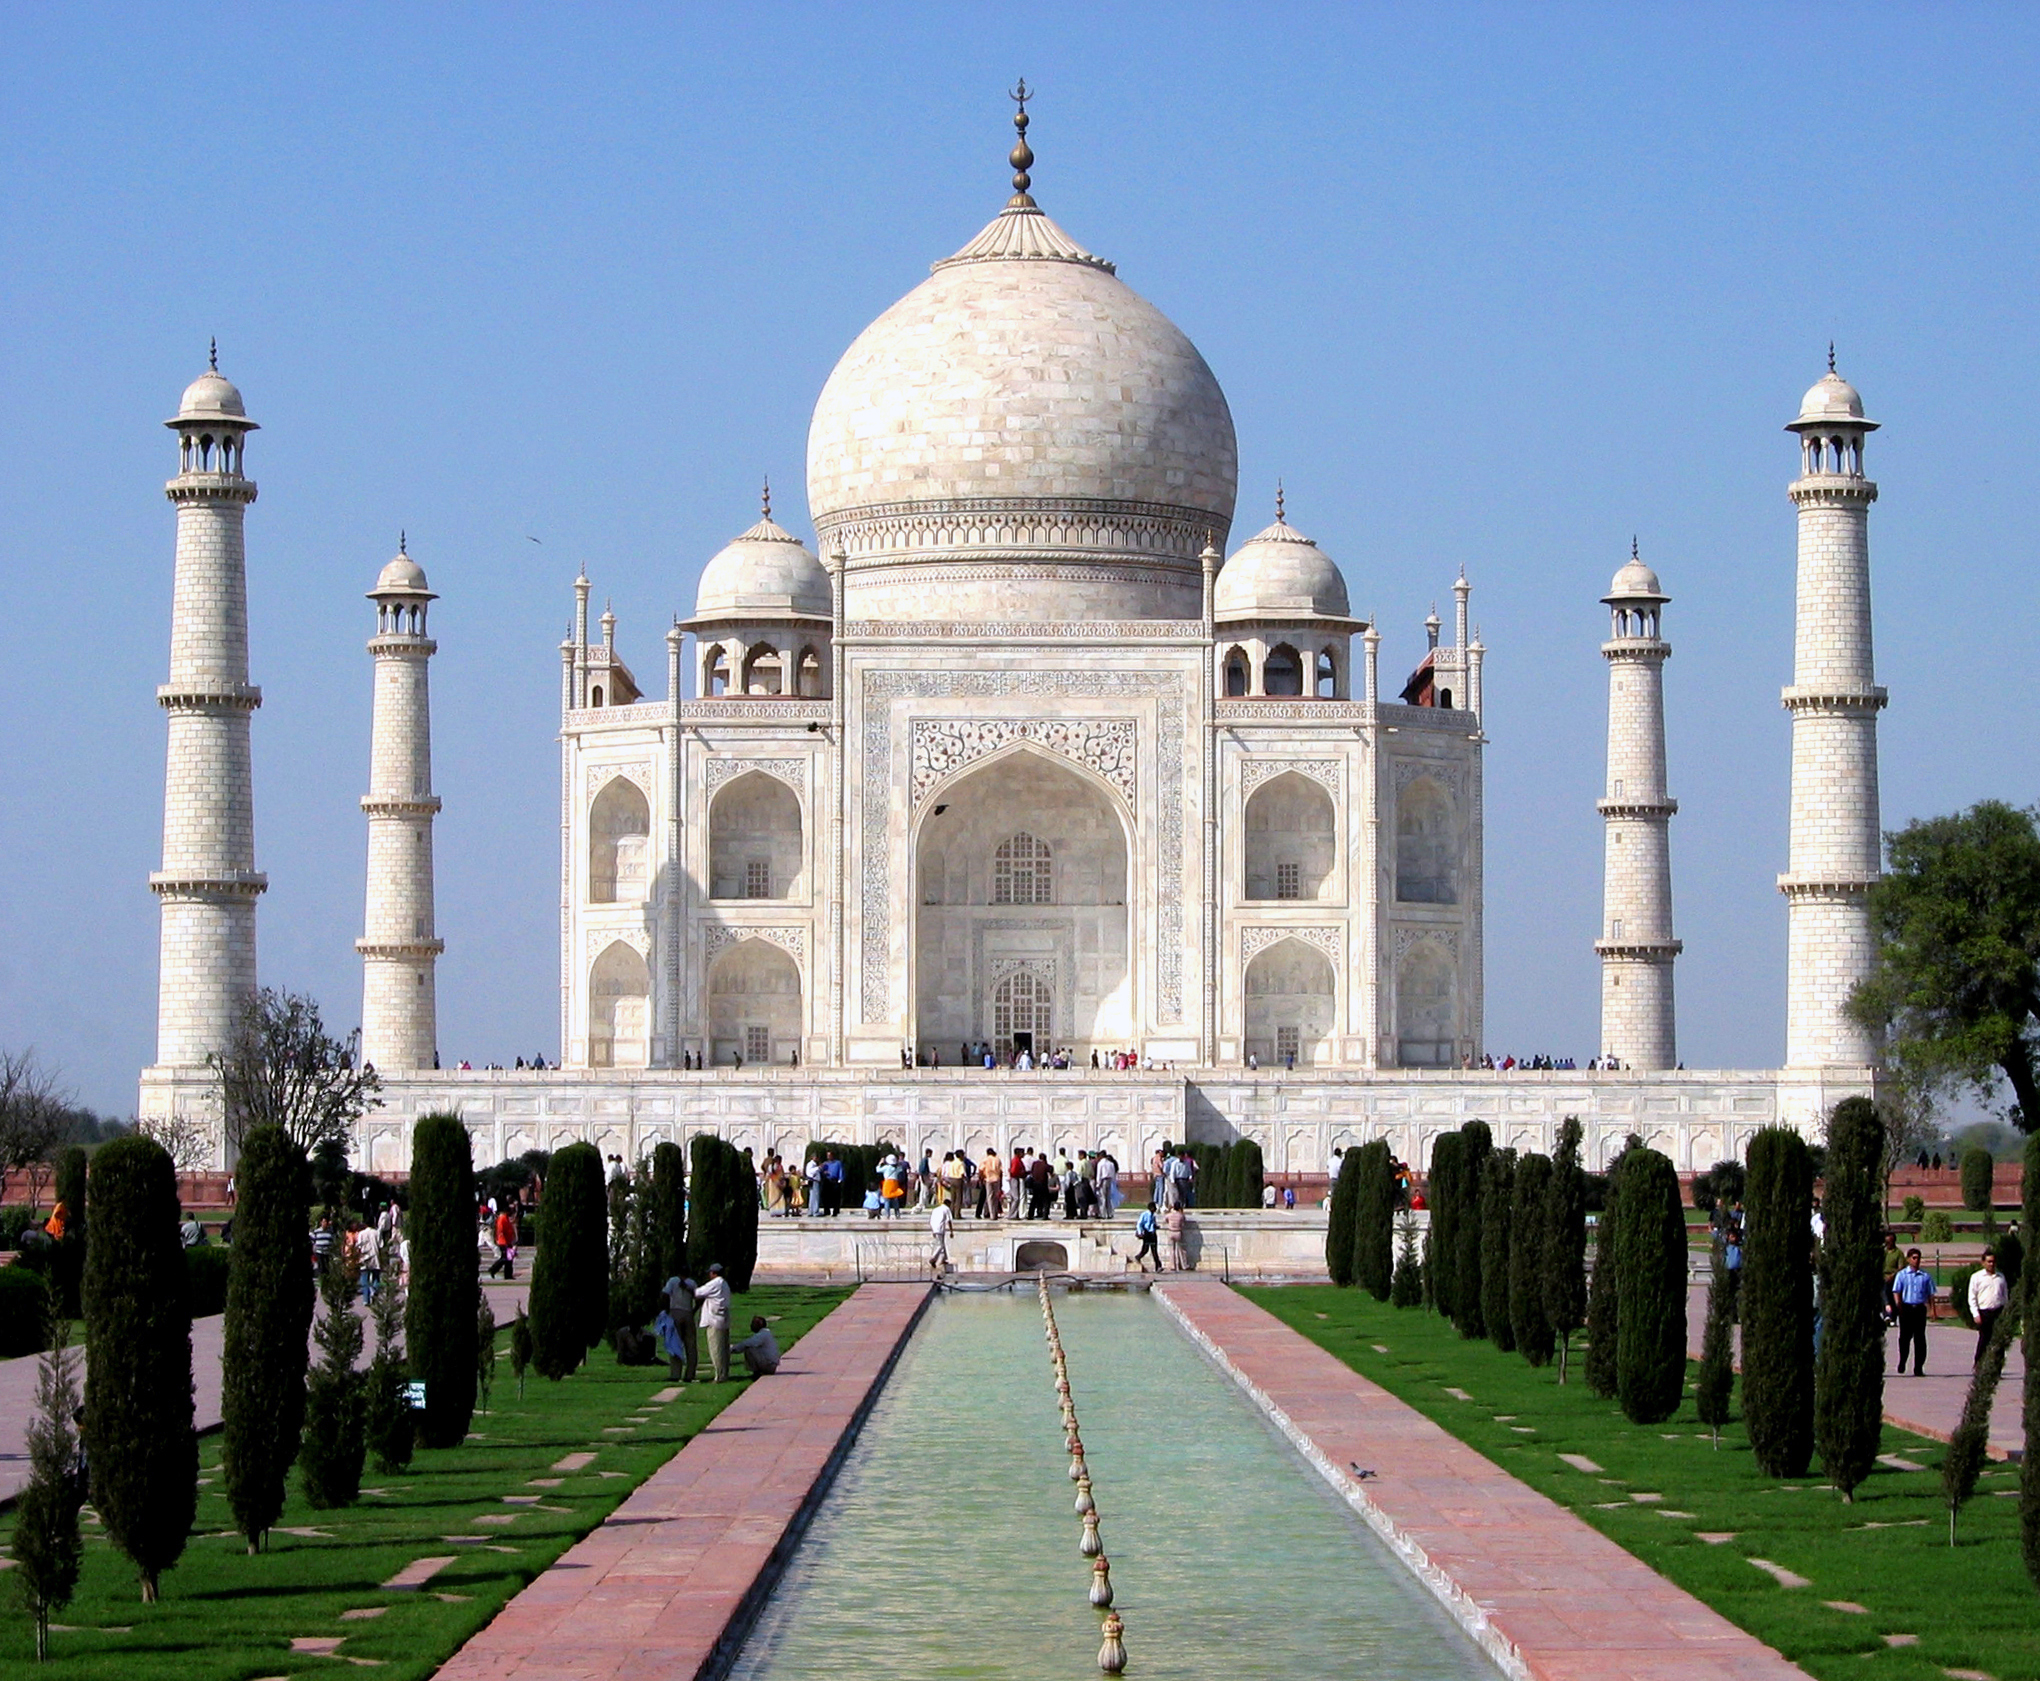
\includegraphics[width=20mm,scale=0.7]{images/taj_mahal.jpg}};
	}
	\onslide<1->{  \node [right=3cm of input_taj.south,anchor=south west] (raw)  { 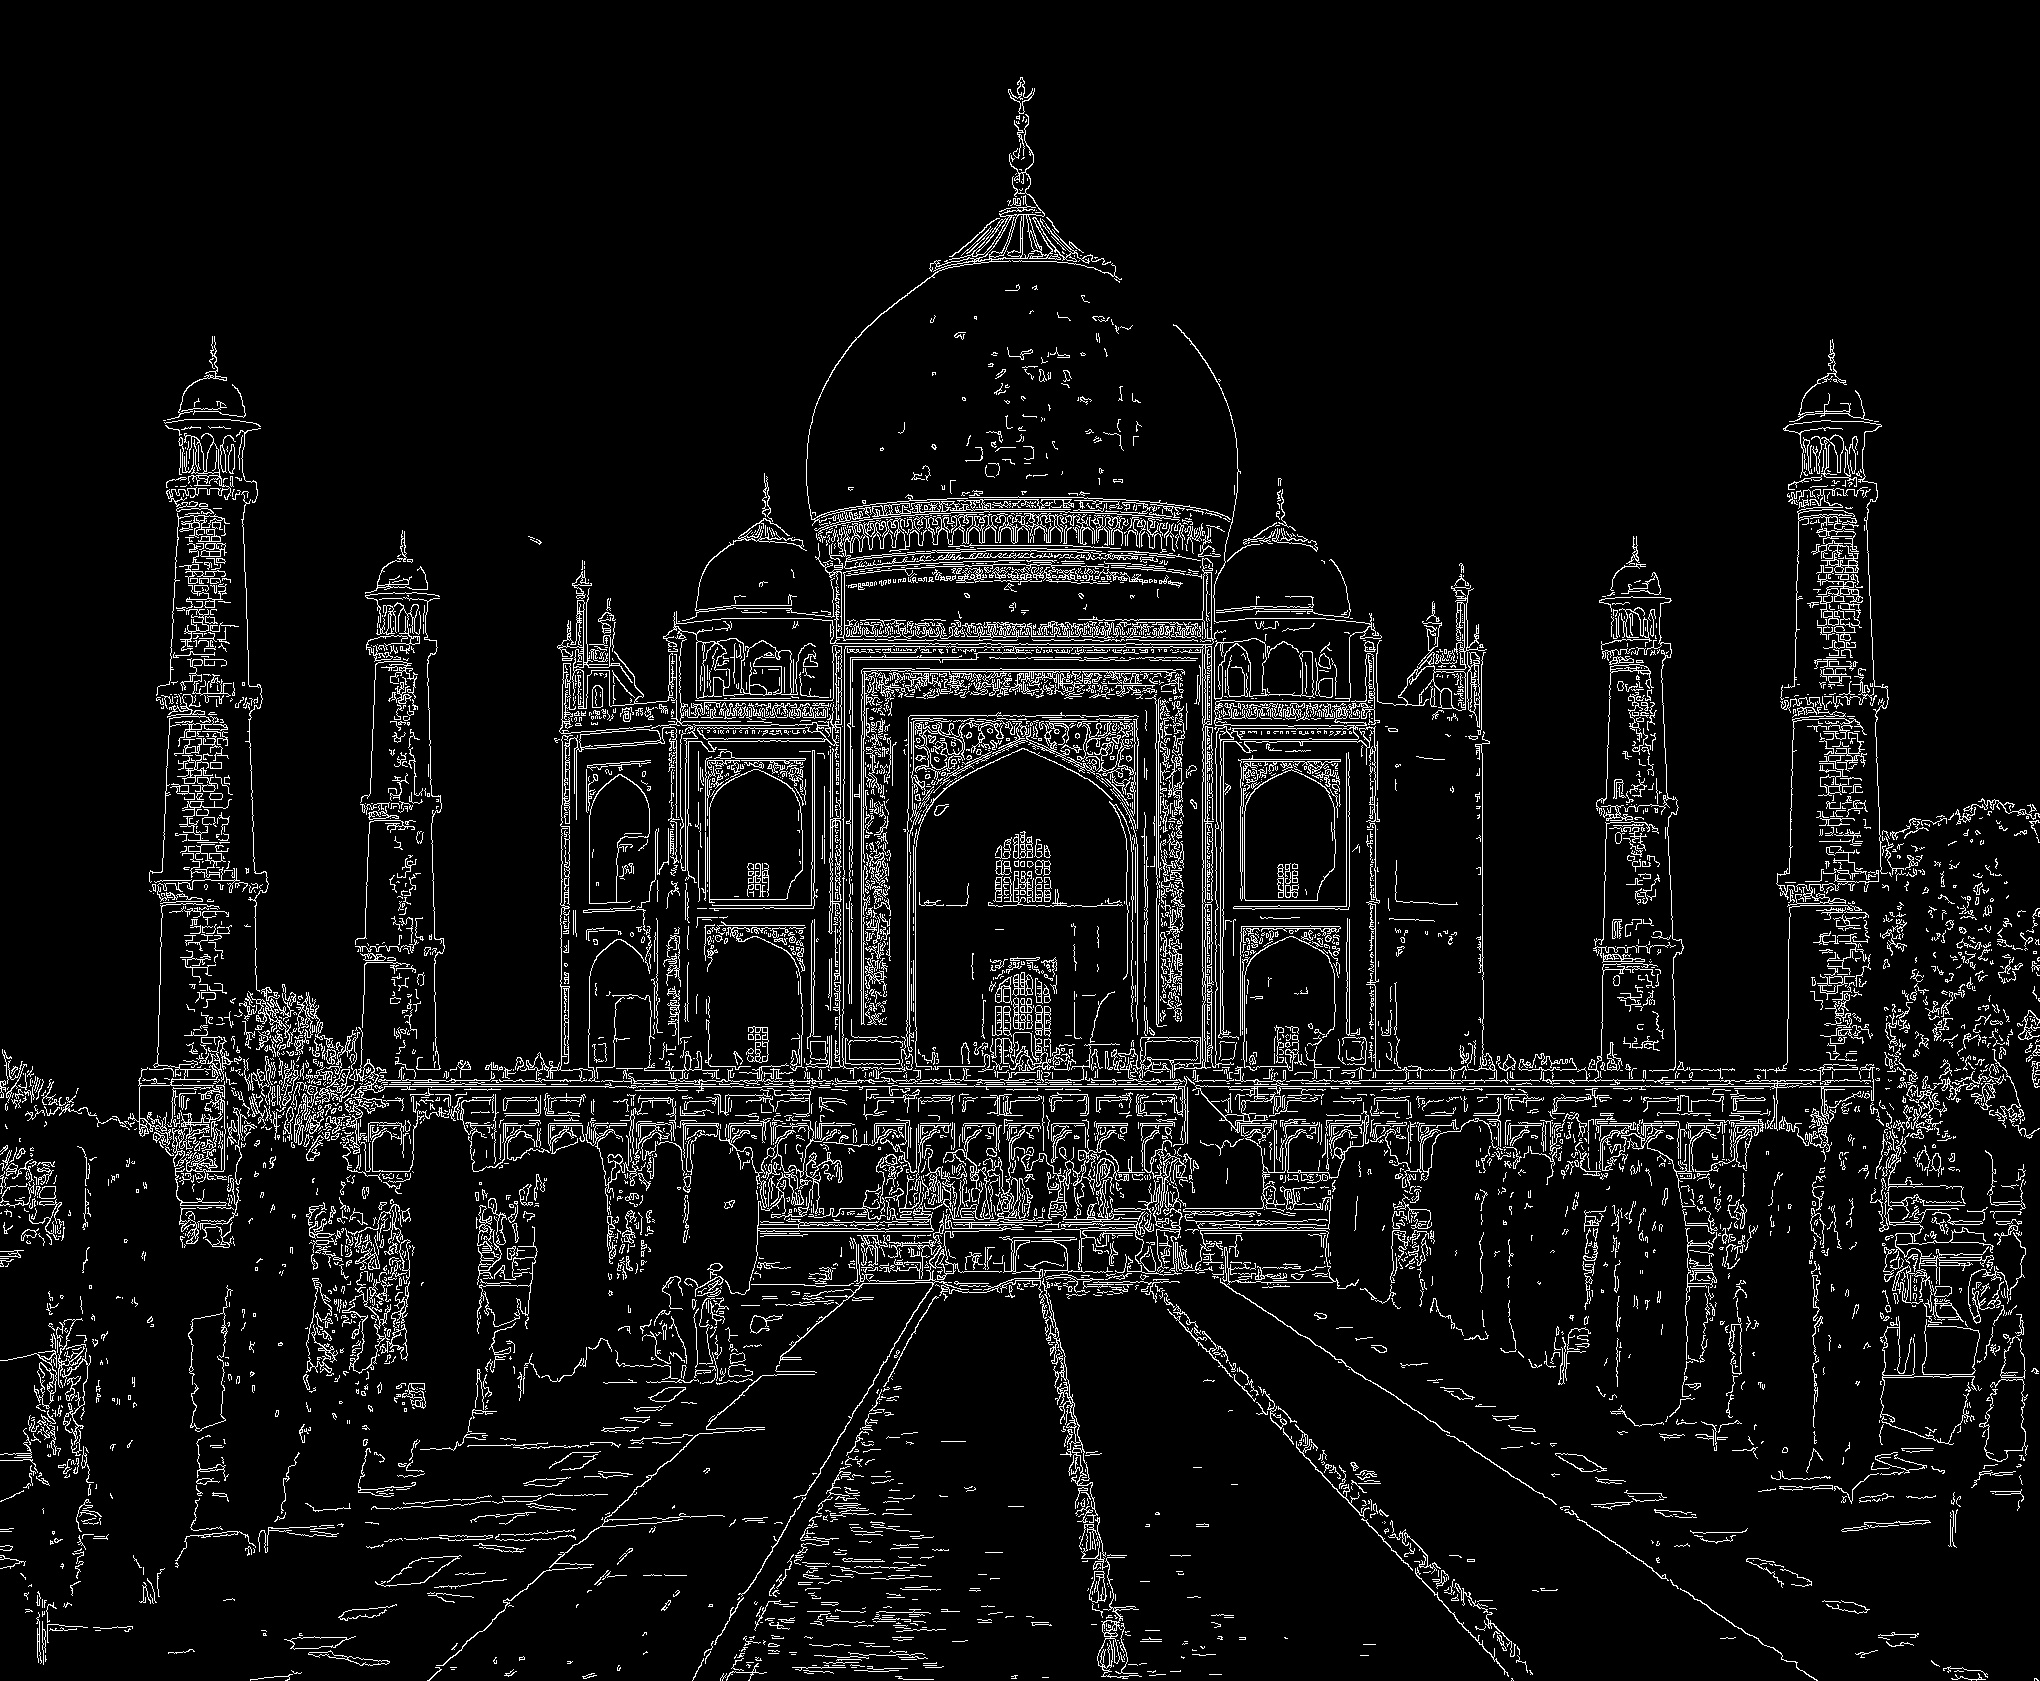
\includegraphics[width=20mm,scale=0.7]{images/taj_mahal_detectedges.jpg}};
		\node [below of = raw,anchor=north] (edge)  { \resizebox{15mm}{5mm}{ \begin{tabular}{ccccc}
			0 & 0  & 0  & 0  & 0   \\
			0 & 1 & 1 & 1  & 0   \\
			0 & 1 & -8  & 1 & 0  \\
			0 & 1  & 1 & 1  & 0   \\
			0 & 0  & 0  & 0  & 0  
			\end{tabular} }};
		\node[above of= raw,node distance=1.2cm ] (features)  {\footnotesize{Features}};
		\draw[->,thick] (input_taj) -- (raw) ;

	}
	\onslide<1->{\node [right=5cm of raw.center,anchor= center](output_taj){car, bus, \textcolor{blue}{monument}, flower};
		\draw[->,thick] (raw) -- (output_taj) ;
		\node [] (o) at ($(output_taj) + (0,1.2)$) {\footnotesize{Classifier}};
		\node [] (i) at ($(input_taj) + (0,1.2)$) {\footnotesize{Input}};
	}

\end{tikzpicture}
		\end{minipage}
		
		\begin{minipage}[t]{0.25\textwidth}
			\begin{tikzpicture}[scale=0.9,transform shape] 
	\onslide<2->{ \node[] (input_taj) 
		{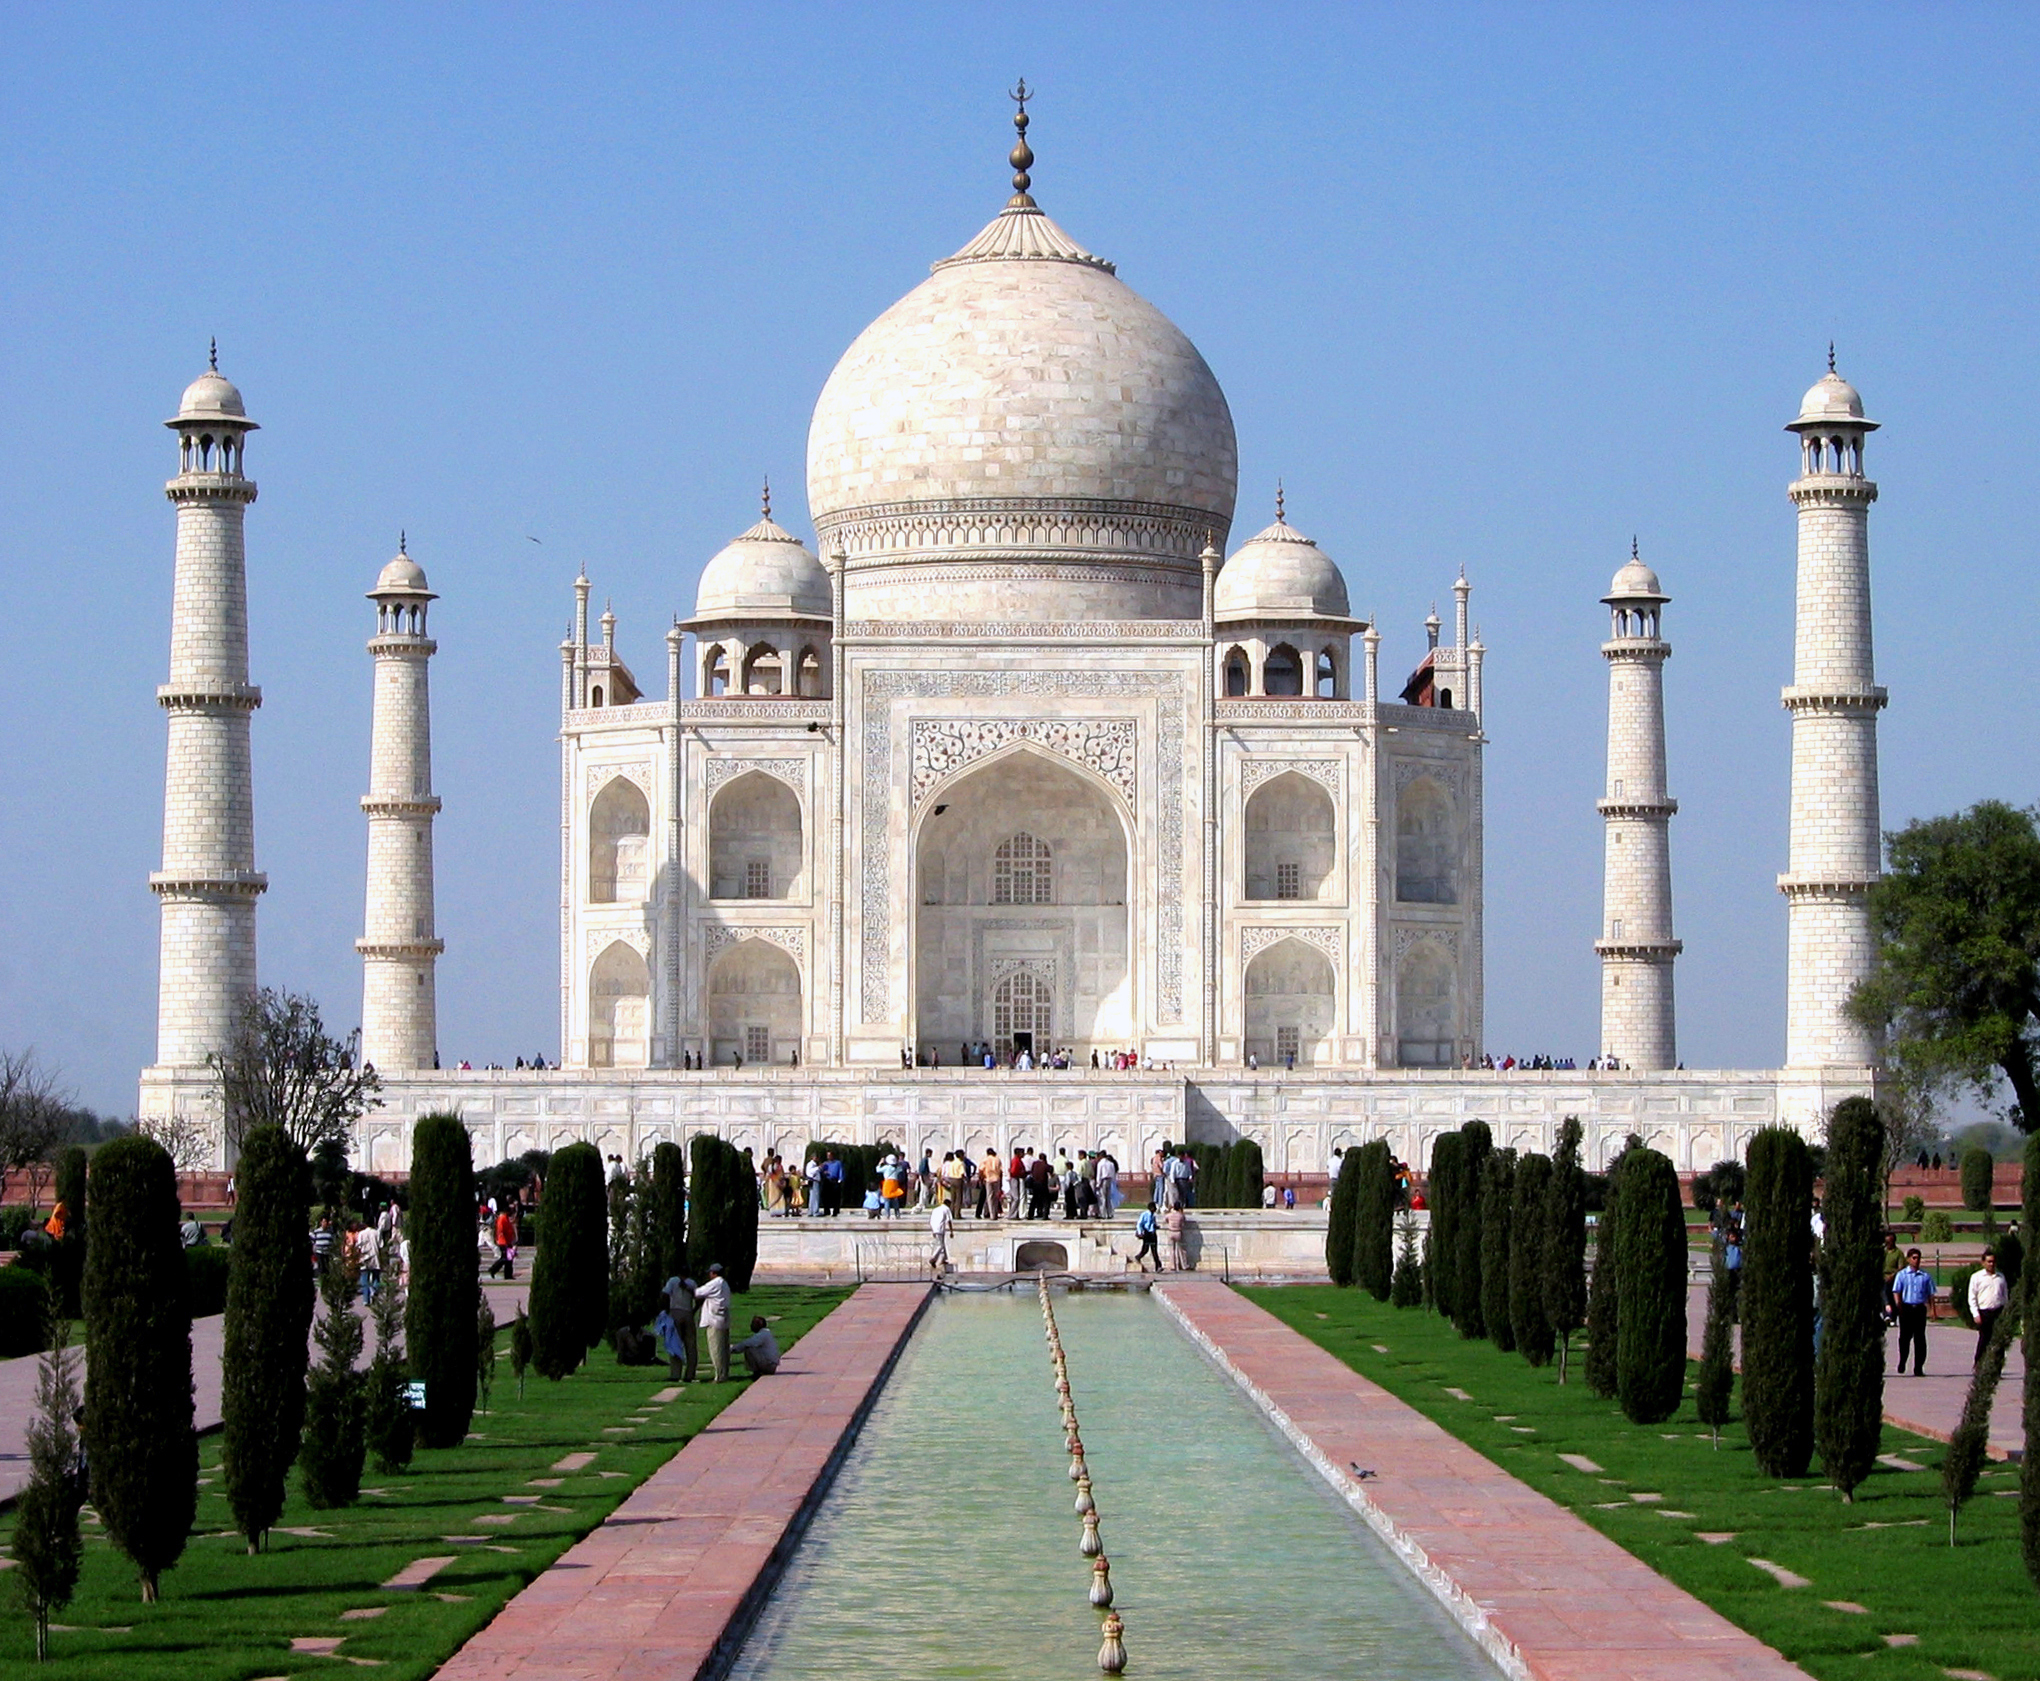
\includegraphics[width=20mm,height=17mm,scale=0.7]{images/taj_mahal.jpg}};
	}
	\onslide<2->{  \node (raw) at ($(input_taj) + (4,0)$)  { 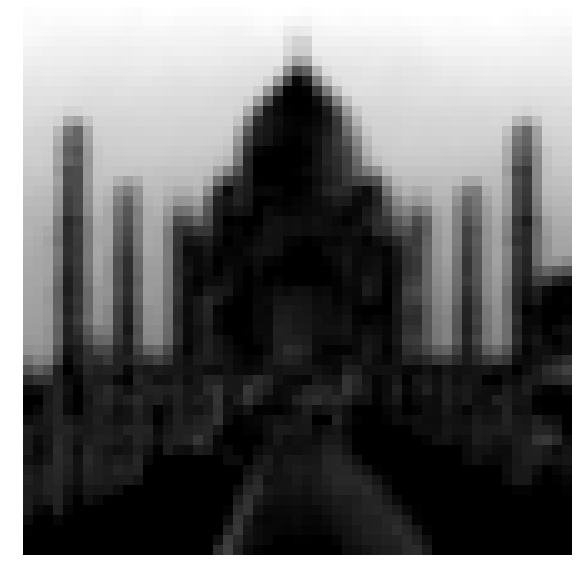
\includegraphics[width=20mm,height=17mm,scale=0.7]{images/convo1.png}};
		\node [below of = raw,anchor=north] (edge)  { \resizebox{25mm}{8mm}{ \begin{tabular}{ccccc}
			-1.21358689e-03  & 3.23652686e-03 & $\cdots$ & $\cdots$ & -2.06615720e-02\\ 
			-1.52757822e-03  & 2.36130832e-03 & $\cdots$ & $\cdots$ & -1.19824838e-02\\ 
			$\vdots$ & $\vdots$ &  &  & $\vdots$\\ 
			$\vdots$ & $\vdots$ &  &  & $\vdots$\\ 
			-8.25322699e-04 & -5.14897937e-03 &  $\cdots$ & $\cdots$ &-9.90395527e-03 \\
			\end{tabular} }};
		%\node[above of= raw,node distance=1.2cm ] (features)  {\footnotesize{Features}};
		\draw[->,thick] (input_taj) -- (raw) ;

	}
	\onslide<2->{\node(output_taj) at ($(input_taj) + (9,0)$) {car, bus, \textcolor{blue}{monument}, flower};
		\draw[->,thick] (raw) -- (output_taj) ;}
	
	\onslide<3->{\node [] (edge1) at ($(edge) + (5,0)$){{\textcolor{red}{Learn these weights}}};
		\draw [->, thick] (edge1) -- (edge);
	}

\end{tikzpicture}
		\end{minipage}
		
		\begin{minipage}[t]{\textwidth}
			\onslide<1->{
				\begin{itemize}
					\justifying
					\item \footnotesize{
					            Instead of using handcrafted kernels such as edge detectors \textbf{can we learn meaningful kernels/filters in addition to learning the weights of the classifier?}
					      }
				\end{itemize}
			}
		\end{minipage}
		
	\end{overlayarea}
\end{frame}



%%%%%%%%%%%%%%%%%%%%%%%%%%%%%%%%%%%%%%%%%%%%%%%%%%%%%%%%%%%%%%%%%%%%%%%%%%%%%%%%%%%%%%%%%
\begin{frame}
	\begin{overlayarea}{\textwidth}{\textheight}
		
		
		\begin{minipage}[t]{0.25\textwidth}
			\begin{tikzpicture}[scale=0.9,transform shape] 
	\onslide<1->{ \node[] (input_taj) 
		{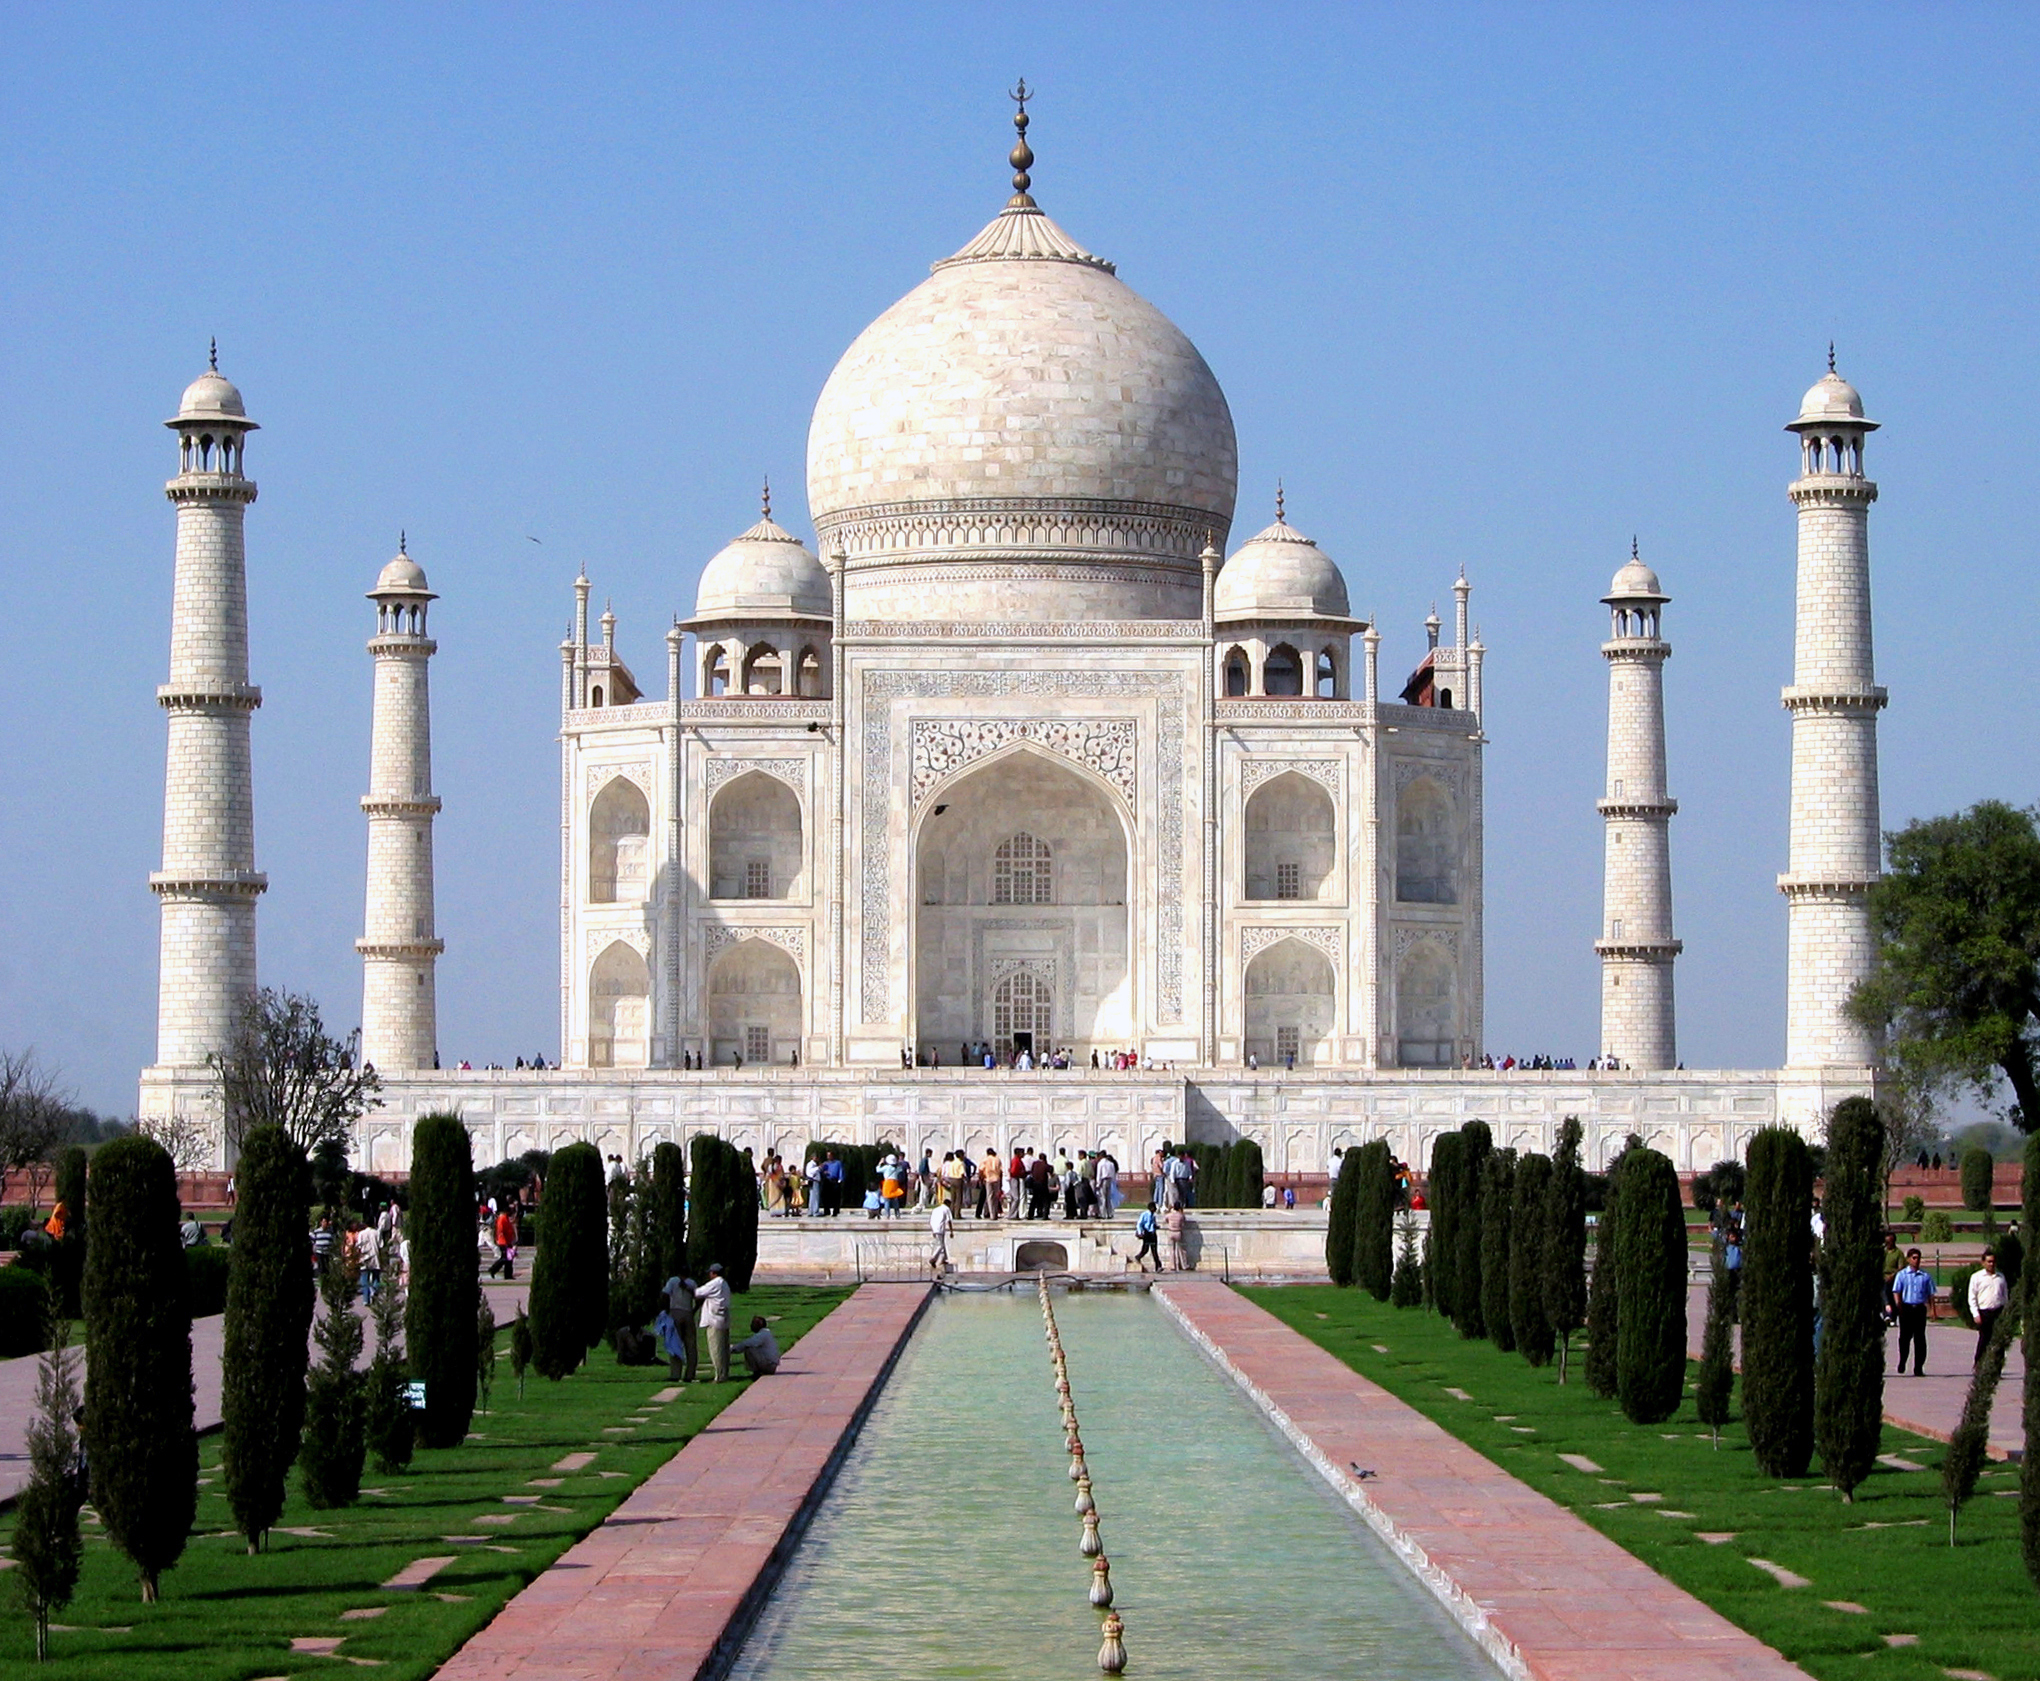
\includegraphics[width=20mm,scale=0.7]{images/taj_mahal.jpg}};
	}
	\onslide<1->{  \node [right=3cm of input_taj.south,anchor=south west] (raw)  { 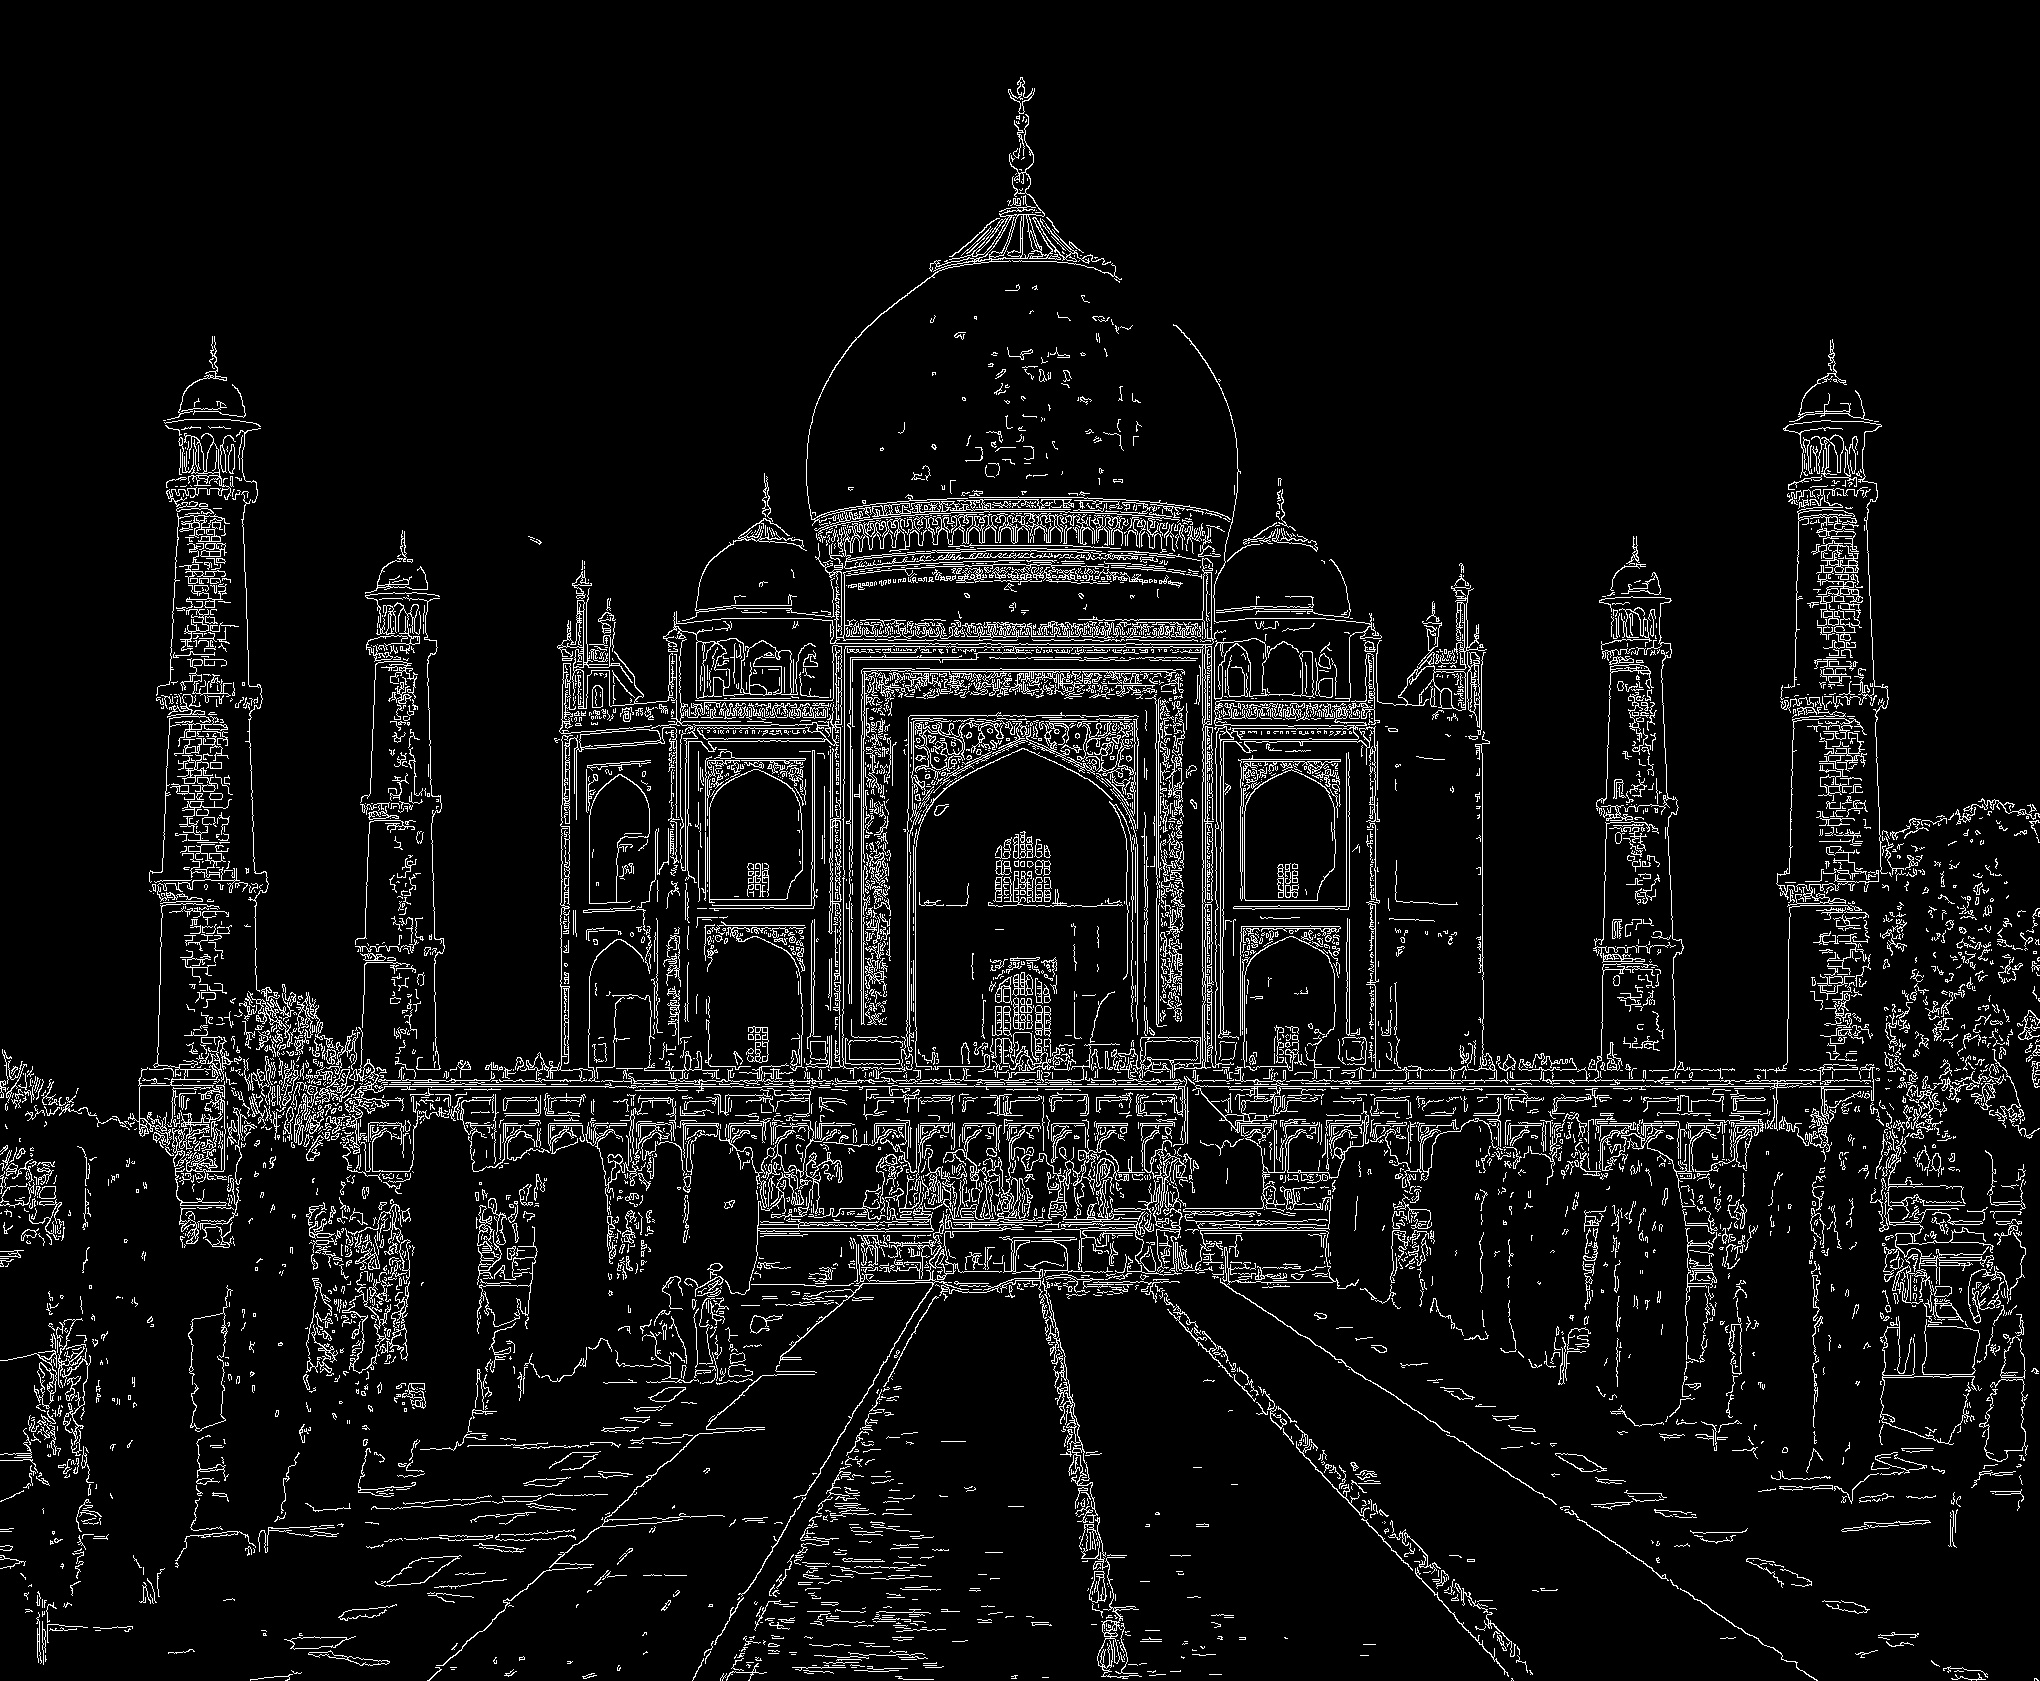
\includegraphics[width=20mm,scale=0.7]{images/taj_mahal_detectedges.jpg}};
		\node [below of = raw,anchor=north] (edge)  { \resizebox{15mm}{5mm}{ \begin{tabular}{ccccc}
			0 & 0  & 0  & 0  & 0   \\
			0 & 1 & 1 & 1  & 0   \\
			0 & 1 & -8  & 1 & 0  \\
			0 & 1  & 1 & 1  & 0   \\
			0 & 0  & 0  & 0  & 0  
			\end{tabular} }};
		\node[above of= raw,node distance=1.2cm ] (features)  {\footnotesize{Features}};
		\draw[->,thick] (input_taj) -- (raw) ;

	}
	\onslide<1->{\node [right=5cm of raw.center,anchor= center](output_taj){car, bus, \textcolor{blue}{monument}, flower};
		\draw[->,thick] (raw) -- (output_taj) ;
		\node [] (o) at ($(output_taj) + (0,1.2)$) {\footnotesize{Classifier}};
		\node [] (i) at ($(input_taj) + (0,1.2)$) {\footnotesize{Input}};
	}
\end{tikzpicture}
		\end{minipage}
		
		\begin{minipage}[t]{0.25\textwidth}
			\begin{tikzpicture} [scale=0.9, transform shape]
	\onslide<1->{ \node[] (input_taj) 
		{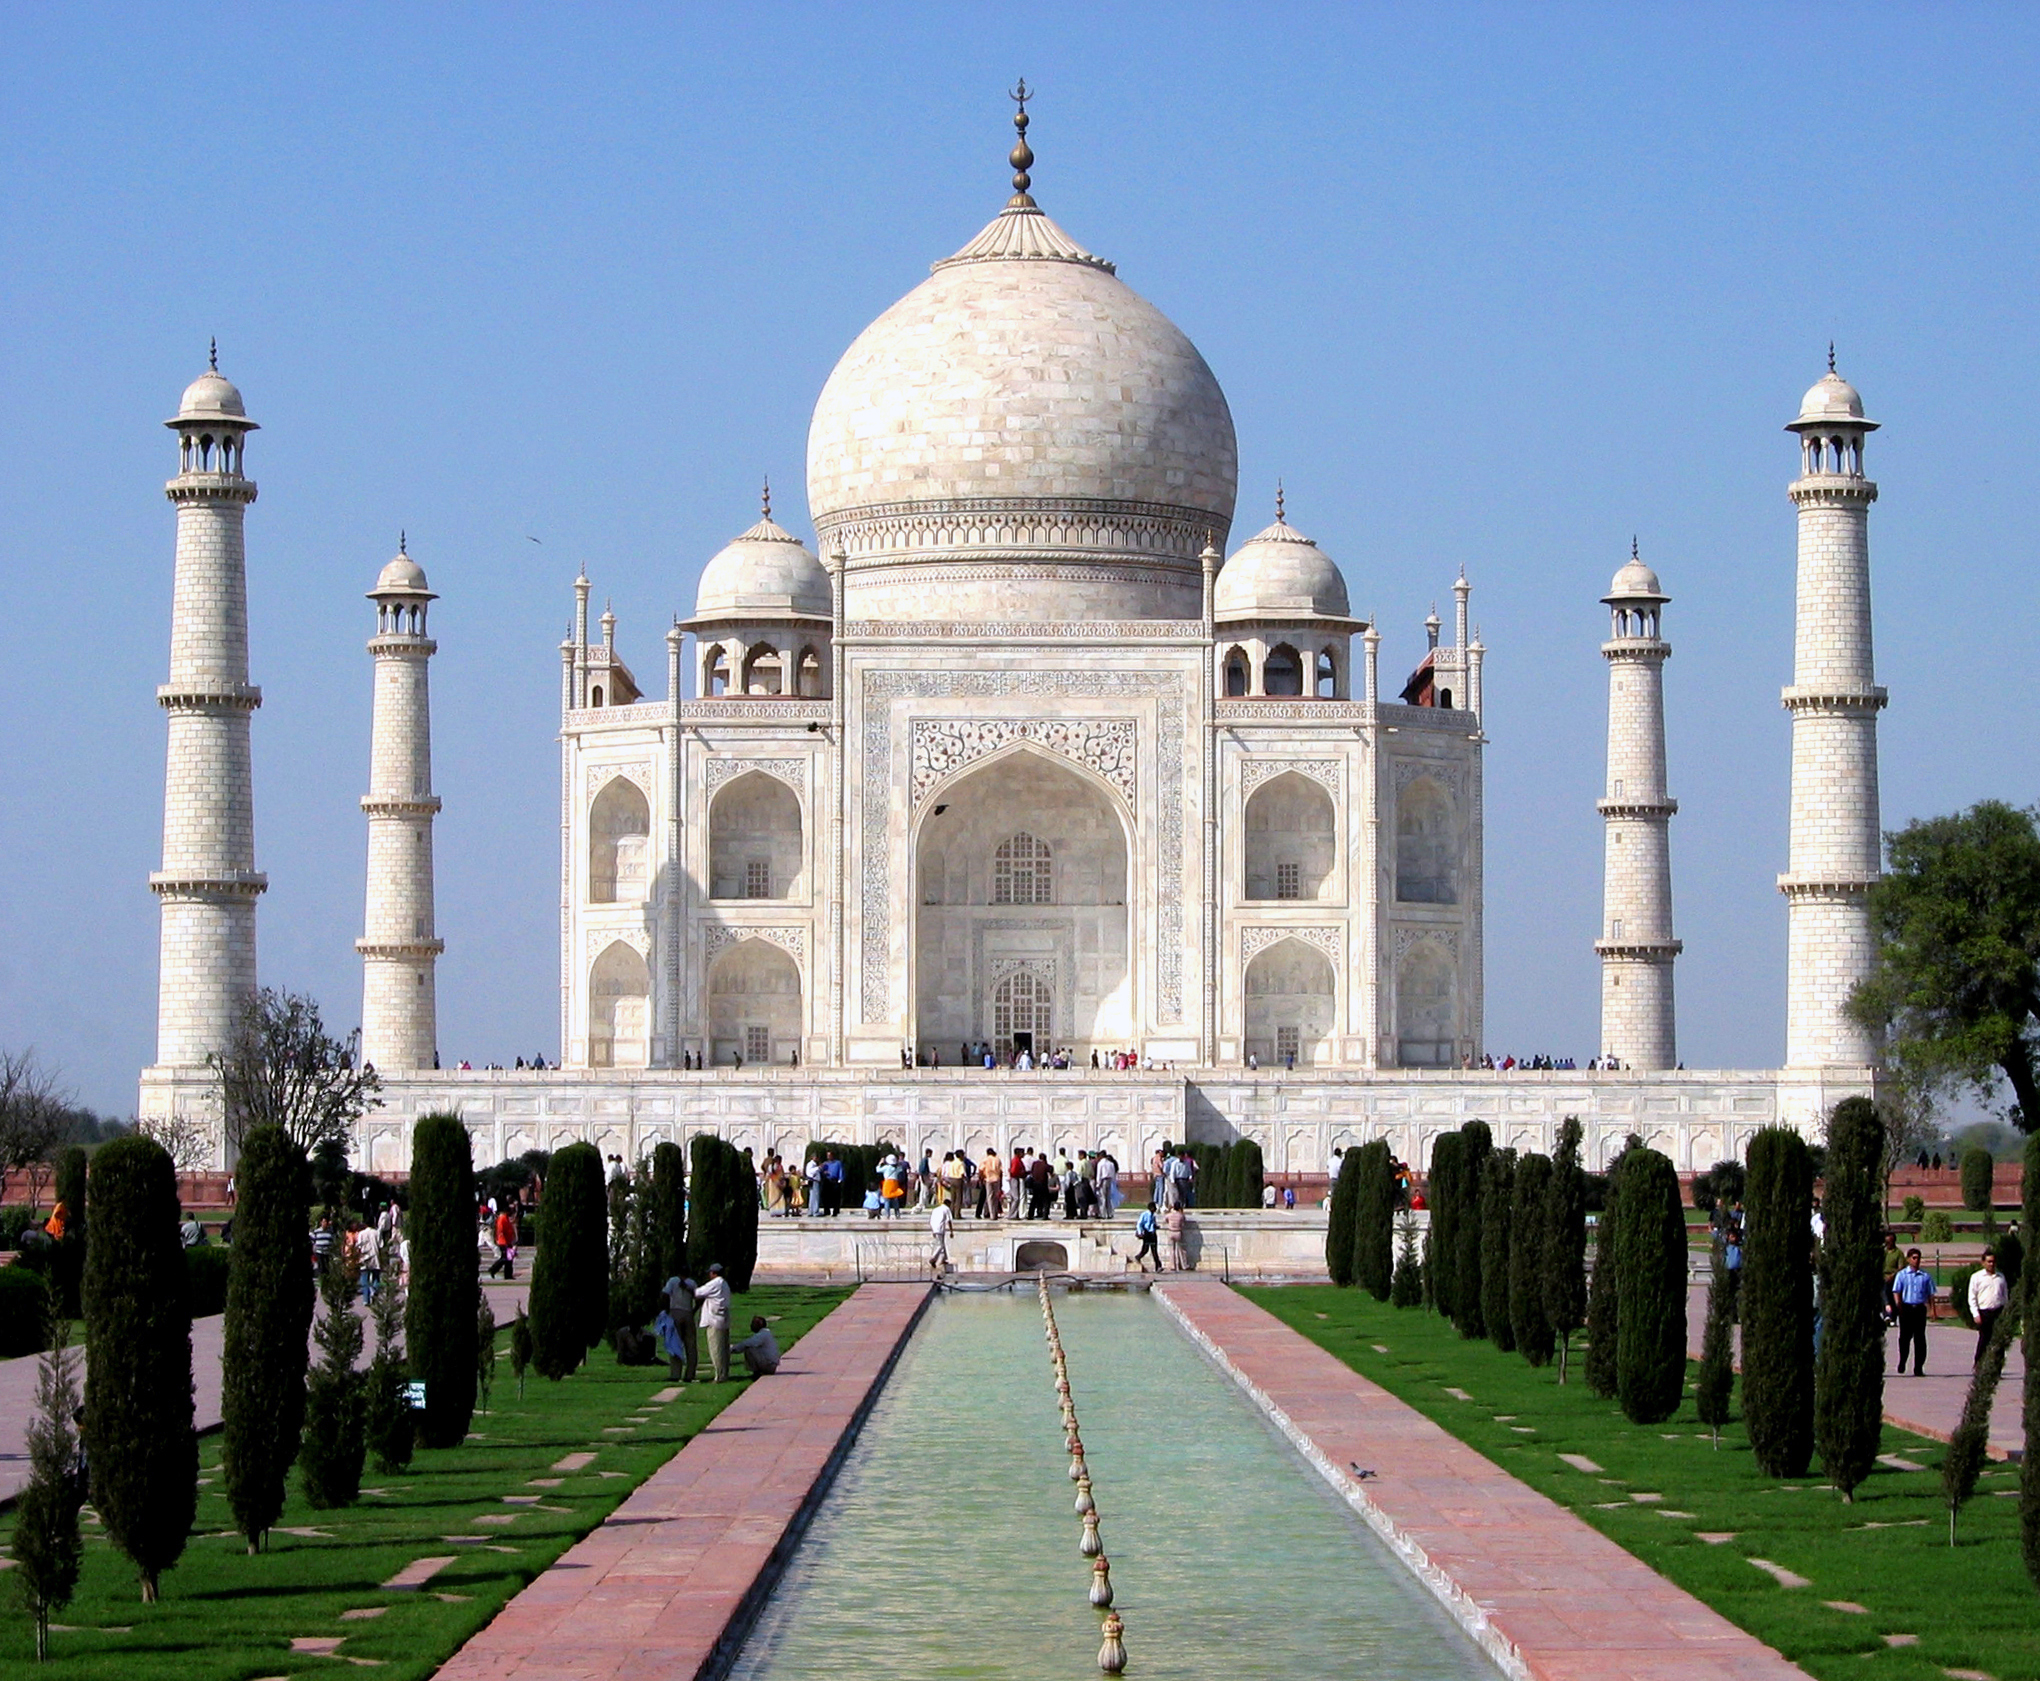
\includegraphics[width=20mm,height=17mm,scale=0.7]{images/taj_mahal.jpg}};
	}
	\onslide<1->{  \node (raw) at ($(input_taj) + (4, 0)$)  { 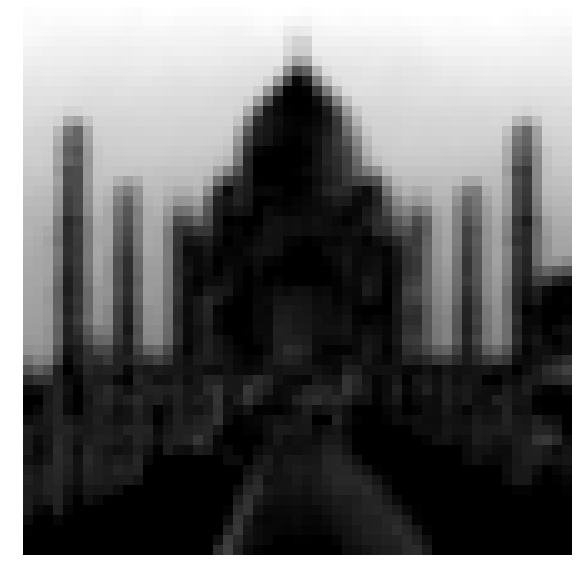
\includegraphics[width=20mm,height=17mm,scale=0.7]{images/convo1.png}};}
	\onslide<2->{\node (raw1) at ($(raw) + (0.2,0.2)$)  { 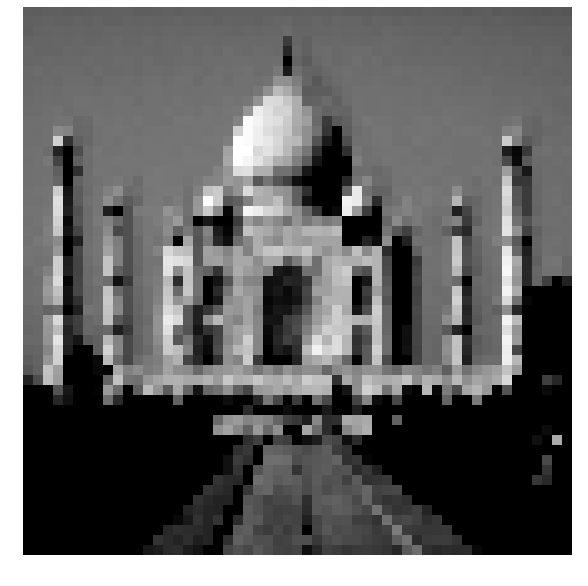
\includegraphics[width=20mm,height=17mm,scale=0.7]{images/convo1_49.png}};
	; }
	\onslide<3->{\node (raw2) at ($(raw1) + (0.2,0.2)$)  { 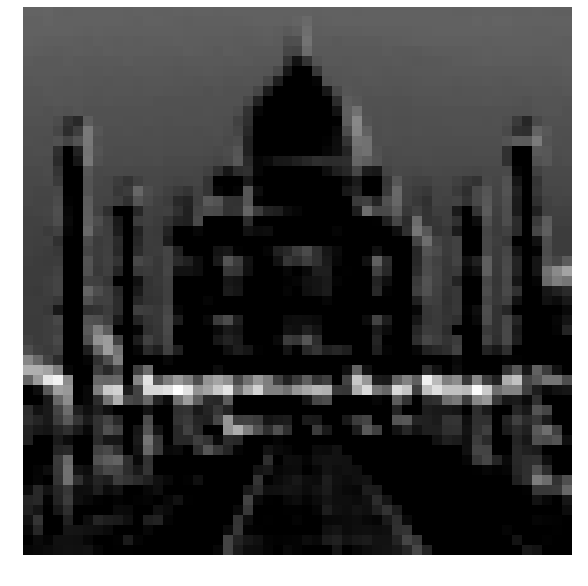
\includegraphics[width=20mm,height=17mm,scale=0.7]{images/convo1_74.png}}; }
	\onslide<1>{
		\node [below of = raw,anchor=north] (edge)  { \resizebox{25mm}{8mm}{ \begin{tabular}{ccccc}
			-1.21358689e-03  & 3.23652686e-03 & $\cdots$ & $\cdots$ & -2.06615720e-02\\ 
			-1.52757822e-03  & 2.36130832e-03 & $\cdots$ & $\cdots$ & -1.19824838e-02\\ 
			$\vdots$ & $\vdots$ &  &  & $\vdots$\\ 
			$\vdots$ & $\vdots$ &  &  & $\vdots$\\ 
			-8.25322699e-04 & -5.14897937e-03 &  $\cdots$ & $\cdots$ &-9.90395527e-03 \\
			\end{tabular} }};
		%\node[above of= raw,node distance=1.2cm ] (features)  {Features};
		\draw[->,thick] (input_taj) -- (raw) ;
	}
	\onslide<2>{ 
		\node [below of = raw,anchor=north] (edge)  { \resizebox{25mm}{8mm}{ \begin{tabular}{ccccc}
			-0.02337041 & -0.03243878 & $\cdots$ & $\cdots$ & -0.04728875\\ 
			-0.05375158 & -0.05350766 $\cdots$ & $\cdots$ & -0.04323674\\ 
			$\vdots$ & $\vdots$ &  &  & $\vdots$\\ 
			$\vdots$ & $\vdots$ &  &  & $\vdots$\\ 
			-0.00792501 & -0.00503319 &  $\cdots$ & $\cdots$ &0.00174674 \\
			\end{tabular} }};
		%\node[above of= raw,node distance=1.2cm ] (features)  {Features};
		\draw[->,thick] (input_taj) -- (raw) ;

	}
	\onslide<3->{
		\node [below of = raw,anchor=north] (edge)  { \resizebox{25mm}{8mm}{ \begin{tabular}{ccccc}
			-0.01871333 & -0.01075948 & $\cdots$ & $\cdots$ & 0.04684572\\ 
			0.00104325 & 0.01935937 & $\cdots$ & $\cdots$ & 0.01016542\\ 
			$\vdots$ & $\vdots$ &  &  & $\vdots$\\ 
			$\vdots$ & $\vdots$ &  &  & $\vdots$\\ 
			0.03008777 &  0.00335217 &  $\cdots$ & $\cdots$ &-0.02791128 \\
			\end{tabular} }};
		%\node[above of= raw,node distance=1.2cm ] (features)  {Features};
		\draw[->,thick] (input_taj) -- (raw) ;

	}
	\onslide<1->{\node [right=5cm of raw.center,anchor= center](output_taj){car, bus, \textcolor{blue}{monument}, flower};
		\draw[->,thick] (raw) -- (output_taj) ;}

\end{tikzpicture}
		\end{minipage}
		
		\begin{minipage}[t]{\textwidth}
			\onslide<1->{
				\vspace{-1.2em}
				\begin{itemize}
					\justifying
					\item \footnotesize{\textbf{Even better:} Instead of using handcrafted kernels (such as edge detectors)\textbf{can we learn \textcolor{red}{multiple} meaningful kernels/filters in addition to learning the weights of the classifier?}}
				\end{itemize}
			}
		\end{minipage}
		
	\end{overlayarea}
\end{frame}



%%%%%%%%%%%%%%%%%%%%%%%%%%%%%%%%%%%%%%%%%%%%%%%%%%%%%%%%%%%%%%%%%%%%%%%%%%%%%%%%%%%%%%%%%
%---------------------------------------------------------------------------------------------------------------------------------------------------------------
\begin{frame}
	\begin{overlayarea}{\textwidth}{\textheight}
		
		\begin{minipage}[t]{0.25\textwidth}
			\vspace{3mm}
			\begin{tikzpicture}[scale=0.8,transform shape]
	\onslide<2->{ \node[] (input_taj) 
		{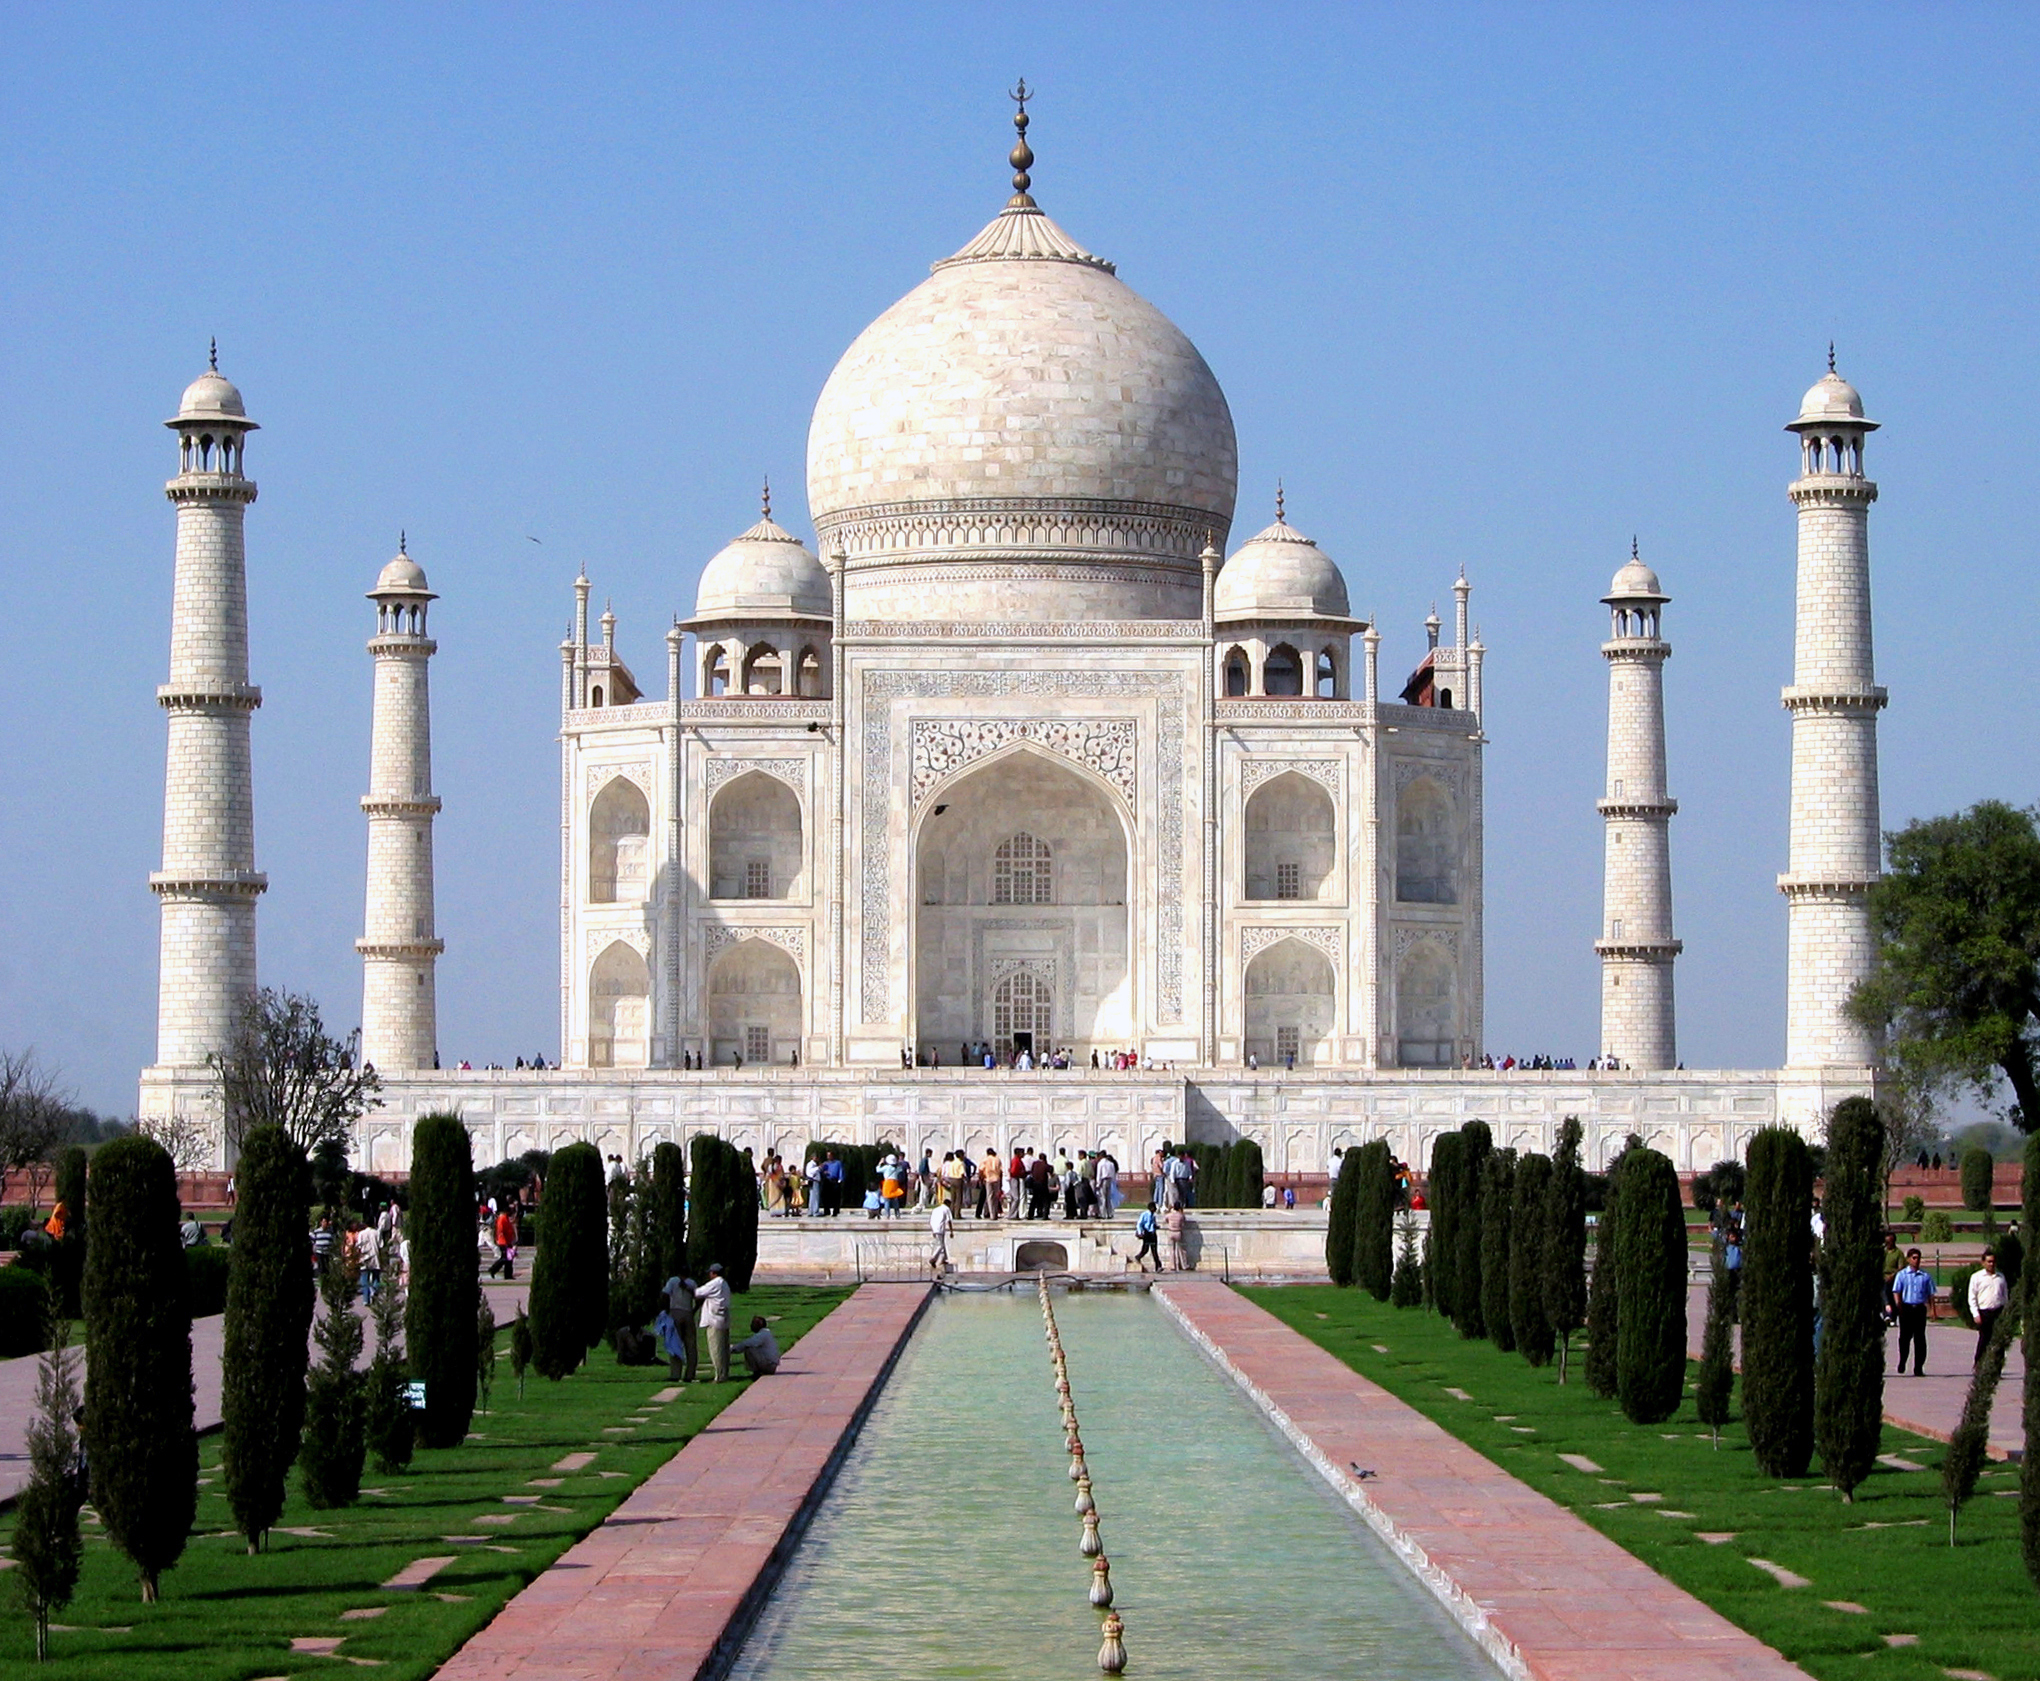
\includegraphics[width=20mm,height=17mm,scale=0.7]{images/taj_mahal.jpg}};}
	\onslide<2->{  
		\node  (raw1) at ($(input_taj) + (4.5,0)$) { 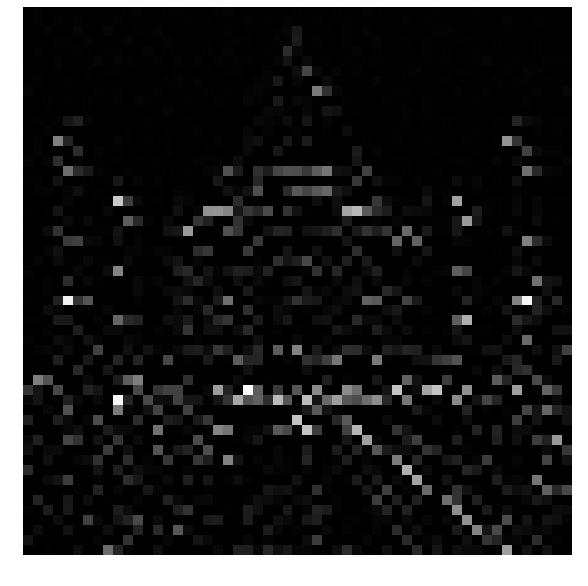
\includegraphics[width=20mm,height=17mm,scale=0.7]{images/convo1_2.png}};
		\node (raw2) at ($(raw1) + (-0.2,-0.2)$)  { 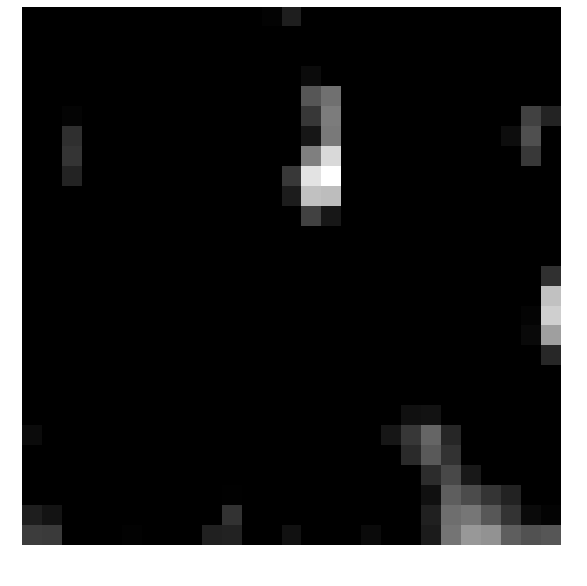
\includegraphics[width=20mm,height=17mm,scale=0.7]{images/convo2_2.png}};
		\node (raw3) at ($(raw2) + (-0.4,-0.2)$) { 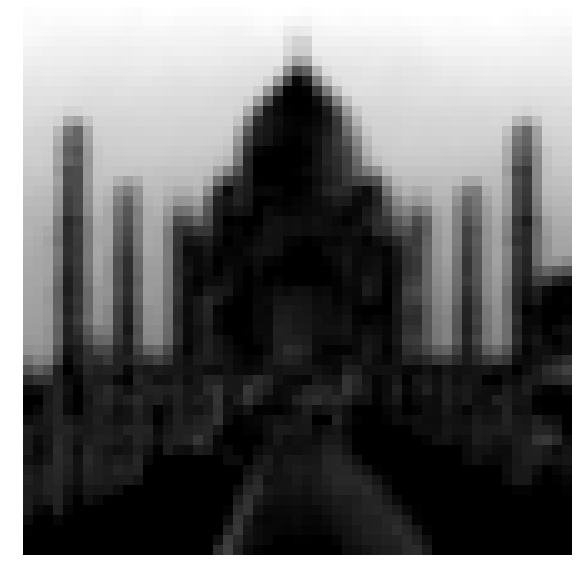
\includegraphics[width=20mm,height=17mm,scale=0.7]{images/convo1.png}};

		%\node[above of= raw,node distance=1.2cm ] (features)  {Features};
		\draw[->,thick] (input_taj) -- ($(raw1) + (-2,0)$) ;

	}
	\onslide<2->{

		\node (raw4) at ($(raw1) + (4.5,0)$)  { 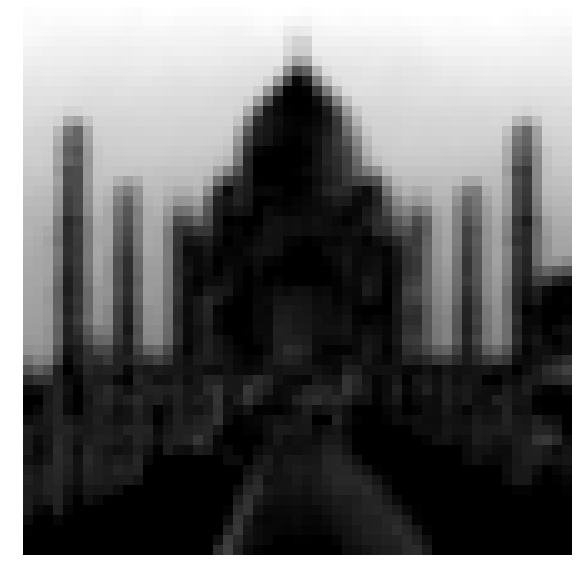
\includegraphics[width=20mm,height=17mm,scale=0.7]{images/convo1.png}};
		\node (raw5) at ($(raw4) + (-0.2,-0.2)$) { 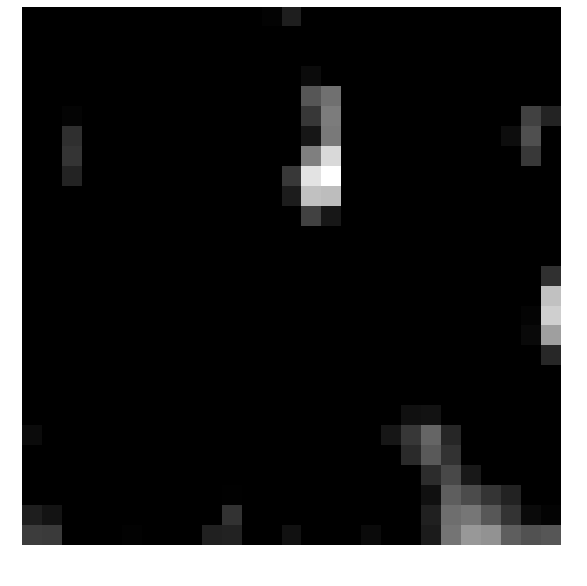
\includegraphics[width=20mm,height=17mm,scale=0.7]{images/convo2_2.png}};
		\node (raw6) at ($(raw5) + (-0.4,-0.2)$)  { 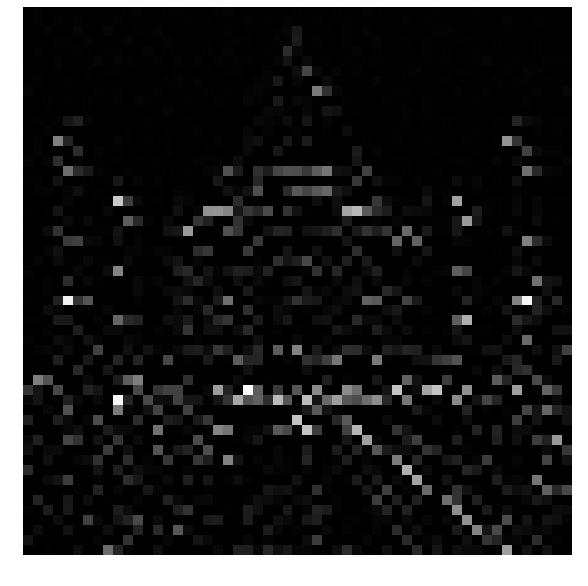
\includegraphics[width=20mm,height=17mm,scale=0.7]{images/convo1_2.png}};
		%\node[above of= raw,node distance=1.2cm ] (features)  {Features};

		\draw[->,thick] (raw1) -- ($(raw4) + (-2,0)$) ;
	}

	\onslide<2->{\node [right=4cm of raw4.center,anchor= center](output_taj){car, bus, \textcolor{blue}{monument}, flower};
		\draw[->,thick] (raw4) -- (output_taj) ;
		\node [] (o) at ($(output_taj) + (0,1.2)$) {\footnotesize{Classifier}};
		\node [] (i) at ($(input_taj) + (0,1.2)$) {\footnotesize{Input}};
	}


	\onslide<3->{\node [below of = output_taj,node distance=4.8em,anchor= center](back){\footnotesize{backpropagation}};
	}
	\onslide<3->{ 
		\node [below of = raw5,anchor=north] (edge2)  { \resizebox{25mm}{8mm}{ \begin{tabular}{ccccc}
			-0.01112582  & 0.02185669 & $\cdots$ & $\cdots$ & 0.00015161\\ 
			-0.00687587 & 0.01229961 & $\cdots$ & $\cdots$ & 0.00214013\\ 
			$\vdots$ & $\vdots$ &  &  & $\vdots$\\ 
			$\vdots$ & $\vdots$ &  &  & $\vdots$\\ 
			-0.00372989 & -0.00886137  &  $\cdots$ & $\cdots$ &-0.01974954 \\
			\end{tabular} }};
 
		\draw[->,thick] (back) -- ($(edge2) + (1.5,0.25)$) ;
	}
	\onslide<3->{
		\node [below of = raw2,anchor=north] (edge1)  { \resizebox{25mm}{8mm}{ \begin{tabular}{ccccc}
			-1.21358689e-03  & 3.23652686e-03 & $\cdots$ & $\cdots$ & -2.06615720e-02\\ 
			-1.52757822e-03  & 2.36130832e-03 & $\cdots$ & $\cdots$ & -1.19824838e-02\\ 
			$\vdots$ & $\vdots$ &  &  & $\vdots$\\ 
			$\vdots$ & $\vdots$ &  &  & $\vdots$\\ 
			-8.25322699e-04 & -5.14897937e-03 &  $\cdots$ & $\cdots$ &-9.90395527e-03 \\
			\end{tabular} }};
		\draw[->,thick] (edge2) -- (edge1) ;   
	}


\end{tikzpicture}
		\end{minipage}
		
		\begin{minipage}[t]{\textwidth}
			\vspace{6mm}
			\small{
				\begin{itemize}
					\justifying
					\item <1-> \textbf{Can we learn multiple \textcolor{red}{layers} of meaningful kernels/filters in addition to learning the weights of the classifier? }
					\item <2-> Yes, we can ! 
					\item <3-> Simply by treating these kernels as parameters and learning them in addition to the weights of the classifier (using back propagation)
					\item <4-> Such a network is called a Convolutional Neural Network.
				\end{itemize}
			}
			
			    
		\end{minipage}
		
	\end{overlayarea}
\end{frame}


%%%%%%%%%%%%%%%%%%%%%%%%%%%%%%%%%%%%%%%%%%%%%%%%%%%%%%%%%%%%%%%%%%%%%%%%%%%%%%%%%%%%%%%%%
\begin{frame}
	\begin{block}{}
		\onslide<1-3>{
			\begin{itemize}
				\justifying
				\item <1-> Okay, I get it that the idea is to learn the kernel/filters by just treating them as parameters of the classification
				      model
				      \item<2-> But how is this different from a regular feedforward neural network
				      \item<3-> Let us see
			\end{itemize}}
	\end{block}
\end{frame}


%%%%%%%%%%%%%%%%%%%%%%%%%%%%%%%%%%%%%%%%%%%%%%%%%%%%%%%%%%%%%%%%%%%%%%%%%%%%%%%%%%%%%%%%%

\begin{frame}
	\begin{columns}
		\begin{column}{0.5\textwidth}
			\begin{tikzpicture}[square/.style={regular polygon,regular polygon sides=4}]
	\scriptsize
	% % 16 nodes with labels (1 to 16)
	\onslide<2->{
	\foreach \i in {1,...,16}
	{
	
	\pgfmathtruncatemacro{\label}{\i};
	\node[square,draw=red!50,fill=orange!10,thick,minimum size=.2mm] (\label) at (-1*\i*0.5,-3) {};
	}
	% %Underbrace
	\draw [
	thick,
	decoration={
	brace,
	raise=0.5cm
	},
	decorate
	] (1) -- (16) 
	node [pos=0.5,anchor=south,yshift=-1.1cm] {16}; }
	
	%%Grid
	
	\onslide<1->{\draw[step=0.25cm,gray,very thin] (-4.75,-5.5) grid (-3.75,-4.5);
	\node[] at (-4.25,-5) {\Huge{2}};}
	% % %
	% % %  Layer 2
	\onslide<4->{	\foreach \i in {17,...,28}
	{
	\pgfmathtruncatemacro{\x}{(\i-14)};
	\pgfmathtruncatemacro{\label}{\i};
	\node[square,draw=blue!50,fill=blue!10,thick,minimum size=1mm] (\label) at (-1*\x*0.5,-2) {};
	}}
	% % %
	
	% % % Layer 3
	\onslide<5->{	\foreach \i in {29,...,36}
	{
		\pgfmathtruncatemacro{\x}{(\i-24)};
		\pgfmathtruncatemacro{\label}{\i};
		\node[square,draw=blue!50,fill=blue!10,thick,minimum size=1mm] (\label) at (-1*\x*0.5,-1) {};
	}}
	% % % 
	\onslide<6->{	\path (-4.15,-0.9) -- (-4.15,0.9) node [red, font=\Huge, midway, sloped] {$\dots$};}
	% % % Output Layer
	\onslide<3->{
		\foreach \i in {37,...,47}
		{
			\pgfmathtruncatemacro{\x}{(\i-35)};
			\pgfmathtruncatemacro{\label}{\i};
			\node[square,draw=green!50,fill=green!20,thick,minimum size=1mm] (\label) at (-1*\x*0.6,1) {};
		}
		% % %
		\draw [
		thick,
		decoration={
			brace,
			mirror,
			raise=0.5cm
		},
		decorate
		] (37) -- (47) 
		node [pos=0.5,anchor=north,yshift=1cm] {10 classes(digits)}; 
	}
	% %small circle h_11
	\onslide<7->{	\node[draw,circle,minimum size=0.5cm,inner sep=0pt] (cir) at (-7,-2) {};
	}
	% % connections layer 1
	\onslide<8->{	
		\foreach \from in {1,...,16}
		\foreach \to in {cir}
		\draw [->,draw=black!50] (\from) -- (\to);}
	
	
	\onslide<9->
	{
		\foreach \from in {17,...,28}
		\foreach \to in {29,...,36}
		\draw [->,draw=black!50] (\from) -- (\to);}
	
%\node[red,thick,dashed] (-7,-2) circle (0.3cm);
\end{tikzpicture}
		\end{column}
		\begin{column}{0.5\textwidth}
			
			\begin{itemize}
				%\justifying
				\setlength\itemsep{1em}
				\item<10-> This is what a regular feed-forward neural network will look like
				\item<11-> There are many dense connections here
				\item<12-> For example all the 16 input neurons are contributing to the computation of $h_{11}$
				\item<13-> Contrast this to what happens in the case of convolution
			\end{itemize}
		\end{column}
	\end{columns}
\end{frame}

%%%%%%%%%%%%%%%%%%%%%%%%%%%%%%%%%%%%%%%%%%%%%%%%%%%%%%%%%%%%%%%%%%%%%%%%%%%%%%%%%%%%%%%%%

\begin{frame}
	\begin{columns}
		\begin{column}{0.5\textwidth}
			\begin{overprint}
				\begin{tikzpicture}[square/.style={regular polygon,regular polygon sides=4}]
	%\begin{axis}[xlabel=x axis label,ylabel=y axis label]
    
	\onslide<1->{
		\foreach \i in {1,...,9}
		{
              
			\pgfmathtruncatemacro{\label}{\i};
			\node[square,draw=red!50,fill=orange!10,thick,minimum size=.2mm] (\label) at (-1*\i*0.5,-3) {};
		}
		\node[square,draw=red!50,fill=orange!10,thick,minimum size=.2mm] (10) at (1,-3) {};
		\path (1) -- node [red, font=\Huge, midway, sloped]{$\dots$} (10);
		%\end{axis}
         
		\draw [
			thick,
			decoration={
				brace,
				mirror,
				raise=0.5cm
			},
			decorate
		] (9) -- (10)
		node [pos=0.5,anchor=south,yshift=-1.1cm] {16};
		%\end{tikzpicture}
         
		%\begin{tikzpicture}[square/.style={regular polygon,regular polygon sides=4}]
		%% Grid 4
		\begin{scope}[scale=2.5,transform shape]
			\node[opacity=0.3] at (-1.17,-2.45) {\Huge{2}};
		\end{scope}
		\draw[step=0.5cm,gray,very thin] (-4,-7) grid (-2,-5);
		\node[] at (-1.5,-6) {*};
         
		\draw[step=0.5cm,gray,very thin] (-1,-6.50) grid (0,-5.5) ;
		\node[] at (0.5,-6) {=};
		%   \node[] at (1,-5.5) {$h_{11}$};
		\node[square,draw=blue!50,fill=blue!10,thick,minimum size=1mm] (1) at (1,-6) {};
     
		%% first row
		\node[circle,fill=\firstrowcolor,inner sep=0pt,minimum size=5.5pt](A) at (-3.75,-5.25   ) {};
		\node[circle,fill=\firstrowcolor,inner sep=0pt,minimum size=5.5pt](B) at (-3.75+0.5,-5.25   ) {};
     
		\node[circle,fill=\secondrowcolor,inner sep=0pt,minimum size=5.5pt](C) at (-3.75+2*0.5,-5.25    ) {};
		\node[circle,fill=\secondrowcolor,inner sep=0pt,minimum size=5.5pt](D) at (-3.75+3*0.5,-5.25    ) {};
     
		%% second row
		\node[circle,fill=\firstrowcolor,inner sep=0pt,minimum size=5.5pt](F) at (-3.75+0.5,-5.25-0.5   ) {};
		\node[circle,fill=\firstrowcolor,inner sep=0pt,minimum size=5.5pt](E) at (-3.75,-5.25-0.5   ) {};
		\node[circle,fill=\secondrowcolor,inner sep=0pt,minimum size=5.5pt](G) at (-3.75+2*0.5,-5.25-0.5    ) {};
		\node[circle,fill=\secondrowcolor,inner sep=0pt,minimum size=5.5pt](H) at (-3.75+3*0.5,-5.25-0.5    ) {};
     
		%% 3rd row
		\node[circle,fill=\thirdrowcolor,inner sep=0pt,minimum size=5.5pt](J) at (-3.75+0.5,-5.25-2*0.5 ) {};
		\node[circle,fill=\thirdrowcolor,inner sep=0pt,minimum size=5.5pt](I) at (-3.75,-5.25-2*0.5 ) {};
		\node[circle,fill=\fourrowcolor,inner sep=0pt,minimum size=5.5pt](K) at (-3.75+2*0.5,-5.25-2*0.5    ) {};
		\node[circle,fill=\fourrowcolor,inner sep=0pt,minimum size=5.5pt](L) at (-3.75+3*0.5,-5.25-2*0.5    ) {};
     
		%% 4th row
     
		\node[circle,fill=\thirdrowcolor,inner sep=0pt,minimum size=5.5pt](N) at (-3.75+0.5,-5.25-3*0.5 ) {};
		\node[circle,fill=\thirdrowcolor,inner sep=0pt,minimum size=5.5pt](M) at (-3.75,-5.25-3*0.5 ) {};
		\node[circle,fill=\fourrowcolor,inner sep=0pt,minimum size=5.5pt](O) at (-3.75+3*0.5,-5.25-3*0.5    ) {};
		\node[circle,fill=\fourrowcolor,inner sep=0pt,minimum size=5.5pt](P) at (-3.75+2*0.5,-5.25-3*0.5    ) {};
     
     
		\node[circle,fill=blue,inner sep=0pt,minimum size=5.5pt](Ai) at (-0.75,-5.75    ) {};
     
		\node[circle,fill=blue,inner sep=0pt,minimum size=5.5pt](Bi) at (-0.75+0.5,-5.75    ) {};
     
		\node[circle,fill=blue,inner sep=0pt,minimum size=5.5pt](Bi) at (-0.75,-5.75-0.5    ) {};
     
		\node[circle,fill=blue,inner sep=0pt,minimum size=5.5pt](Bi) at (-0.75+0.5,-5.75-0.5    ) {};
     
	}




	\onslide<3>{
     
		\renewcommand{\firstrowcolor}{red}
		\renewcommand{\secondrowcolor}{black}
		\renewcommand{\thirdrowcolor}{black}
		\renewcommand{\fourrowcolor}{black}
		\node[circle,fill=\firstrowcolor,inner sep=0pt,minimum size=5.5pt](A) at (-3.75,-5.25   ) {};
		\node[circle,fill=\firstrowcolor,inner sep=0pt,minimum size=5.5pt](B) at (-3.75+0.5,-5.25   ) {};
		\node[circle,fill=\firstrowcolor,inner sep=0pt,minimum size=5.5pt](F) at (-3.75+0.5,-5.25-0.5   ) {};
		\node[circle,fill=\firstrowcolor,inner sep=0pt,minimum size=5.5pt](E) at (-3.75,-5.25-0.5   ) {};
     
		\node[] at (1,-5.5) {$h_{11}$};s
     
     
		\node[circle,fill=blue,inner sep=0pt,minimum size=5.5pt](Ai) at (-0.75,-5.75    ) {};
     
		%% above animation
     
     
	}

	\onslide<3->{
		\node[square,draw=blue!50,fill=blue!10,thick,minimum size=1mm] (11) at (-3.25,-1.5) {};
     
		\foreach \i in {9,8,5,4}
		{
			\draw [-,draw=black!50] (\i) -- (11);
		}
		\node[] at (-3.25,-1.1) {$h_{11}$};
     
     
	}

	\only<4>{
     
		\renewcommand{\firstrowcolor}{black}
		\renewcommand{\secondrowcolor}{red}
		\renewcommand{\thirdrowcolor}{black}
		\renewcommand{\fourrowcolor}{black}
		\node[circle,fill=\secondrowcolor,inner sep=0pt,minimum size=5.5pt](G) at (-3.75+2*0.5,-5.25-0.5    ) {};
		\node[circle,fill=\secondrowcolor,inner sep=0pt,minimum size=5.5pt](H) at (-3.75+3*0.5,-5.25-0.5    ) {};
     
		\node[circle,fill=\secondrowcolor,inner sep=0pt,minimum size=5.5pt](C) at (-3.75+2*0.5,-5.25    ) {};
		\node[circle,fill=\secondrowcolor,inner sep=0pt,minimum size=5.5pt](D) at (-3.75+3*0.5,-5.25    ) {};
     
		\node[] at (1,-5.5) {$h_{12}$};
     
		\node[circle,fill=blue,inner sep=0pt,minimum size=5.5pt](Ai) at (-0.75,-5.75    ) {};
     
		\node[circle,fill=blue,inner sep=0pt,minimum size=5.5pt](Bi) at (-0.75+0.5,-5.75    ) {};
     
		%% above animation
     
     
     
     
		\node[] at (1,-5.5) {$h_{12}$};
     
     
	}
	\onslide<4->{
		\node[] at (-2.25,-1.1) {$h_{12}$};
		\node[square,draw=blue!50,fill=blue!10,thick,minimum size=1mm] (12) at (-2.25,-1.5) {};
		\foreach \i in {7,6,3,2}
		{
			\draw [-,draw=black!50] (\i) -- (12);
		}
	}

	\only<5>{
     
     
		\renewcommand{\firstrowcolor}{black}
		\renewcommand{\secondrowcolor}{black}
		\renewcommand{\thirdrowcolor}{red}
		\renewcommand{\fourrowcolor}{black}
     
		\node[circle,fill=\thirdrowcolor,inner sep=0pt,minimum size=5.5pt](J) at (-3.75+0.5,-5.25-2*0.5 ) {};
		\node[circle,fill=\thirdrowcolor,inner sep=0pt,minimum size=5.5pt](I) at (-3.75,-5.25-2*0.5 ) {};
     
		\node[circle,fill=\thirdrowcolor,inner sep=0pt,minimum size=5.5pt](N) at (-3.75+0.5,-5.25-3*0.5 ) {};
		\node[circle,fill=\thirdrowcolor,inner sep=0pt,minimum size=5.5pt](M) at (-3.75,-5.25-3*0.5 ) {};
		\node[circle,fill=blue,inner sep=0pt,minimum size=5.5pt](Ai) at (-0.75,-5.75    ) {};
     
		\node[circle,fill=blue,inner sep=0pt,minimum size=5.5pt](Bi) at (-0.75+0.5,-5.75    ) {};
     
		\node[circle,fill=blue,inner sep=0pt,minimum size=5.5pt](Bi) at (-0.75,-5.75-0.5    ) {};
		\node[] at (1,-5.5) {$h_{13}$};
	}

	\only<6->{
     
		\renewcommand{\firstrowcolor}{black}
		\renewcommand{\secondrowcolor}{black}
		\renewcommand{\thirdrowcolor}{black}
		\renewcommand{\fourrowcolor}{red}
     
     
		\node[circle,fill=\fourrowcolor,inner sep=0pt,minimum size=5.5pt](O) at (-3.75+3*0.5,-5.25-3*0.5    ) {};
		\node[circle,fill=\fourrowcolor,inner sep=0pt,minimum size=5.5pt](P) at (-3.75+2*0.5,-5.25-3*0.5    ) {};
     
		\node[circle,fill=\fourrowcolor,inner sep=0pt,minimum size=5.5pt](K) at (-3.75+2*0.5,-5.25-2*0.5    ) {};
		\node[circle,fill=\fourrowcolor,inner sep=0pt,minimum size=5.5pt](L) at (-3.75+3*0.5,-5.25-2*0.5    ) {};
		\node[circle,fill=blue,inner sep=0pt,minimum size=5.5pt](Ai) at (-0.75,-5.75    ) {};
     
		\node[circle,fill=blue,inner sep=0pt,minimum size=5.5pt](Bi) at (-0.75+0.5,-5.75    ) {};
     
		\node[circle,fill=blue,inner sep=0pt,minimum size=5.5pt](Bi) at (-0.75,-5.75-0.5    ) {};
     
		\node[circle,fill=blue,inner sep=0pt,minimum size=5.5pt](Bi) at (-0.75+0.5,-5.75-0.5    ) {};
     
		\node[] at (1,-5.5) {$h_{14}$};
	}
	%% Grid 2

\end{tikzpicture}
			\end{overprint}
			       
		\end{column}
		\begin{column}{0.5\textwidth}
			\begin{itemize}
				\justifying
				\setlength\itemsep{1em}
				\item<2-> Only a few local neurons participate in the computation of $h_{11}$
				\item<3-> For example, only pixels 1, 2, 5, 6 contribute to $h_{11}$
				\item<7-> The connections are much sparser
				\item<8-> We are taking advantage of the structure of the image(interactions between neighboring pixels are more interesting)
				\item<9-> This \textbf{sparse connectivity} reduces the number of parameters in the model
			\end{itemize}
		\end{column}
		   
	\end{columns}
\end{frame}

%%%%%%%%%%%%%%%%%%%%%%%%%%%%%%%%%%%%%%%%%%%%%%%%%%%%%%%%%%%%%%%%%%%%%%%%%%%%%%%%%%%%%%%%%

\begin{frame}
	\begin{columns}
		
		\begin{column}{0.5\textwidth}
			\onslide<3->{\begin{figure}
				
				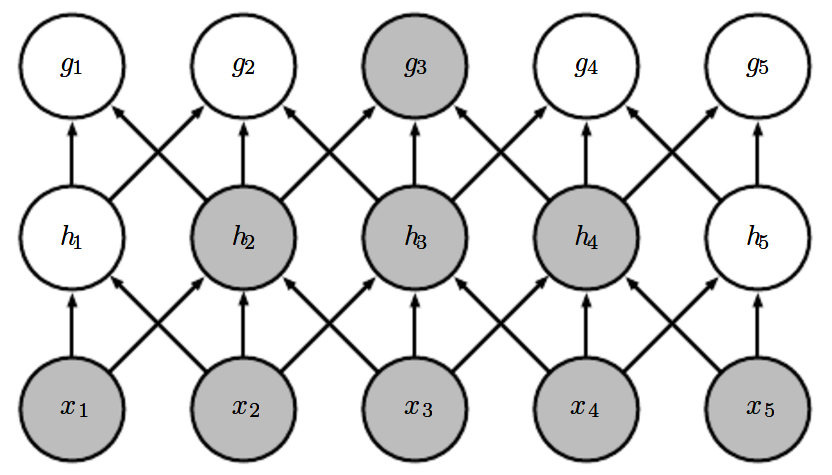
\includegraphics[width=0.7\linewidth]{images/fig94.png}
				\caption{}
				\label{fig:fig94}
				\end{figure}}
			
		\end{column}
		
		\begin{column}{0.5\textwidth}
			\begin{itemize}
				\justifying
				\setlength\itemsep{1em}
				\item<1-> But is sparse connectivity really good thing ?
				\item<2-> Aren't we losing information  (by losing interactions between some input pixels) 
				\item<3-> Well, not really
				\item<4-> The two highlighted neurons ($x_1$ \& $x_5$)$^*$\footnotetext{$^*$ Goodfellow-et-al-2016}  do not interact in $layer\ 1$
				\item<5-> But they indirectly contribute to the computation of $g_{3}$ and hence interact indirectly
			\end{itemize}
		\end{column}
		
	\end{columns}
\end{frame}

%%%%%%%%%%%%%%%%%%%%%%%%%%%%%%%%%%%%%%%%%%%%%%%%%%%%%%%%%%%%%%%%%%%%%%%%%%%%%%%%%%%%%%%%%

\begin{frame}
	\begin{columns}
		\begin{column}{0.6\textwidth}
			\begin{tikzpicture}[square/.style={regular polygon,regular polygon sides=4}]
	\onslide<3->{
		\onslide<3->{   \foreach \i in {1,...,16}
			{
                   
				\pgfmathtruncatemacro{\label}{\i};
				\node[square,draw=red!50,fill=orange!10,thick,minimum size=.2mm] (\label) at (-1*\i*0.5+1.2,-3) {};
			}
			%\end{axis}
              
			\draw [
				thick,
				decoration={
					brace,
					raise=0.5cm
				},
				decorate
			] (1) -- (16) 
			node [pos=0.5,anchor=south,yshift=-1.1cm] {16}; }
		%\end{tikzpicture}
         
		%\begin{tikzpicture}[square/.style={regular polygon,regular polygon sides=4}]
		%% Grid 4
		\onslide<3->{\draw[step=0.5cm,gray,very thin] (-4,-7) grid (-2,-5);
			\node[](img) at (-4+1,-7-0.4) {4x4 Image};
		}
         
         
		%% first row
		\onslide<3->{   \node[circle,fill=orange,inner sep=0pt,minimum size=5.5pt](A) at (-3.75,-5.25   ) {};
			\node[circle,fill=orange,inner sep=0pt,minimum size=5.5pt](B) at (-3.75+0.5,-5.25   ) {};
              
              
			%% second row
			\node[circle,fill=orange,inner sep=0pt,minimum size=5.5pt](F) at (-3.75+0.5,-5.25-0.5   ) {};
			\node[circle,fill=orange,inner sep=0pt,minimum size=5.5pt](E) at (-3.75,-5.25-0.5   ) {};
		}
         
		\onslide<3->{   
			%% 3rd row
			\node[circle,fill=magenta,inner sep=0pt,minimum size=5.5pt](K) at (-3.75+2*0.5,-5.25-2*0.5  ) {};
			\node[circle,fill=magenta,inner sep=0pt,minimum size=5.5pt](L) at (-3.75+3*0.5,-5.25-2*0.5  ) {};
              
			%% 4th row
              
			\node[circle,fill=magenta,inner sep=0pt,minimum size=5.5pt](O) at (-3.75+3*0.5,-5.25-3*0.5  ) {};
			\node[circle,fill=magenta,inner sep=0pt,minimum size=5.5pt](P) at (-3.75+2*0.5,-5.25-3*0.5  ) {};
		}
		\onslide<3->{   \node[circle,fill=orange,inner sep=0pt,minimum size=5.5pt](O) at (-6.75,-5.25-0.3   ) {};
			\node[](O) at (-6.75+1,-5.25-0.3    ) {\small{Kernel 1}};}
         
		\onslide<3->{   \node[circle,fill=magenta,inner sep=0pt,minimum size=5.5pt](O) at (-6.75,-5.25-1.5  ) {};
			\node[](O) at (-6.75+1,-5.25-1.5    ) {\small{Kernel 2}};}
         
         
		\onslide<3->{   \node[square,draw=blue!50,fill=blue!10,thick,minimum size=1mm] (11a) at (-5.5,-1.5) {};
              
			\foreach \i in {16,15,12,11}
			{
				\draw [-,thick,draw=orange] (\i) -- (11a);
			}
		}
		\onslide<3->{   \node[square,draw=blue!50,fill=blue!10,thick,minimum size=1mm] (12a) at (-0.5,-1.5) {};
              
			\foreach \i in {1,2,5,6}
			{
				\draw [-,thick,draw=magenta] (\i) -- (12a);
			}
		}
	}
    
    
\end{tikzpicture}
		\end{column}
		\begin{column}{0.4\textwidth}
			\begin{itemize}
				\justifying
				\setlength\itemsep{1em}
				\item<1-> Another characteristic of CNNs is \textbf{weight sharing}
				\item<2-> Consider the following network
				\item<4-> Do we want the kernel weights to be different for different portions of the image?
				\item<5-> Imagine that we are trying to learn a kernel that detects edges
				\item<6-> Shouldn't we be applying the same kernel at all the portions of the image?
				                
			\end{itemize}
		\end{column}
	\end{columns}
\end{frame}

%%%%%%%%%%%%%%%%%%%%%%%%%%%%%%%%%%%%%%%%%%%%%%%%%%%%%%%%%%%%%%%%%%%%%%%%%%%%%%%%%%%%%%%%%

\begin{frame}
	\begin{columns}
		\begin{column}{0.5\textwidth}
			\begin{tikzpicture}[square/.style={regular polygon,regular polygon sides=4}]
	\onslide<1->{   \foreach \i in {1,...,16}
		{
              
			\pgfmathtruncatemacro{\label}{\i};
			\node[square,draw=red!50,fill=orange!10,thick,minimum size=.2mm] (\label) at (-1*\i*0.5+1.2,-3) {};
		}
		%\end{axis}
         
		\draw [
			thick,
			decoration={
				brace,
				raise=0.5cm
			},
			decorate
		] (1) -- (16) 
		node [pos=0.5,anchor=south,yshift=-1.1cm] {16}; 
         
         
		\node[square,draw=blue!50,fill=blue!10,thick,minimum size=1mm] (11a) at (-5.5,-1.5) {};
         
		\foreach \i in {16,15,12,11}
		{
			\draw [-,thick,draw=orange] (\i) -- (11a);
		}
         
		\node[square,draw=blue!50,fill=blue!10,thick,minimum size=1mm] (12a) at (-0.5,-1.5) {};
		\foreach \i in {1,2,5,6}
		{
			\draw [-,thick,draw=magenta] (\i) -- (12a);
		}   
         
	}
	\onslide<3->
	{
         
		\foreach \i in {1,2,5,6}
		{
			\draw [-,thick,draw=orange] (\i) -- (12a);
		}
	}
    
	\onslide<7->
	{   
		\node[square,draw=blue!50,fill=blue!10,thick,minimum size=1mm] (11ab) at (-5.5+1,-1.5+0.5) {};
         
		\node[square,draw=blue!50,fill=blue!10,thick,minimum size=1mm] (12ab) at (-0.5+1,-1.5+0.5) {};
         
         
         
		\foreach \i in {16,15,12,11}
		{
			\draw [-,thick,draw=green,dashed] (\i) -- (11ab);
		}
		\foreach \i in {1,2,5,6}
		{
			\draw [-,thick,draw=green,dashed] (\i) -- (12ab);
		}
         
         
         
         
	}
    
	\onslide<8->{
         
		\node[square,draw=blue!50,fill=blue!10,thick,minimum size=1mm] (abc11) at (-5.5-1,-1.5+0.5) {};
         
		\node[square,draw=blue!50,fill=blue!10,thick,minimum size=1mm] (abc12) at (-0.5-1,-1.5+0.5) {};
         
		\foreach \i in {16,15,12,11}
		{
			\draw [-,thick,draw=magenta,dashed] (\i) -- (abc11);
		}
		\foreach \i in {1,2,5,6}
		{
			\draw [-,thick,draw=magenta,dashed] (\i) -- (abc12);
		}
	}
	%%%%%%%%%%%%5
    
\end{tikzpicture}
		\end{column}
		\begin{column}{0.5\textwidth}
			\begin{itemize}
				\justifying
				\setlength\itemsep{1em}
				\item<1-> In other words shouldn't the $orange$ and $pink$ kernels be the same 
				\item<2-> Yes, indeed
				\item<4-> This would make the job of learning easier(instead of trying to learn the same weights/kernels at different locations again and again)
				\item<5-> But does that mean we can have only one kernel?
				\item<6-> No, we can have many such kernels but the kernels will be shared by all locations in the image
				\item<9-> This is called ``weight sharing''
			\end{itemize}
		\end{column}
	\end{columns}
\end{frame}

%\begin{frame}
%    \begin{columns}
%        \column{0.5\textwidth}
%        \column{0.5\textwidth}
%       \begin{overlayarea}{\textwidth}{\textheight}
%           \begin{itemize}
%               \justifying
%               \setlength\itemsep{4em}
%               \onslide<1->{\item Because of "sparse connectivity" and "parameter sharing", CNNs exhibit translation equivariance.}
%               \onslide<2->{\item Even if the image is shifted right or left, the patterns will still be detected.}
%           \end{itemize}
%       \end{overlayarea}
%   \end{columns}
%\end{frame}

%%%%%%%%%%%%%%%%%%%%%%%%%%%%%%%%%%%%%%%%%%%%%%%%%%%%%%%%%%%%%%%%%%%%%%%%%%%%%%%%%%%%%%%%%

\begin{frame}
	\centering
	\begin{overlayarea}{\textwidth}{\textheight}
		\begin{block}{}
			\begin{itemize}
				\justifying
				\onslide<1->{\item So far, we have focused only on the convolution operation}
				\onslide<2->{\item Let us see what a full convolutional neural network looks like}
			\end{itemize}   
		\end{block}
	\end{overlayarea}
\end{frame}

%\begin{frame}
%\begin{tikzpicture}
%
%\pgfmathsetmacro{\yfactor}{0.3}
%\pgfmathsetmacro{\xfactor}{0.4}
%
%\draw [-,draw=green] (1,1) -- (1+\xfactor*0.5,1+\yfactor*0.5);
%\draw [-,draw=blue] (-1,1) -- (1+\xfactor*0.5-2,1+\yfactor*0.5);
%\draw [-,draw=blue] (1+\xfactor*0.5-2,1+\yfactor*0.5) -- (1+\xfactor*0.5,1+\yfactor*0.5);
%\draw [-,draw=blue] (1+\xfactor*0.5,1+\yfactor*0.5) -- (1+\xfactor*0.5,1+\yfactor*0.5-2);
%\draw [-,draw=blue] (1,1-2) -- (1+\xfactor*0.5,1+\yfactor*0.5-2);
%% % square
%\draw [-,draw=blue,name path = A] (-1,1) -- (1,1); % % x cahnge ->
%\draw [-,draw=blue,name path = B] (1,1) -- (1,-1); % % y change   |
%\draw [-,draw=blue,name path = C] (1,-1) -- (-1,-1); % % x change <-
%\draw [-,draw=blue,name path = D] (-1,-1) -- (-1,1); % % y change  |
%
%
%
%
%\end{tikzpicture}
%\end{frame}

%%%%%%%%%%%%%%%%%%%%%%%%%%%%%%%%%%%%%%%%%%%%%%%%%%%%%%%%%%%%%%%%%%%%%%%%%%%%%%%%%%%%%%%%%

\begin{frame}
	\vbox{
		\begin{minipage}[t][0.5\textheight][t]{\textwidth}
			\centering
			\begin{tikzpicture} 
    
    \pgfsetxvec{\pgfpoint{1cm}{0cm}}
    \pgfsetyvec{\pgfpoint{0cm}{1cm}}
    \pgfsetzvec{\pgfpoint{-0.707cm}{.707cm}}     
    
    \onslide<1->{
    
      \cuboidlabelmine{(0,-1,0)}{gray}{2}{2}{0}{32}{32}{}
      \node at (-1,-0.9,0.1) {\tiny{Input}} ;
      \begin{scope}[scale=3.5,transform shape]
        \node[] at (-0.3,-0.5,0) {A};
      \end{scope}
    }
    \onslide<1->{
      \cuboid{(2.2,-1.5,0.6)}{pink!50}{1.5}{1.5}{0}
      \cuboid{(2.2,-1.5,0.4)}{pink!50}{1.5}{1.5}{0}
      \cuboid{(2.2,-1.5,0.2)}{pink!50}{1.5}{1.5}{0}
      \cuboid{(2.2,-1.5,0)}{pink!50}{1.5}{1.5}{0}
      \cuboid{(2.2,-1.5,-0.2)}{pink!50}{1.5}{1.5}{0}
      \cuboid{(2.2,-1.5,-0.4)}{pink!50}{1.5}{1.5}{0}
      \cuboidlabelmine{(2.2,-1.5,-0.4)}{pink!50}{1.5}{1.5}{0}{28}{28}{}
      \node at (1.5,-1.3,0.6) {\tiny{Convolution Layer 1}};

      \kernel{(-0.5,-1.5,0)}{gray}{0.3}{0.3}{0}{(1.8,-2,-0.4)}

      \lenetparam{(2.2,-1.5,-0.4)}{pink!50}{1.5}{1.5}{0}{$S=1$,$F=5$,}{$K=6$,$P=0$,}{ $Param=150$}
      }
    \onslide<1->{
      \cuboid{(4.2,-2,0.6)}{blue!50}{1}{1}{0}
      \cuboid{(4.2,-2,0.4)}{blue!50}{1}{1}{0}
      \cuboid{(4.2,-2,0.2)}{blue!50}{1}{1}{0}
      \cuboid{(4.2,-2,0)}{blue!50}{1}{1}{0}
      \cuboid{(4.2,-2,-0.2)}{blue!50}{1}{1}{0}
      \cuboid{(4.2,-2,-0.4)}{blue!50}{1}{1}{0}
      \cuboidlabelmine{(4.2,-2,-0.4)}{blue!50}{1}{1}{0}{14}{14}{}
      \node at (3.5,-1.8,0.6) {\tiny{Pooling Layer 1}};

      \kernel{(1.8,-2.3,-0.4)}{gray}{0.3}{0.3}{0}{(3.8,-2.5,-0.4)}

      \lenetparam{(4.2,-2,-0.4)}{blue!50}{1}{1}{0}{$S=1$,$F=2$,}{$K=6$,$P=0$,}{ $Param=0$}
      }
    \onslide<1->{
      \cuboid{(5.9,-2,1.8)}{pink!50}{0.8}{0.8}{0}
      \cuboid{(5.9,-2,1.6)}{pink!50}{0.8}{0.8}{0}
      \cuboid{(5.9,-2,1.4)}{pink!50}{0.8}{0.8}{0}
      \cuboid{(5.9,-2,1.2)}{pink!50}{0.8}{0.8}{0}
      \cuboid{(5.9,-2,1.0)}{pink!50}{0.8}{0.8}{0}
      \cuboid{(5.9,-2,0.8)}{pink!50}{0.8}{0.8}{0}
      \cuboid{(5.9,-2,0.6)}{pink!50}{0.8}{0.8}{0}
      \cuboid{(5.9,-2,0.4)}{pink!50}{0.8}{0.8}{0}
      \cuboid{(5.9,-2,0.2)}{pink!50}{0.8}{0.8}{0}
      \cuboid{(5.9,-2,0.0)}{pink!50}{0.8}{0.8}{0}
      \cuboid{(5.9,-2,-0.2)}{pink!50}{0.8}{0.8}{0}
      \cuboid{(5.9,-2,-0.4)}{pink!50}{0.8}{0.8}{0}
      \cuboid{(5.9,-2,-0.6)}{pink!50}{0.8}{0.8}{0}
      \cuboid{(5.9,-2,-0.8)}{pink!50}{0.8}{0.8}{0}
      \cuboid{(5.9,-2,-1)}{pink!50}{0.8}{0.8}{0}
      \cuboid{(5.9,-2,-1.2)}{pink!50}{0.8}{0.8}{0}
      \cuboidlabelmine{(5.9,-2,-1.2)}{pink!50}{0.8}{0.8}{0}{10}{10}{}
      \node at (5.5,-1.8,1.8) {\tiny{Convolution Layer 2}};

     \kernel{(3.8,-2.7,-0.4)}{gray}{0.2}{0.2}{0}{(5.8,-2.8,-0.4)}

     \lenetparam{(5.9,-2,-1.2)}{pink!50}{0.8}{0.8}{0}{$S=1$,$F=5$,}{$K=16$,$P=0$,}{ $Param=2400$}
     }
    \onslide<1->{
      \cuboid{(7.9,-2.7,2.4)}{blue!50}{0.5}{0.5}{0}
      \cuboid{(7.9,-2.7,2.2)}{blue!50}{0.5}{0.5}{0}
      \cuboid{(7.9,-2.7,2)}{blue!50}{0.5}{0.5}{0}
      \cuboid{(7.9,-2.7,1.8)}{blue!50}{0.5}{0.5}{0}
      \cuboid{(7.9,-2.7,1.6)}{blue!50}{0.5}{0.5}{0}
      \cuboid{(7.9,-2.7,1.4)}{blue!50}{0.5}{0.5}{0}
      \cuboid{(7.9,-2.7,1.2)}{blue!50}{0.5}{0.5}{0}
      \cuboid{(7.9,-2.7,1)}{blue!50}{0.5}{0.5}{0}
      \cuboid{(7.9,-2.7,0.8)}{blue!50}{0.5}{0.5}{0}
      \cuboid{(7.9,-2.7,0.6)}{blue!50}{0.5}{0.5}{0}
      \cuboid{(7.9,-2.7,0.4)}{blue!50}{0.5}{0.5}{0}
      \cuboid{(7.9,-2.7,0.2)}{blue!50}{0.5}{0.5}{0}
      \cuboid{(7.9,-2.7,-0.0)}{blue!50}{0.5}{0.5}{0}
      \cuboid{(7.9,-2.7,-0.2)}{blue!50}{0.5}{0.5}{0}
      \cuboid{(7.9,-2.7,-0.4)}{blue!50}{0.5}{0.5}{0}
      \cuboid{(7.9,-2.7,-0.6)}{blue!50}{0.5}{0.5}{0}
      \cuboidlabelmine{(7.9,-2.7,-0.6)}{blue!50}{0.5}{0.5}{0}{5}{5}{}
      \node at (7.5,-2.55,2.4) {\tiny{Pooling Layer 2}};


      \kernel{(6.1,-3,-0.4)}{gray}{0.2}{0.2}{0}{(7.8,-3.2,-0.4)}

      \lenetparam{(7.9,-2.7,-0.6)}{blue!50}{0.5}{0.5}{0}{$S=1$,$F=2$,}{$K=16$,$P=0$,}{$Param=0$ }
      }
    \onslide<1->{
      \cuboid{(9.5,-3,2.2)}{magenta!50}{0.5}{0}{2.2}
      \node at (9.3,-2.85,2.2) {\tiny{FC 1(120)}};
      \draw[black] (7.9,-2.7,2.4) -- (9,-3,2.2);
      \draw[black] (7.9,-2.7,-0.6) -- (9,-3,0);
      \lenetparamnew{(9.5,-3,2.2)}{magenta!50}{0.5}{0}{2.2}{$H=120$}{$Param$}{$=48120$}

      }
    \onslide<1->{
      \cuboid{(10.5,-3,2.1)}{magenta!50}{0.5}{0}{2}
      \node at (10.3,-2.85,2.1) {\tiny{FC 2(84)}};
      \draw[black] (9.5,-3,2.2) -- (10,-3,2.1);
      \draw[black] (9.5,-3,0) -- (10,-3,0.1);
      \lenetparamnew{(10.5,-3,2.1)}{magenta!50}{0.5}{0}{2}{$H=64$}{$Param$}{$=10164$}
      }
    \onslide<1->{
      \cuboid{(11.5,-3,2.0)}{magenta!50}{0.5}{0}{1.8}
      \node at (11.3,-2.85,2.0) {\tiny{Output(10)}};
      \draw[black] (10.5,-3,2.1) -- (11,-3,2.0);
      \draw[black] (10.5,-3,0.1) -- (11,-3,0.2);
      \lenetparamnew{(11.5,-3,2.0)}{magenta!50}{0.5}{0}{1.8}{}{$Param$}{$=850$}
      }
     
    \end{tikzpicture}
			
		\end{minipage}
		\vspace{100cm}
		\begin{minipage}[t][0.5\textheight][t]{\textwidth}
			\vspace{0.4in}
			\begin{itemize}
				\justifying
				\item<2-> It has alternate convolution and pooling layers
				\item<3-> What does a pooling layer do? 
				\item<4-> Let us see
			\end{itemize}
		\end{minipage}
	}
\end{frame}

%%%%%%%%%%%%%%%%%%%%%%%%%%%%%%%%%%%%%%%%%%%%%%%%%%%%%%%%%%%%%%%%%%%%%%%%%%%%%%%%%%%%%%%%%

\begin{frame}
	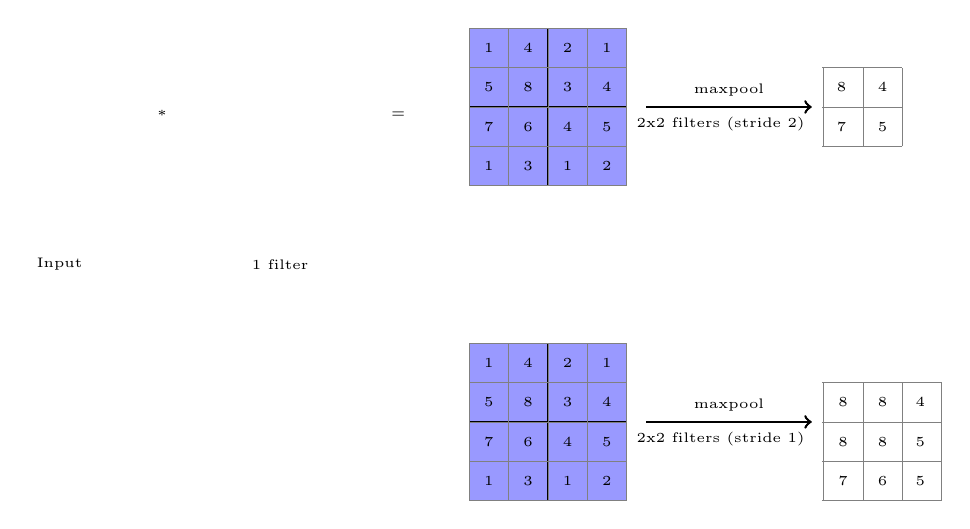
\begin{tikzpicture}
	\onslide<1->{   \renewcommand{\forefillColor}{black!50!white}
		\renewcommand{\borderColor}{white}
		\renewcommand{\toprsidefillcolor}{black!50!white!50}
		\handmadecube{0.5}{2.0}{0.7}{0}{0}
		\node(A) at (-0.2,-2.5){\tiny{Input}};}
  
	\onslide<2->{   \node(star) at (1.1,-0.6){\tiny{*}};
   
		%% filter
		\renewcommand{\forefillColor}{purple!50!white}
		\renewcommand{\borderColor}{white}
		\renewcommand{\toprsidefillcolor}{purple!50!white!50}
		\handmadecube{1.7}{2.3}{0.04}{3.5}{0.5}
		\node(A) at (2.6,-2.5){\tiny{1 filter}};
	}
  
	%%
	\onslide<3->{\node(star) at (4.1,-0.6){\tiny{=}};}
	%%
	\onslide<7>{    \filldraw[fill=blue!40!white, draw=black] (4.99999,-1.5+2) rectangle (4.99999+1,-1.5+2-1);}
  
	\onslide<8>{\filldraw[fill=blue!40!white, draw=black] (4.99999+1,-1.5+2) rectangle (4.99999+1+1,-1.5+2-1);}
  
	\onslide<9>{\filldraw[fill=blue!40!white, draw=black] (4.99999,-1.5+1) rectangle (4.99999+1,-1.5);}
  
	\onslide<10>{\filldraw[fill=blue!40!white, draw=black] (4.99999+1,-1.5+1) rectangle (4.99999+1+1,-1.5);}
	\onslide<3->{   \draw[step=0.5cm,gray,very thin] (4.99999,-1.5) grid (7,0.5);}
	%%
	
  
	\onslide<4->{   \node(A) at (5.25,0.25){\tiny{1}};
	\node(A) at (5.75,0.25){\tiny{4}};
	\node(A) at (6.25,0.25){\tiny{2}};
	\node(A) at (6.75,0.25){\tiny{1}};

	\node(A) at (5.25,-0.25){\tiny{5}};
	\node(A) at (5.75,-0.25){\tiny{8}};
	\node(A) at (6.25,-0.25){\tiny{3}};
	\node(A) at (6.75,-0.25){\tiny{4}};

	\node(A) at (5.25,-0.75){\tiny{7}};
	\node(A) at (5.75,-0.75){\tiny{6}};
	\node(A) at (6.25,-0.75){\tiny{4}};
	\node(A) at (6.75,-0.75){\tiny{5}}; 

	\node(A) at (5.25,-1.25){\tiny{1}};
	\node(A) at (5.75,-1.25){\tiny{3}};
	\node(A) at (6.25,-1.25){\tiny{1}};
	\node(A) at (6.75,-1.25){\tiny{2}};}      
	%%
	\onslide<5->{\draw[->,thick] (5.75+1.5,-0.5) -- (5.75+3.6,-0.5) node [pos=0.5,above] {\text{\tiny{maxpool}}};
		\draw[->,thick]  (5.75+1.5,-0.5) -- (5.75+3.6,-0.5) node [pos=0.45,below] {\tiny{2x2 filters (stride 2)}}; }
  
  
	\onslide<6->{   \draw[step=0.5cm,gray,very thin] (9.48559,-1) grid (10.5,0);}
	%%
	\onslide<7->{   \node(A) at (9.73,-0.25){\tiny{8}};    }
	\onslide<8->{   \node(A) at (10.25,-0.25){\tiny{4}};    }
  
	\onslide<9->{   \node(A) at (9.73,-0.75){\tiny{7}};    }
	\onslide<10->{  \node(A) at (10.25,-0.75){\tiny{5}};    }
	%%
	\onslide<14>{   \filldraw[fill=blue!40!white, draw=black] (4.99999,-5.5+2) rectangle (4.99999+1,-5.5+2-1);}
  
	\onslide<15>{   \filldraw[fill=blue!40!white, draw=black] (4.99999+0.5,-5.5+2) rectangle (4.99999+1.5,-5.5+2-1);}
  
	\onslide<17>{   \filldraw[fill=blue!40!white, draw=black] (4.99999,-5.5+2-0.5) rectangle (4.99999+1,-5.5+2-1.5);}
  
	\onslide<18>{   \filldraw[fill=blue!40!white, draw=black] (4.99999+0.5,-5.5+2-0.5) rectangle (4.99999+1.5,-5.5+2-1.5);}
      
	\onslide<19>{   \filldraw[fill=blue!40!white, draw=black] (4.99999+1,-5.5+2-0.5) rectangle (4.99999+2,-5.5+2-1.5);}
  
	\onslide<16>{   \filldraw[fill=blue!40!white, draw=black] (4.99999+1,-5.5+2) rectangle (4.99999+1+1,-5.5+2-1);}
  
	\onslide<20>{   \filldraw[fill=blue!40!white, draw=black] (4.99999,-5.5+1) rectangle (4.99999+1,-5.5);}
  
	\onslide<21>{   \filldraw[fill=blue!40!white, draw=black] (4.99999+0.5,-5.5+2-1) rectangle (4.99999+1.5,-5.5);}
  
	\onslide<22>{   \filldraw[fill=blue!40!white, draw=black] (4.99999+1,-5.5+1) rectangle (4.99999+1+1,-5.5);}
  
	
	\onslide<11->{  \draw[step=0.5cm,gray,very thin] (4.99999,-5.5) grid (7,-3.5);
		%%
		\node(A) at (5.25,-3.75){\tiny{1}};
		\node(A) at (5.75,-3.75){\tiny{4}};
		\node(A) at (6.25,-3.75){\tiny{2}};
		\node(A) at (6.75,-3.75){\tiny{1}};
   
		\node(A) at (5.25,-4.25){\tiny{5}};
		\node(A) at (5.75,-4.25){\tiny{8}};
		\node(A) at (6.25,-4.25){\tiny{3}};
		\node(A) at (6.75,-4.25){\tiny{4}};
   
		\node(A) at (5.25,-4.75){\tiny{7}};
		\node(A) at (5.75,-4.75){\tiny{6}};
		\node(A) at (6.25,-4.75){\tiny{4}};
		\node(A) at (6.75,-4.75){\tiny{5}}; 
   
		\node(A) at (5.25,-5.25){\tiny{1}};
		\node(A) at (5.75,-5.25){\tiny{3}};
		\node(A) at (6.25,-5.25){\tiny{1}};
		\node(A) at (6.75,-5.25){\tiny{2}};       
		%%
	}
  
	\onslide<12->{\draw[->,thick] (5.75+1.5,-0.5-4) -- (5.75+3.6,-0.5-4) node [pos=0.5,above] {\text{\tiny{maxpool}}};
		\draw[->,thick]  (5.75+1.5,-0.5-4) -- (5.75+3.6,-0.5-4) node [pos=0.45,below] {\tiny{2x2 filters (stride 1)}};}
      
      
	\onslide<13->{  \draw[step=0.5cm,gray,very thin] (9.48,-5.5) grid (11,-4);}
	%%
	\onslide<14->{  \node(A) at (9.75,-4.25){\tiny{8}};}
	\onslide<15->{  \node(A) at (10.25,-4.25){\tiny{8}};}
	\onslide<16->{  \node(A) at (10.73,-4.25){\tiny{4}};}
  
	\onslide<17->{  \node(A) at (9.75,-4.75){\tiny{8}};}
	\onslide<18->{  \node(A) at (10.25,-4.75){\tiny{8}};}
	\onslide<19->{  \node(A) at (10.73,-4.75){\tiny{5}};}
  
	\onslide<20->{  \node(A) at (9.75,-5.25){\tiny{7}};}
	\onslide<21->{  \node(A) at (10.25,-5.25){\tiny{6}};}
	\onslide<22->{  \node(A) at (10.73,-5.25){\tiny{5}};}

\end{tikzpicture}	    
	\begin{itemize}
		\item<23-> Instead of max pooling we can also do average pooling
	\end{itemize}
\end{frame}

%%%%%%%%%%%%%%%%%%%%%%%%%%%%%%%%%%%%%%%%%%%%%%%%%%%%%%%%%%%%%%%%%%%%%%%%%%%%%%%%%%%%%%%%%

\begin{frame}
	\begin{block}{}
		We will now see some case studies where convolution neural networks have been successful
	\end{block}
\end{frame}

%%%%%%%%%%%%%%%%%%%%%%%%%%%%%%%%%%%%%%%%%%%%%%%%%%%%%%%%%%%%%%%%%%%%%%%%%%%%%%%%%%%%%%%%%

\begin{frame}
	\begin{center}
		\Large{LeNet-5 for handwritten character recognition} 
	\end{center}
	\begin{tikzpicture} 
    
    \pgfsetxvec{\pgfpoint{1cm}{0cm}}
    \pgfsetyvec{\pgfpoint{0cm}{1cm}}
    \pgfsetzvec{\pgfpoint{-0.707cm}{.707cm}}     
    
    \onslide<1->{
    
      \cuboidlabelmine{(0,-1,0)}{gray}{2}{2}{0}{32}{32}{}
      \node at (-1,-0.9,0.1) {\tiny{Input}} ;
      \begin{scope}[scale=3.5,transform shape]
        \node[] at (-0.3,-0.5,0) {A};
      \end{scope}
    }
    \onslide<2->{
      \cuboid{(2.2,-1.5,0.6)}{pink!50}{1.5}{1.5}{0}
      \cuboid{(2.2,-1.5,0.4)}{pink!50}{1.5}{1.5}{0}
      \cuboid{(2.2,-1.5,0.2)}{pink!50}{1.5}{1.5}{0}
      \cuboid{(2.2,-1.5,0)}{pink!50}{1.5}{1.5}{0}
      \cuboid{(2.2,-1.5,-0.2)}{pink!50}{1.5}{1.5}{0}
      \cuboid{(2.2,-1.5,-0.4)}{pink!50}{1.5}{1.5}{0}
      \cuboidlabelmine{(2.2,-1.5,-0.4)}{pink!50}{1.5}{1.5}{0}{28}{28}{}
      \node at (1.5,-1.3,0.6) {\tiny{Convolution Layer 1}};

      \kernel{(-0.5,-1.5,0)}{gray}{0.3}{0.3}{0}{(1.8,-2,-0.4)}
    }
    \only<2>{
      \lenetparam{(2.2,-1.5,-0.4)}{pink!50}{1.5}{1.5}{0}{$S=1$,$F=5$,}{$K=6$,$P=0$,}{ $Param=?$}
    }
    \only<3->{
      \lenetparam{(2.2,-1.5,-0.4)}{pink!50}{1.5}{1.5}{0}{$S=1$,$F=5$,}{$K=6$,$P=0$,}{ $Param=150$}
    }
    \onslide<4->{
      \cuboid{(4.2,-2,0.6)}{blue!50}{1}{1}{0}
      \cuboid{(4.2,-2,0.4)}{blue!50}{1}{1}{0}
      \cuboid{(4.2,-2,0.2)}{blue!50}{1}{1}{0}
      \cuboid{(4.2,-2,0)}{blue!50}{1}{1}{0}
      \cuboid{(4.2,-2,-0.2)}{blue!50}{1}{1}{0}
      \cuboid{(4.2,-2,-0.4)}{blue!50}{1}{1}{0}
      \cuboidlabelmine{(4.2,-2,-0.4)}{blue!50}{1}{1}{0}{14}{14}{}
      \node at (3.5,-1.8,0.6) {\tiny{Pooling Layer 1}};

      \kernel{(1.8,-2.3,-0.4)}{gray}{0.3}{0.3}{0}{(3.8,-2.5,-0.4)}
    }
    \only<4>{
      \lenetparam{(4.2,-2,-0.4)}{blue!50}{1}{1}{0}{$S=1$,$F=2$,}{$K=6$,$P=0$,}{ $Param=?$}
    }
    \only<5->{
      \lenetparam{(4.2,-2,-0.4)}{blue!50}{1}{1}{0}{$S=1$,$F=2$,}{$K=6$,$P=0$,}{ $Param=0$}
    }
    \onslide<6->{
      \cuboid{(5.9,-2,1.8)}{pink!50}{0.8}{0.8}{0}
      \cuboid{(5.9,-2,1.6)}{pink!50}{0.8}{0.8}{0}
      \cuboid{(5.9,-2,1.4)}{pink!50}{0.8}{0.8}{0}
      \cuboid{(5.9,-2,1.2)}{pink!50}{0.8}{0.8}{0}
      \cuboid{(5.9,-2,1.0)}{pink!50}{0.8}{0.8}{0}
      \cuboid{(5.9,-2,0.8)}{pink!50}{0.8}{0.8}{0}
      \cuboid{(5.9,-2,0.6)}{pink!50}{0.8}{0.8}{0}
      \cuboid{(5.9,-2,0.4)}{pink!50}{0.8}{0.8}{0}
      \cuboid{(5.9,-2,0.2)}{pink!50}{0.8}{0.8}{0}
      \cuboid{(5.9,-2,0.0)}{pink!50}{0.8}{0.8}{0}
      \cuboid{(5.9,-2,-0.2)}{pink!50}{0.8}{0.8}{0}
      \cuboid{(5.9,-2,-0.4)}{pink!50}{0.8}{0.8}{0}
      \cuboid{(5.9,-2,-0.6)}{pink!50}{0.8}{0.8}{0}
      \cuboid{(5.9,-2,-0.8)}{pink!50}{0.8}{0.8}{0}
      \cuboid{(5.9,-2,-1)}{pink!50}{0.8}{0.8}{0}
      \cuboid{(5.9,-2,-1.2)}{pink!50}{0.8}{0.8}{0}
      \cuboidlabelmine{(5.9,-2,-1.2)}{pink!50}{0.8}{0.8}{0}{10}{10}{}
      \node at (5.5,-1.8,1.8) {\tiny{Convolution Layer 2}};

     \kernel{(3.8,-2.7,-0.4)}{gray}{0.2}{0.2}{0}{(5.8,-2.8,-0.4)} 
    }
    \only<6>{
      \lenetparam{(5.9,-2,-1.2)}{pink!50}{0.8}{0.8}{0}{$S=1$,$F=5$,}{$K=16$,$P=0$,}{ $Param=?$}
    }
    \only<7->{
      \lenetparam{(5.9,-2,-1.2)}{pink!50}{0.8}{0.8}{0}{$S=1$,$F=5$,}{$K=16$,$P=0$,}{ $Param=2400$}
    }
    
    \onslide<8->{
      \cuboid{(7.9,-2.7,2.4)}{blue!50}{0.5}{0.5}{0}
      \cuboid{(7.9,-2.7,2.2)}{blue!50}{0.5}{0.5}{0}
      \cuboid{(7.9,-2.7,2)}{blue!50}{0.5}{0.5}{0}
      \cuboid{(7.9,-2.7,1.8)}{blue!50}{0.5}{0.5}{0}
      \cuboid{(7.9,-2.7,1.6)}{blue!50}{0.5}{0.5}{0}
      \cuboid{(7.9,-2.7,1.4)}{blue!50}{0.5}{0.5}{0}
      \cuboid{(7.9,-2.7,1.2)}{blue!50}{0.5}{0.5}{0}
      \cuboid{(7.9,-2.7,1)}{blue!50}{0.5}{0.5}{0}
      \cuboid{(7.9,-2.7,0.8)}{blue!50}{0.5}{0.5}{0}
      \cuboid{(7.9,-2.7,0.6)}{blue!50}{0.5}{0.5}{0}
      \cuboid{(7.9,-2.7,0.4)}{blue!50}{0.5}{0.5}{0}
      \cuboid{(7.9,-2.7,0.2)}{blue!50}{0.5}{0.5}{0}
      \cuboid{(7.9,-2.7,-0.0)}{blue!50}{0.5}{0.5}{0}
      \cuboid{(7.9,-2.7,-0.2)}{blue!50}{0.5}{0.5}{0}
      \cuboid{(7.9,-2.7,-0.4)}{blue!50}{0.5}{0.5}{0}
      \cuboid{(7.9,-2.7,-0.6)}{blue!50}{0.5}{0.5}{0}
      \cuboidlabelmine{(7.9,-2.7,-0.6)}{blue!50}{0.5}{0.5}{0}{5}{5}{}
      \node at (7.5,-2.55,2.4) {\tiny{Pooling Layer 2}};


      \kernel{(6.1,-3,-0.4)}{gray}{0.2}{0.2}{0}{(7.8,-3.2,-0.4)}
    }
    \only<8>{
      \lenetparam{(7.9,-2.7,-0.6)}{blue!50}{0.5}{0.5}{0}{$S=1$,$F=2$,}{$K=16$,$P=0$,}{$Param=?$ }
    }
    \only<9->{
      \lenetparam{(7.9,-2.7,-0.6)}{blue!50}{0.5}{0.5}{0}{$S=1$,$F=2$,}{$K=16$,$P=0$,}{$Param=0$ }
    }
    \onslide<10->{
      \cuboid{(9.5,-3,2.2)}{magenta!50}{0.5}{0}{2.2}
      \node at (9.3,-2.85,2.2) {\tiny{FC 1(120)}};
      \draw[black] (7.9,-2.7,2.4) -- (9,-3,2.2);
      \draw[black] (7.9,-2.7,-0.6) -- (9,-3,0);
    }
    \only<10>{
      \lenetparamnew{(9.5,-3,2.2)}{magenta!50}{0.5}{0}{2.2}{$H=120$,}{$Param$}{$=?$}
    }
    \only<11->{
      \lenetparamnew{(9.5,-3,2.2)}{magenta!50}{0.5}{0}{2.2}{$H=120$,}{$Param$}{$=48120$}
    }
    \onslide<12->{
      \cuboid{(10.5,-3,2.1)}{magenta!50}{0.5}{0}{2}
      \node at (10.3,-2.85,2.1) {\tiny{FC 2(84)}};
      \draw[black] (9.5,-3,2.2) -- (10,-3,2.1);
      \draw[black] (9.5,-3,0) -- (10,-3,0.1);
    }
    \only<12>{
      \lenetparamnew{(10.5,-3,2.1)}{magenta!50}{0.5}{0}{2}{$H=84$,}{$Param$}{$=?$}
    }
    \only<13->{
      \lenetparamnew{(10.5,-3,2.1)}{magenta!50}{0.5}{0}{2}{$H=84$,}{$Param$}{$=10164$}
    }
    \onslide<14->{
	  \cuboid{(11.5,-3,2.0)}{magenta!50}{0.5}{0}{1.8}
	  \node at (11.3,-2.85,2.0) {\tiny{Output(10)}};
	  \draw[black] (10.5,-3,2.1) -- (11,-3,2.0);
	  \draw[black] (10.5,-3,0.1) -- (11,-3,0.2);
	  }
     \only<14>{
       \lenetparamnew{(11.5,-3,2.0)}{magenta!50}{0.5}{0}{1.8}{}{$Param$}{$=?$}
     }
     \only<15->{
       \lenetparamnew{(11.5,-3,2.0)}{magenta!50}{0.5}{0}{1.8}{}{$Param$}{$=850$}
     }
      

        
    \end{tikzpicture}

\end{frame}

%%%%%%%%%%%%%%%%%%%%%%%%%%%%%%%%%%%%%%%%%%%%%%%%%%%%%%%%%%%%%%%%%%%%%%%%%%%%%%%%%%%%%%%%%

\begin{frame}
	\begin{itemize}
		\item How do we train a convolutional neural network ?
	\end{itemize}
\end{frame}

%%%%%%%%%%%%%%%%%%%%%%%%%%%%%%%%%%%%%%%%%%%%%%%%%%%%%%%%%%%%%%%%%%%%%%%%%%%%%%%%%%%%%%%%%

\begin{frame}
	\begin{columns}
		\column{0.5\textwidth}
		        \begin{tikzpicture}[scale=1,transform shape]
  \tikzset{
    mstyle/.style={column sep=-\pgflinewidth,row sep=-\pgflinewidth,font=\footnotesize,},
    window/.style={draw,very thick,blue},
  }
  \matrix(convmat)[matrix of nodes,ampersand replacement=\&,column sep=4\pgflinewidth,row sep=3\pgflinewidth,
    nodes={draw,rectangle, minimum width=8mm, minimum height=8mm,font=\footnotesize,anchor=south}]{
    b\& c \& d \\
    e \& f \& g \\
    h \& i \& j \\
  };
  \foreach \j/\k [count=\i] in {2/2,3/3}{
    \onslide<\k>{
    \draw[window](convmat-1-\i.north west)rectangle(convmat-2-\j.south east);
  }}
  \foreach \j/\k [count=\i] in {2/4,3/5}{
    \onslide<\k>{
    \draw[window](convmat-2-\i.north west)rectangle(convmat-3-\j.south east);
  }}
  \matrix(filterm)[draw,right of=convmat,node distance=8em,matrix of nodes,ampersand replacement=\&,column sep=4\pgflinewidth,row sep=3\pgflinewidth,
    nodes={draw,rectangle, minimum width=8mm, minimum height=8mm,font=\footnotesize,anchor=south}]{
    \textcolor{red}{w} \& \textcolor{blue}{x} \\
    \textcolor{brown}{y} \& \textcolor{green}{z} \\
  };
  
  \onslide<2>{
  \matrix(result)[below left= 2em and -10em of convmat,node distance=11em,matrix of nodes,ampersand replacement=\&,column sep=6\pgflinewidth,row sep=6\pgflinewidth,
    nodes={draw,rectangle, minimum width=10mm, minimum height=10mm,font=\footnotesize,anchor=south},nodes in empty cells]{
    \textcolor{black}{$\ell$} \& \textcolor{white}{m}  \\
    \textcolor{white}{n} \& \textcolor{white}{o}  \\  };
  \node (text3) at ($(result) + (0,1.5)$) {\footnotesize \textsf{Output}};
  }
  \onslide<3>{
  \matrix(result)[below left = 2em and -10em of convmat,node distance=11em,matrix of nodes,ampersand replacement=\&,column sep=6\pgflinewidth,row sep=6\pgflinewidth,
    nodes={draw,rectangle, minimum width=10mm, minimum height=10mm,font=\footnotesize,anchor=south},nodes in empty cells]{
       \textcolor{black}{$\ell$} \& \textcolor{black}{m}  \\
    \textcolor{white}{n} \& \textcolor{white}{o}  \\  };
  \node (text3) at ($(result) + (0,1.5)$) {\footnotesize \textsf{Output}};
  }
  \onslide<4>{
  \matrix(result)[below left = 2em and -10em of convmat,node distance=11em,matrix of nodes,ampersand replacement=\&,column sep=6\pgflinewidth,row sep=6\pgflinewidth,
    nodes={draw,rectangle, minimum width=10mm, minimum height=10mm,font=\footnotesize,anchor=south},nodes in empty cells]{
    \textcolor{black}{$\ell$} \& \textcolor{black}{m}  \\
    \textcolor{black}{n} \& \textcolor{white}{o}  \\ 
  };
  \node (text3) at ($(result) + (0,1.5)$) {\footnotesize \textsf{Output}};
  }
  \onslide<5>{
  \matrix(result)[below left= 2em and -10em of convmat,node distance=11em,matrix of nodes,ampersand replacement=\&,column sep=6\pgflinewidth,row sep=6\pgflinewidth,
    nodes={draw,rectangle, minimum width=10mm, minimum height=10mm,font=\footnotesize,anchor=south},nodes in empty cells]{
    \textcolor{black}{$\ell$} \& \textcolor{black}{m}  \\
     \textcolor{black}{n} \& \textcolor{black}{o}  \\   };
   \node (text3) at ($(result) + (0,1.5)$) {\footnotesize \textsf{Output}}; }

  
  \node (text1) at ($(convmat) + (0,1.5)$){\footnotesize \textsf{Input}};
  \node (text2) at ($(filterm) + (0,1.5)$){\footnotesize \textsf{Kernel}};
  
  %%%%%%%%%%%%%%%%%%%%%%%Draw arrows%%%%%%%%%%%%%%%%%%%%%%%%%%%%%%%%%%%%%%%%%%%%%%%%%%%%%%%%%%%%
\end{tikzpicture}
		\vspace{-0.2in}
		\begin{itemize}
			\item <7-> We can thus train a convolution neural network using backpropagation by thinking of it as a feedforward neural network with sparse connections
		\end{itemize}
		
		\column{0.5\textwidth}
		\begin{overlayarea}{\textwidth}{\textheight}
			\begin{center}
				\begin{tikzpicture}[scale=0.8,transform shape]

\tikzstyle{input_neuron}=[circle,draw=red!50,fill=red!10,thick,minimum size=3mm]
\tikzstyle{hidden_neuron}=[circle,draw=blue!50,fill=cyan!10,thick,minimum size=3mm]
\tikzstyle{output_neuron}=[circle,draw=green!50,fill=green!10,thick,minimum size=4mm]
\tikzstyle{bias_neuron}=[circle,draw=red!50,fill=red!10,thick,minimum size=2mm]
\tikzstyle{bias_hidden_neuron}=[circle,draw=blue!50,fill=cyan!10,thick,minimum size=2mm]
\tikzstyle{bias_hidden_neuron_hi}=[circle,draw=orange,fill=cyan!10,thick,minimum size=2mm]
\tikzstyle{bias_hidden_neuron_hi_old}=[circle,draw=yellow,fill=cyan!10,thick,minimum size=2mm]
\tikzstyle{input}=[circle,draw=black!50,fill=black!20,thick,minimum size=6mm]

\node [input_neuron] (B) at (-4.0,1){\tiny{b}};
\node [input_neuron] (C) at (-3,1){\tiny{c}};
\node [input_neuron] (D) at (-2,1){\tiny{d}};
\node [input_neuron] (E) at (-1,1){\tiny{e}};
\node [input_neuron] (F) at (0,1){\tiny{f}};
\node [input_neuron] (G) at (1,1){\tiny{g}};
\node [input_neuron] (H) at (2,1){\tiny{h}};
\node [input_neuron] (I) at (3,1){\tiny{i}};
\node [input_neuron] (J) at (4,1){\tiny{j}};

\node [hidden_neuron] (O) at (2,3){\tiny{o}};
\node [hidden_neuron] (N) at (1,3){\tiny{n}};
\node [hidden_neuron] (M) at (-1,3){\tiny{m}};
\node [hidden_neuron] (L) at (-2,3){\tiny{l}};

\node [output_neuron] (T) at (0,4){};
\onslide<1->{
	
	\draw [->] (B) -- (L);
	\draw [->] (C) -- (L);
	\draw [->,color=black] (D) -- (L);
	\draw [->] (E) -- (L);
	\draw [->,color=black] (F) -- (L);
	\draw [->,color=black] (G) -- (L);
	\draw [->,color=black] (H) -- (L);
	\draw [->,color=black] (I) -- (L);
	\draw [->,color=black] (J) -- (L);



	
	\draw [->] ($(B) + (0,-0.5)$) -- (B);
	\draw [->] ($(C) + (0,-0.5)$) -- (C);
	\draw [->] ($(D) + (0,-0.5)$) -- (D);
	\draw [->] ($(E) + (0,-0.5)$) -- (E);
	\draw [->] ($(F) + (0,-0.5)$) -- (F);
	\draw [->] ($(G) + (0,-0.5)$) -- (G);
	\draw [->] ($(H) + (0,-0.5)$) -- (H);
	\draw [->] ($(I) + (0,-0.5)$) -- (I);
	\draw [->] ($(J) + (0,-0.5)$) -- (J);

	\draw [->,color=black] (B) -- (M);
	\draw [->] (C) -- (M);
	\draw [->] (D) -- (M);
	\draw [->,color=black] (E) -- (M);
	\draw [->] (F) -- (M);
	\draw [->] (G) -- (M);
	\draw [->,color=black] (H) -- (M);
	\draw [->,color=black] (I) -- (M);
	\draw [->,color=black] (J) -- (M);


	\draw [->,color=black] (B) -- (N);
	\draw [->,color=black] (C) -- (N);
	\draw [->,color=black] (D) -- (N);
	\draw [->] (E) -- (N);
	\draw [->] (F) -- (N);
	\draw [->,color=black] (G) -- (N);
	\draw [->] (H) -- (N);
	\draw [->] (I) -- (N);
	\draw [->,color=black] (J) -- (N);


	\draw [->,color=black] (B) -- (O);
	\draw [->,color=black] (C) -- (O);
	\draw [->,color=black] (D) -- (O);
	\draw [->,color=black] (E) -- (O);
	\draw [->] (F) -- (O);
	\draw [->] (G) -- (O);
	\draw [->,color=black] (H) -- (O);
	\draw [->] (I) -- (O);
	\draw [->] (J) -- (O);

	\draw [->] (L) -- (T);
	\draw [->] (M) -- (T);
	\draw [->] (N) -- (T);
	\draw [->] (O) -- (T);

}
\onslide<2->{
	
	\draw [->,color=red, line width=1.5] (B) -- (L);
	\draw [->,color=blue, line width=1.5] (C) -- (L);
	\draw [->,color=black!10] (D) -- (L);
	\draw [->,color=brown, line width=1.5] (E) -- (L);
	\draw [->,color=green, line width=1.5] (F) -- (L);
	\draw [->,color=black!10] (G) -- (L);
	\draw [->,color=black!10] (H) -- (L);
	\draw [->,color=black!10] (I) -- (L);
	\draw [->,color=black!10] (J) -- (L);


}

\onslide<3->{
	
	\draw [->,color=red, line width=1.5] (C) -- (M);
	\draw [->,color=blue, line width=1.5] (D) -- (M);
	\draw [->,color=black!10] (B) -- (M);
	\draw [->,color=brown, line width=1.5] (F) -- (M);
	\draw [->,color=green, line width=1.5] (G) -- (M);
	\draw [->,color=black!10] (E) -- (M);
	\draw [->,color=black!10] (H) -- (M);
	\draw [->,color=black!10] (I) -- (M);
	\draw [->,color=black!10] (J) -- (M);


}

\onslide<4->{
	
	\draw [->,color=red, line width=1.5] (E) -- (N);
	\draw [->,color=blue, line width=1.5] (F) -- (N);
	\draw [->,color=black!10] (B) -- (N);
	\draw [->,color=brown, line width=1.5] (H) -- (N);
	\draw [->,color=green, line width=1.5] (I) -- (N);
	\draw [->,color=black!10] (C) -- (N);
	\draw [->,color=black!10] (D) -- (N);
	\draw [->,color=black!10] (I) -- (N);
	\draw [->,color=black!10] (G) -- (N);


}

\onslide<5->{
	
	\draw [->,color=red, line width=1.5] (F) -- (O);
	\draw [->,color=blue, line width=1.5] (I) -- (O);
	\draw [->,color=black!10] (B) -- (O);
	\draw [->,color=brown, line width=1.5] (G) -- (O);
	\draw [->,color=green, line width=1.5] (J) -- (O);
	\draw [->,color=black!10] (C) -- (O);
	\draw [->,color=black!10] (D) -- (O);
	\draw [->,color=black!10] (E) -- (O);
	\draw [->,color=black!10] (H) -- (O);


}
\end{tikzpicture}
			\end{center}
			\begin{center}
				%\begin{block}{}
				\begin{itemize}
					\item <1-> A CNN can be implemented as a feedforward neural network
					\item <2-> wherein only a few weights(in color) are active
					\item <3-> the rest of the weights (in gray) are zero
					      %\item <8-> we can thus train a convolution neural network using backpropagation by thinking of it as a feedforward neural network with sparse connections
				\end{itemize}
				%\end{block}
			\end{center}
		\end{overlayarea}
	\end{columns}
\end{frame}



